\documentclass[letterpaper, oneside, 11pt]{book}
\usepackage[left=1in, right=1in, top=0.75in]{geometry}
\usepackage[svgnames]{xcolor}
\usepackage{graphicx}
\usepackage{appendix}
\usepackage{float}
\usepackage{setspace}
\usepackage[sfdefault]{roboto}
\usepackage{xcolor}
\usepackage{sectsty}
\usepackage[colorlinks=true, linkcolor=gray]{hyperref}
\usepackage[utf8]{inputenc}
\usepackage{hyperref}
\usepackage{tabularx}
\usepackage{longtable}
\usepackage{listings}
\usepackage{glossaries-extra}

\setabbreviationstyle[acronym]{long-short}
\loadglsentries{../Common/defn}
\makenoidxglossaries

\definecolor{MyBlue}{rgb}{0.03, 0.27, 0.49}
\chapterfont{\color{MyBlue}}
\sectionfont{\color{MyBlue}}
\subsectionfont{\color{MyBlue}}
\setlength{\parindent}{0pt}

\begin{document}
%%========================================================================
\begin{titlepage}
	\raggedleft
	\begin{figure}[H]
	\centering
		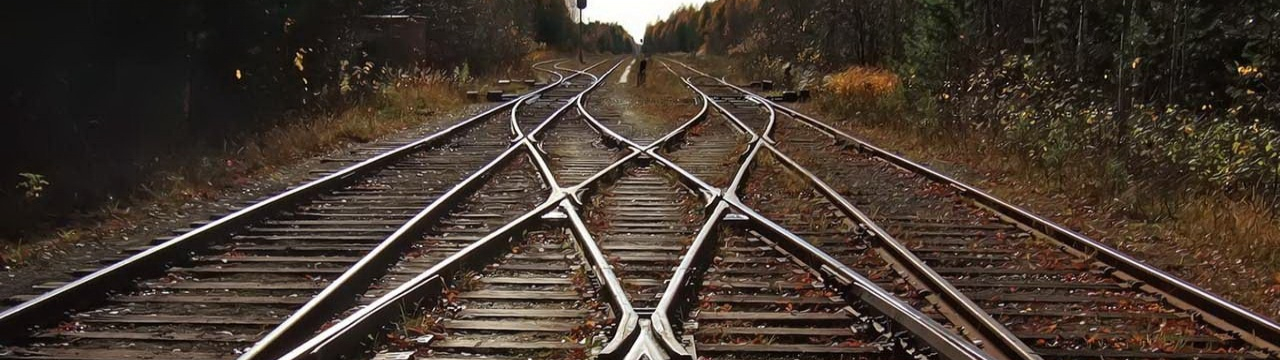
\includegraphics[scale=1.53]{../Images/railway_track.jpg}
	\label{fig:track}
\end{figure}
	\vspace*{0.167\textheight}
	\textbf{\LARGE MRIM Installation and Operations Manual}\\[\baselineskip]
    \textbf{\textcolor{MyBlue}{\Huge R\Large ailway \Huge A\Large dministration and \Huge I\Large nformation \Huge L\Large ogical \Huge S\Large ystem}}\\[\baselineskip]
	{\Large \textit{RAILS for Model Railroads}}
	\vfill
    \vspace*{\baselineskip}
	{\small David Bristow}

	{\small Version 1.0.1}
	
	{\small \today}
	\vspace*{3\baselineskip}
\end{titlepage}
%%========================================================================
\tableofcontents
%% copyright notice
%%========================================================================
\chapter{Model Railroad Information Manager}
\section{Introduction}
\gls{rails} is a software model and implementation of an automated system to assist the model railroader achieve realism in the operation of a model railroad.
The \gls{rails} system design describes the system's architecture, components, and interfaces and can be found at \href{https://github.com/djbristow/RAILS/blob/master/Documentation/rails-system.pdf}{RAILS System Design and implementation}.
There are four user interface \glspl{spa} that provide different aspects of \gls{rails} they are:
\begin{itemize}
  \item \gls{rsrm} provides a user with a web application to show, when an RFID tag is read, the road name and number of the rolling stock associated with that tag.
  \item \gls{mrim} the focus of this manual, allows the user to create, update and delete model railroad assets, such as:
    \begin{itemize}
		\item manage lists of items found in model railroads:
        \begin{itemize}
 		    \item Rolling Stock
 		    \item DCC decoders
 		    \item AAR Codes
 		    \item Images
 		    \item Companies
 		    \item Structures
	    \end{itemize}
		\item creates PDF reports; and
        \begin{itemize}
 		    \item AAR Codes
 		    \item Companies
 		    \item Images
 		    \item RFID
 		    \item Rolling Stock sortable by Road Name and Road Number or AAR Code or Status
	    \end{itemize}
		\item exports and imports inventories in CSV files.
	\end{itemize}
  \item \gls{mppm} allows the user to enter information about their projects and purchases; and
  \item \gls{mrlm} allows the user to enter information about their layout and control elements of it.
\end{itemize}
\section{Components}
The implementation of \gls{mrim} consists of the following microservices components:
\begin{itemize}
    \item \gls{mrfm} provides the user the ability to upload image files;
    \item images is a repository for the images of rollingstock and structures;
    \item \gls{rids} provides \gls{rest} access to railroad inventory collections including \gls{rs};
    \item MongoDB a NoSQL database program that stores data records as documents which are gathered in collections. A database stores one or more collections of documents;
    \item \gls{mr} Data is the document repository, used by MongoDB, to store complete collections of items such as \gls{rs}, industries (producers and consumers), track elements, 
turnouts, projects, purchases, etc. in support of \gls{rails}; and
    \item \gls{mrim} is the \gls{spa}.
\end{itemize}
\begin{figure}[H]
	\centering
		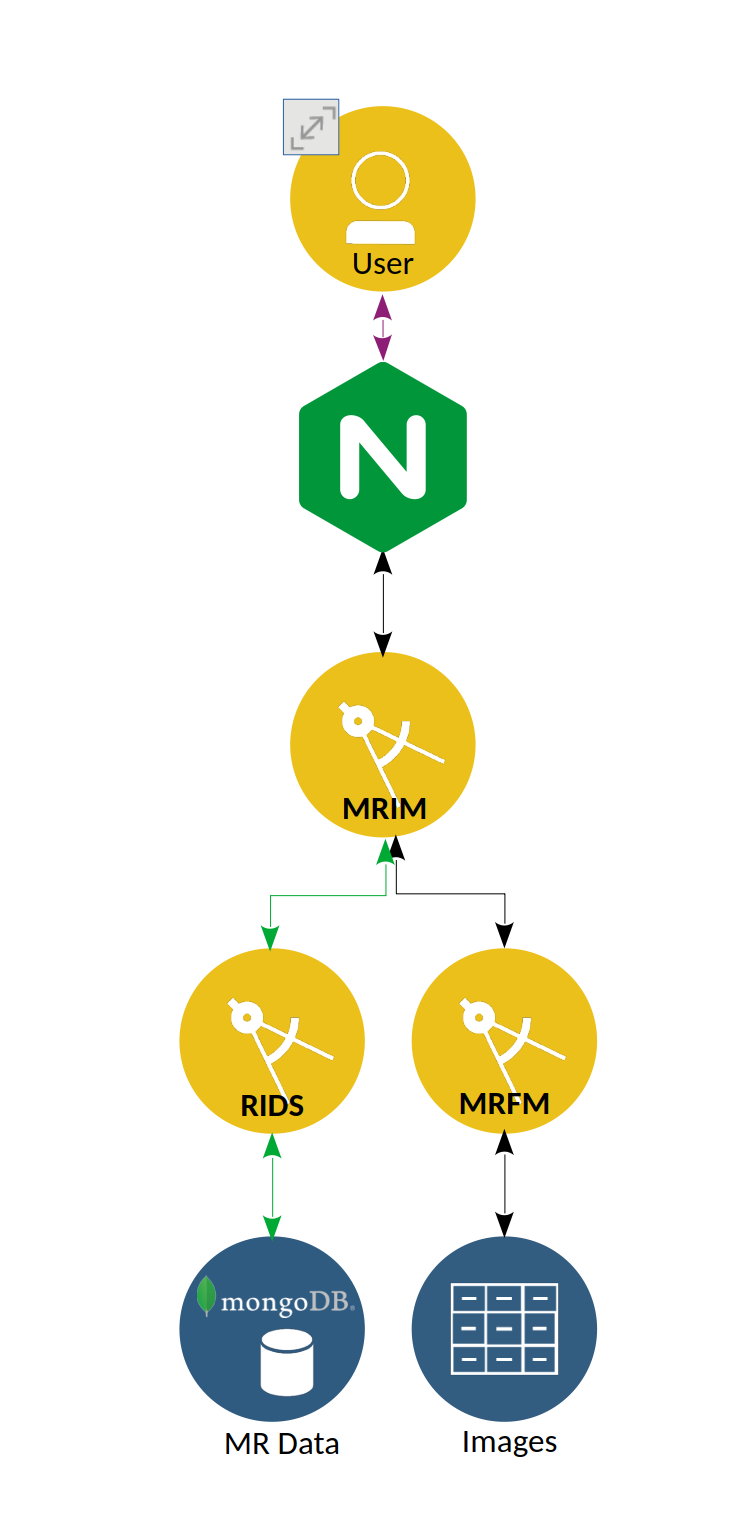
\includegraphics[scale=0.2]{./images/mrim-design.png}
	\caption{Microservices Components}
	\label{fig:rsms-ms-components}
\end{figure}
\section{System Components}
Three system components that make up this subsystem:
\begin{itemize}
    \item Network is a \gls{tcpip} communication medium that connects the client (one or more) to the host running the \gls{mrim} docker containers;
    \item Server is a computer that runs \gls{mrim} microservices components; and
    \item Client\footnote{A web browser may be used on the Server and client machine is omitted} is a computer that runs a web browser to display the \gls{mrim} \gls{spa}.
\end{itemize}

\begin{figure}[H]
	\centering
		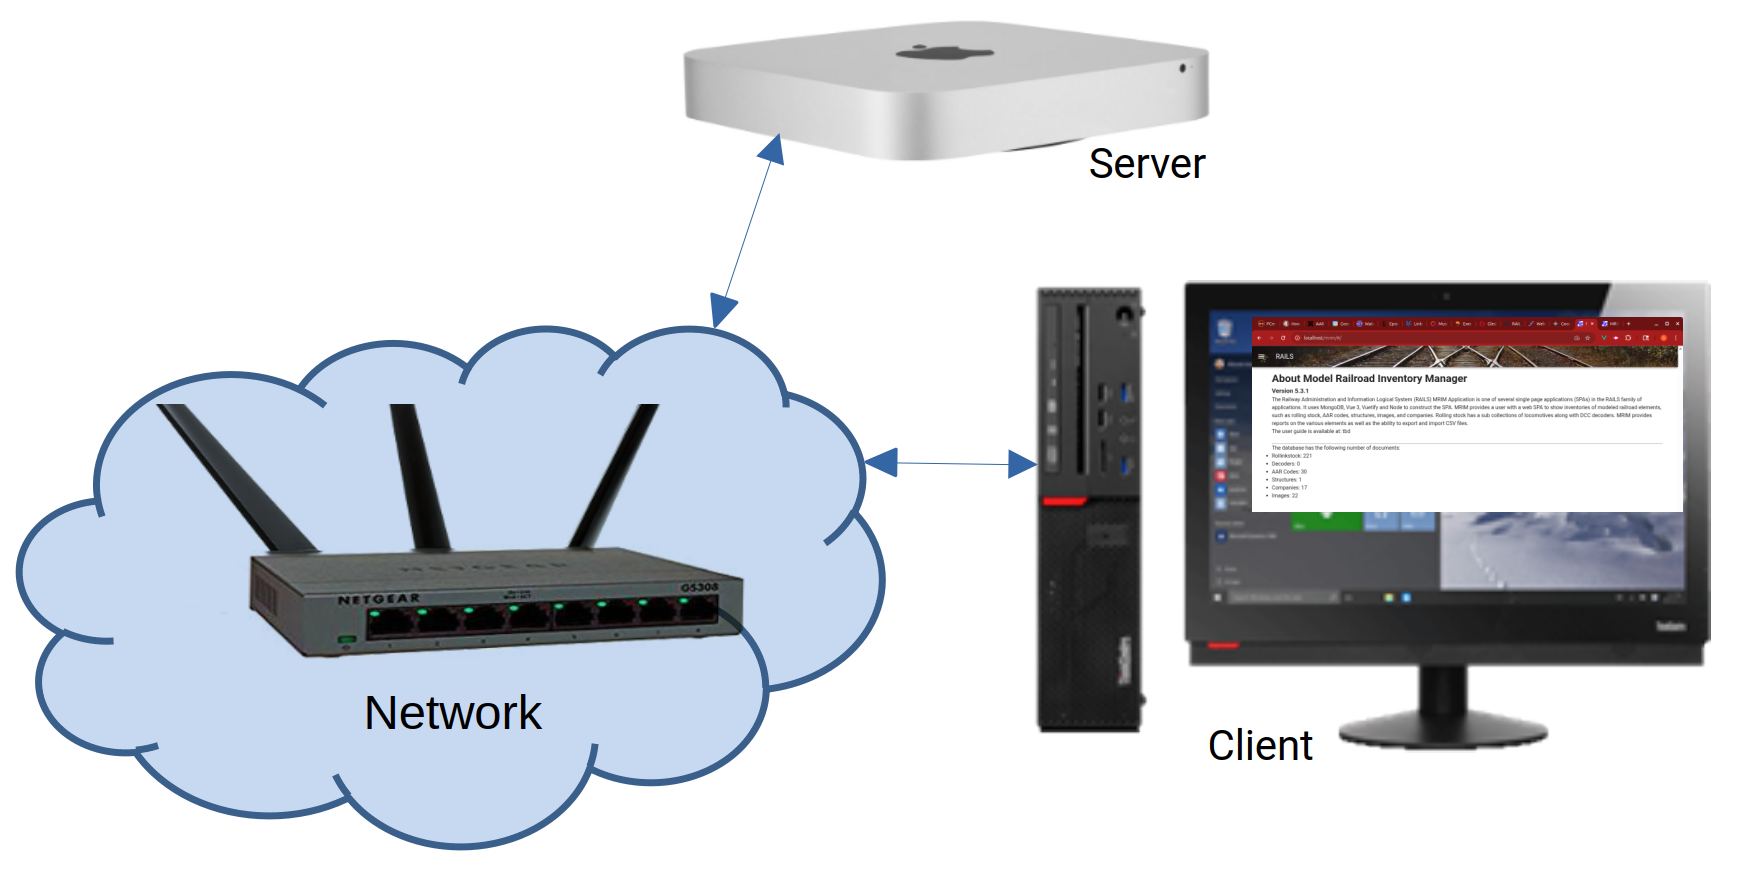
\includegraphics[scale=0.25]{./images/mrim-system.png}
	\caption{System Components}
	\label{fig:mrim-system-components}
\end{figure}

\chapter{Docker Set Up}
\label{ch:installandrun}
\section{Docker Installation}
\label{sec:dockerinstall}
The \gls{rails} \glspl{spa} are implemented as Docker containers. The Docker containers are built and pushed to Docker Hub. The Docker containers are then pulled from Docker Hub and run on the host machine. 
The host machine must have Docker installed. Docker is a platform for developing, shipping, and running applications in containers. Docker can be installed on Windows, macOS, and Linux. 
The installation instructions for Docker can be found at \href{https://docs.docker.com/get-docker/}{https://docs.docker.com/get-docker/}.
\section{Docker Compose Installation}
\label{sec:dockercomposeinstall}
Docker Compose is a tool for defining and running multi-container Docker applications. Docker Compose uses a \gls{yaml} file to configure the application's services. The installation instructions\footnote{Note that for Microsoft Windows the installation of the \gls{gui} Docker Desktop automatically installs Docker Compose.} for Docker Compose can be found at \href{https://docs.docker.com/compose/install/}{https://docs.docker.com/compose/install/}.
\section{Broker Configuration}
\label{sec:brokerconfig}
The \gls{rails} \glspl{spa} use the Mosquitto broker to communicate with each other. The Mosquitto broker is an open-source message broker that implements the \gls{mqtt} protocol. The Mosquitto broker must be configured to allow the \gls{rails} \glspl{spa} to communicate with each other. The Mosquitto broker configuration file must be edited to allow the \gls{rails} \glspl{spa} to communicate with each other. The configuration file is found in the virtual storage whose volume name is “mosquitto”. To establish and modify the configuration file the following steps are taken:
\begin{enumerate}
    \item Create a folder/directory ``RAILS'' and open a terminal from that folder/directory (all docker commands should be run in that terminal).
    \item Create a Docker volume for the Mosquitto broker.
    \begin{verbatim}
    docker volume create --name mosquitto
    \end{verbatim}
    \item Run a Docker container for the first time the Mosquitto broker, which will create the initial configuration file.
    \begin{verbatim}
    docker run -it --name myMqttBrkr -p 1883:1883 -p 9001:9001 --rm
    -v mosquitto:/mosquitto -d eclipse-mosquitto
    \end{verbatim}
    \item Stop the broker container.
    \begin{verbatim}    
    docker stop myMqttBrkr
    \end{verbatim}
    \item Locate the configuration file in the "mosquitto" volume.
    \begin{verbatim}    
    docker inspect mosquitto
    \end{verbatim}
    \item Edit the configuration file modifying or adding the following lines:
    \begin{verbatim}
    listener 1883
    allow_anonymous true
    socket_domain ipv4
    \end{verbatim}
\end{enumerate}
\section{Create the RAILS Docker Environment}
\label{sec:railsdockerenv}
The \gls{rails} \glspl{spa} are implemented as Docker containers that require an environment to run in. To create that environment, the following steps are taken:
\begin{enumerate}
    \item Create a Docker volume for the Rails database.
    \begin{verbatim}
    docker volume create --name myRailsDb  
    \end{verbatim}
    \item Create a Docker volume for the Rails images.
    \begin{verbatim}
    docker volume create --name myRailsImages
    \end{verbatim}
    \item Create a Docker network for the Rails containers to communicate over.
    \begin{verbatim}
    docker network create myRailsNet
    \end{verbatim}
\end{enumerate}
\section{Modify the Model Railroad Name}
To change the name of the model railroad displayed in the \glspl{spa} from "KJ\&C RR" to a name of choice edit the docker-compose.yaml file.
Find the text at line \#67 for the \gls{spa} \gls{mppm}:
    \begin{verbatim}
- MRNAME=KJ&C RR
    \end{verbatim}
Edit the string "KJ\&C RR" to the name of choice. Then repeat for each of the other \glspl{spa} as follows:
\begin{itemize}
    \item at line \#104 for the \gls{spa} \gls{mrim}
    \item at line \#152 for the \gls{spa} \gls{rsrm}
    \item at line \#197 for the \gls{spa} \gls{mrlm}
\end{itemize}
\section{Run the RAILS Docker Containers}
\label{sec:railsdockercontainers}
The Docker containers are pulled from Docker Hub and run on the host machine. To run all of the \gls{rails} Docker containers retrieve the \gls{yaml} ``docker-compose.yaml'' file from the \gls{rails} GitHub repository found at \href{https://github.com/djbristow/RAILS/tree/master/Docker%20Based}{my GitHub repository}. Additionally retreive the ``nginx.conf'' file from \gls{rails} GitHub repository. Be sure that both files are put into the ``RAILS'' folder/directory. 
To fetch the Docker images, create the containers, and start the conatiners running execute the following command in the terminal opened in the ``RAILS'' folder/directory:
\begin{verbatim}
docker compose up -d
\end{verbatim}
This command will pull the Docker images from Docker Hub and run the containers in detached mode. The \gls{rails} \glspl{spa} will be running in the background, and the terminal will return to the command prompt.
The \gls{rails} \glspl{spa} will be running on the host machine.
Point a browser, on the host machine, to the following URLs to access the \gls{rails} \glspl{spa}:
\begin{itemize}
    \item \gls{mrim} \gls{spa} - \href{http://localhost/mrim}{http://localhost/mrim} (or \texttt{http://\textless MACHINE\_IP\textgreater /mrim/})
    \item \gls{rsrm} \gls{spa} - \href{http://localhost/rsrm}{http://localhost/rsrm} (or \texttt{http://\textless MACHINE\_IP\textgreater /rsrm/})
    \item \gls{mppm} \gls{spa} - \href{http://localhost/mppm}{http://localhost/mppm} (or \texttt{http://\textless MACHINE\_IP\textgreater /mppm/})
    \item \gls{mrlm} \gls{spa} - \href{http://localhost/mrlm}{http://localhost/mrlm} (or \texttt{http://\textless MACHINE\_IP\textgreater /mrlm/})
\end{itemize}
Where \textless MACHINE\_IP\textgreater\ is the IP address of the host machine running the Docker containers. The \gls{rails} \glspl{spa} can be accessed from any browser on any Personal Computer (PC) in the network.
\section{Stop and Remove the RAILS Docker Containers}
\label{sec:stopremoverailsdockercontainers}
To stop and remove the \gls{rails} Docker containers, the following command is used:
\begin{verbatim}
docker compose down
\end{verbatim}


\newcommand{\hamburger}{%
  \vbox{%
    \hrule width 1em height 1pt\smallskip
    \hrule width 1em height 1pt\smallskip
    \hrule width 1em height 1pt}%
}
\chapter{MRIM Operations}
\gls{rsrm} simplifies identifying rollingstock by associating \gls{rfid} tags with specific road names and numbers.
When a connected reader reads an \gls{rfid} tag, \gls{rsrm} searches its database for a matching entry. If a match is found, the application displays the corresponding 
road name and number of the rollingstock. If no match is found, the application provides input fields for the user to manually enter this information, 
creating a new association in the database.

\section{About Page}

The intial page when the application is opened in a web browser provides:
\begin{itemize}
    \item A version number of the application;
    \item A concise overview of the application's purpose and technology stack;
    \item The current database statistics indicating:
    \begin{itemize}
        \item The number of rollingstock entries in the database and how many have \gls{rfid} tags; and
        \item The number of micro-controllers in the database and how many are RFID readers.
    \end{itemize}
\end{itemize}
Figure \ref{fig:about1} shows the "About" page of the RAILS RS RFID Manager application.

\begin{figure}[H]
    \centering
    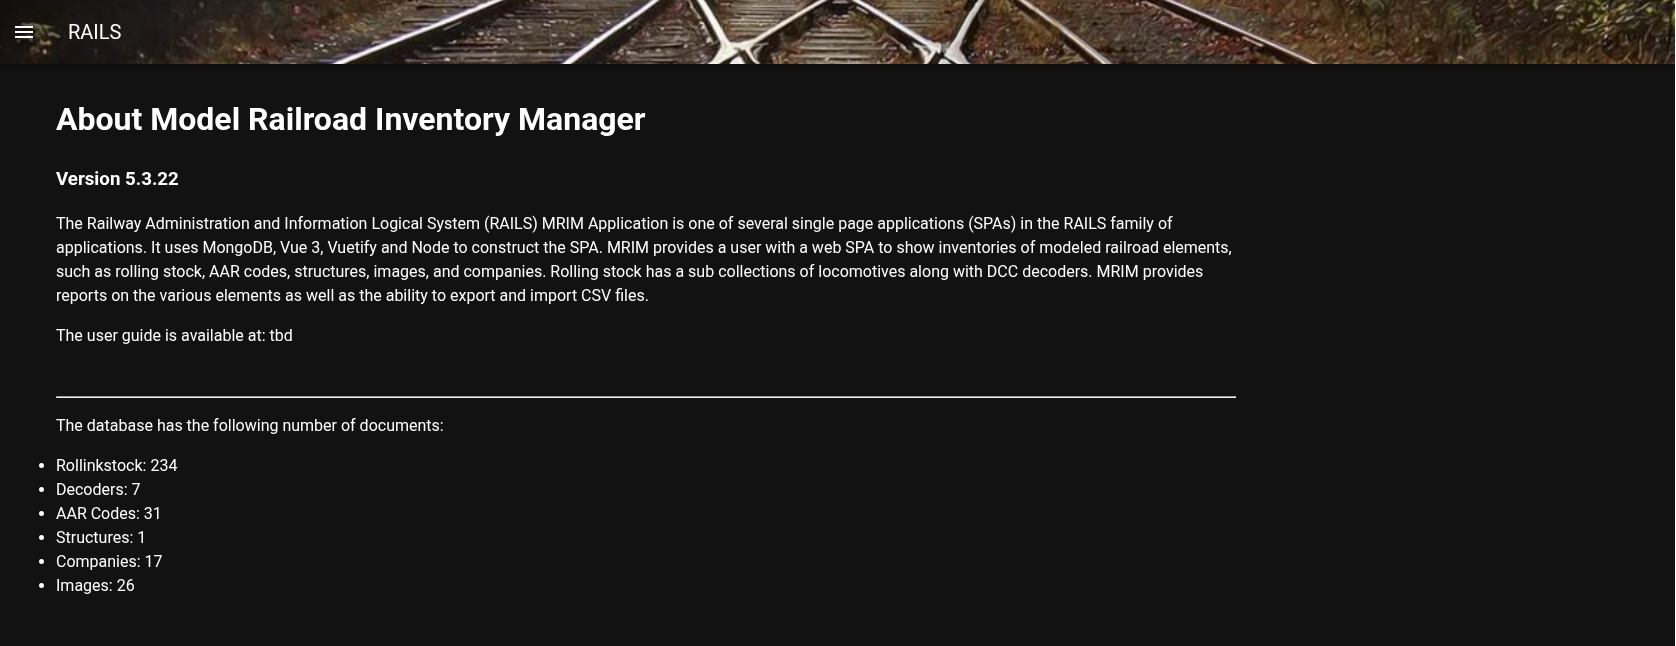
\includegraphics[scale=0.25]{./images/about.png}
    \caption{About Page}
    \label{fig:about1}
\end{figure}

The hamburger menu icon \hamburger, to the left of "RAILS" represents a hidden navigation menu that can be toggled open and closed. 
When the icon is clicked or tapped on the menu for navigation to different pages of this application is revealed. This menu  
contains the links: "Reader," "Admin," "Rollingstock," "AAR Codes," "About" (this page). 
Figure \ref{fig:about2} shows the "About" page with the navigation menu opened.

\begin{figure}[H]
    \centering
    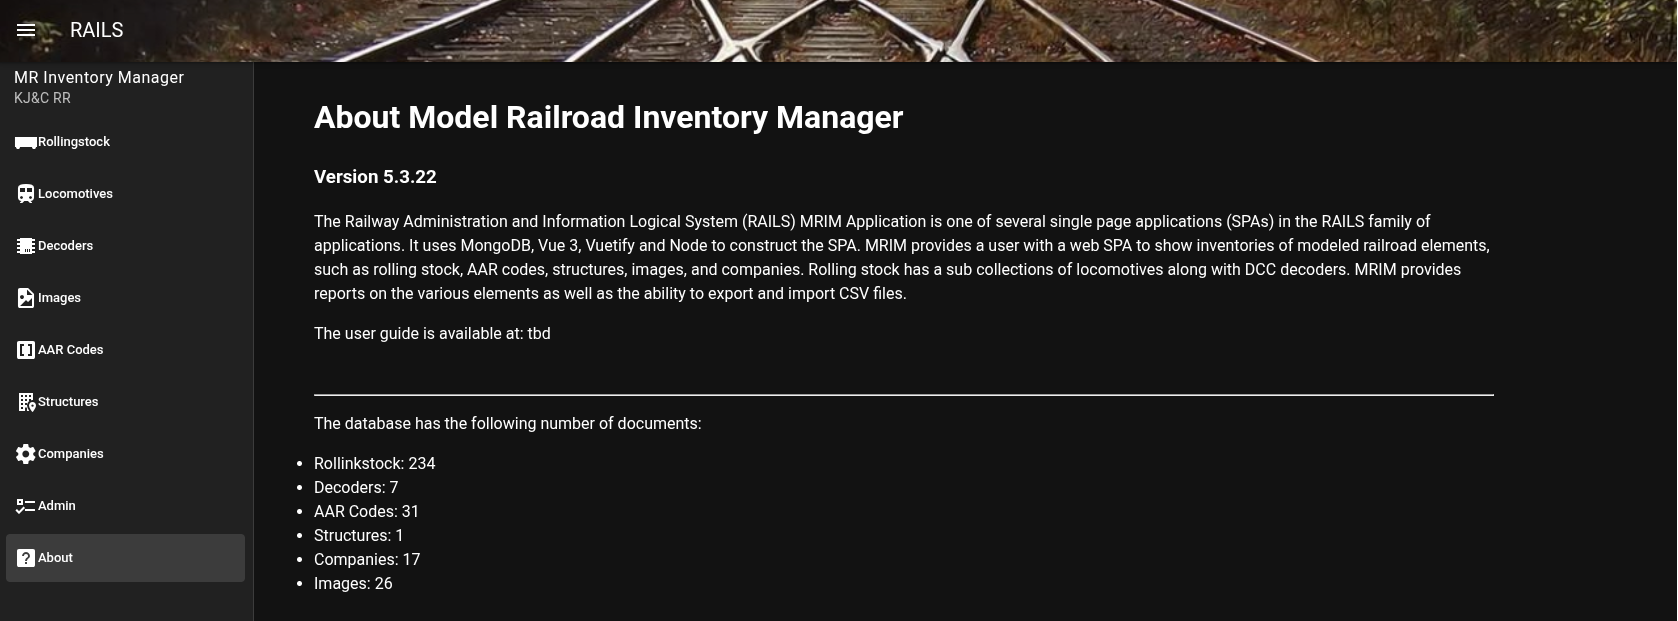
\includegraphics[scale=0.25]{./images/about-hamburger.png}
    \caption{Sidemenu}
    \label{fig:about2}
\end{figure}

\section{Rolling Stock Management}

The Rollingstock view provides a complete inventory of all rolling stock registered in the system. Selecting "Rollingstock" from the navigation drawer displays the main tabular view containing all registered pieces, including key attributes such as Road Name, Road Number, AAR Code, Description, Color, and available Action buttons. Figure \ref{fig:rollingstock} displays the main Rollingstock table page.

\begin{figure}[H]
    \centering
    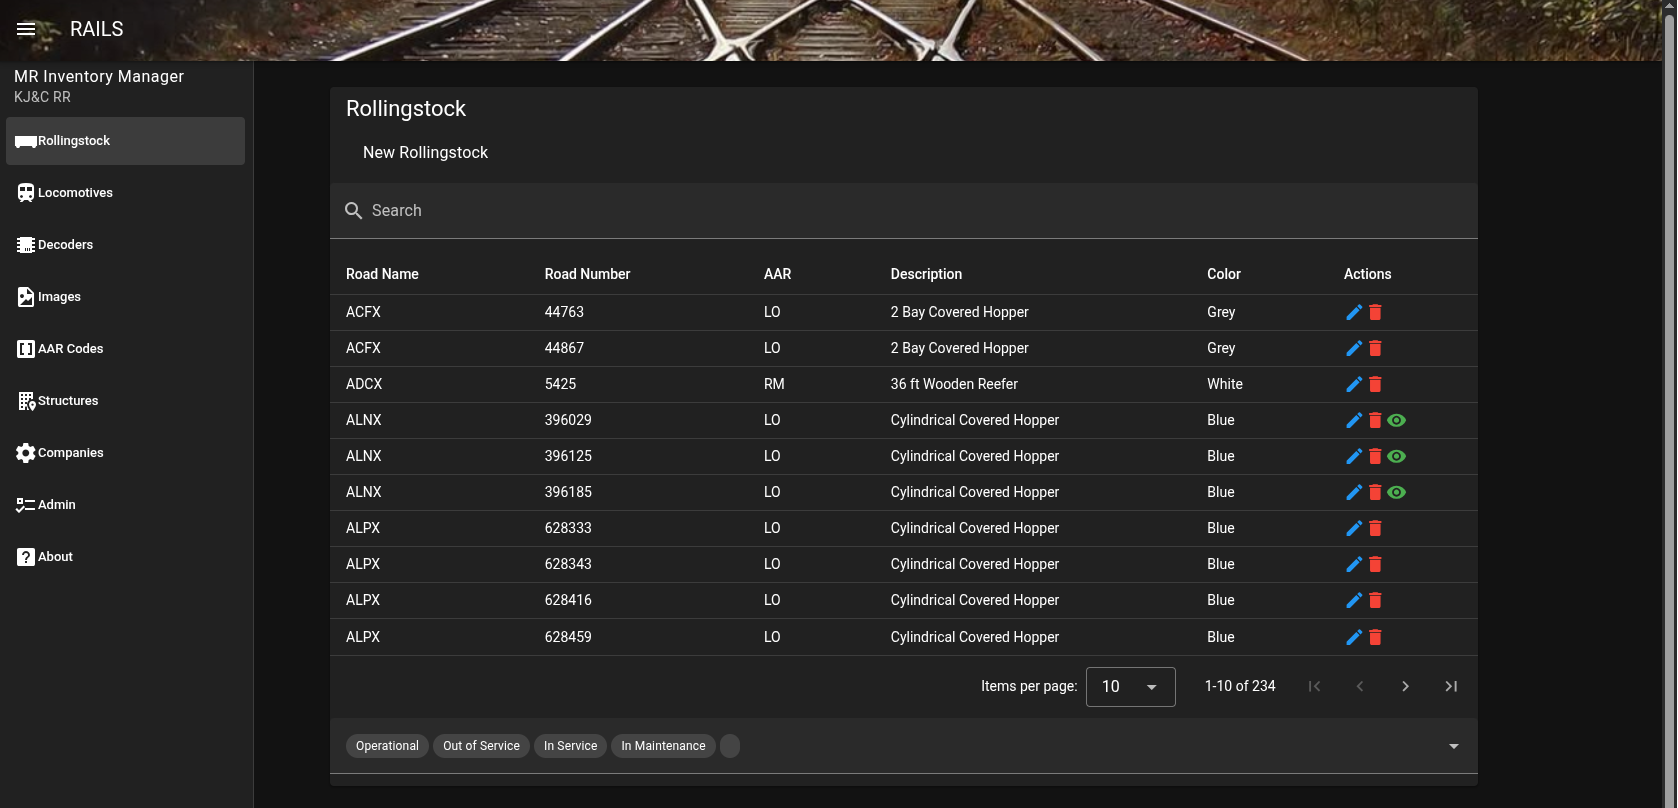
\includegraphics[width=0.85\textwidth]{./images/rollingstock.png}
    \caption{Rollingstock Page}
    \label{fig:rollingstock}
\end{figure}

\subsection{Page Quantity Selection}

The table displays items in paginated format. Users can control the number of rolling stock items shown per page using the dropdown selector located at the bottom right of the table. Available options include 10, 25, 50, 100, or All items. Figure \ref{fig:rs-pg-qty} illustrates changing the items per page display count.

\begin{figure}[H]
    \centering
    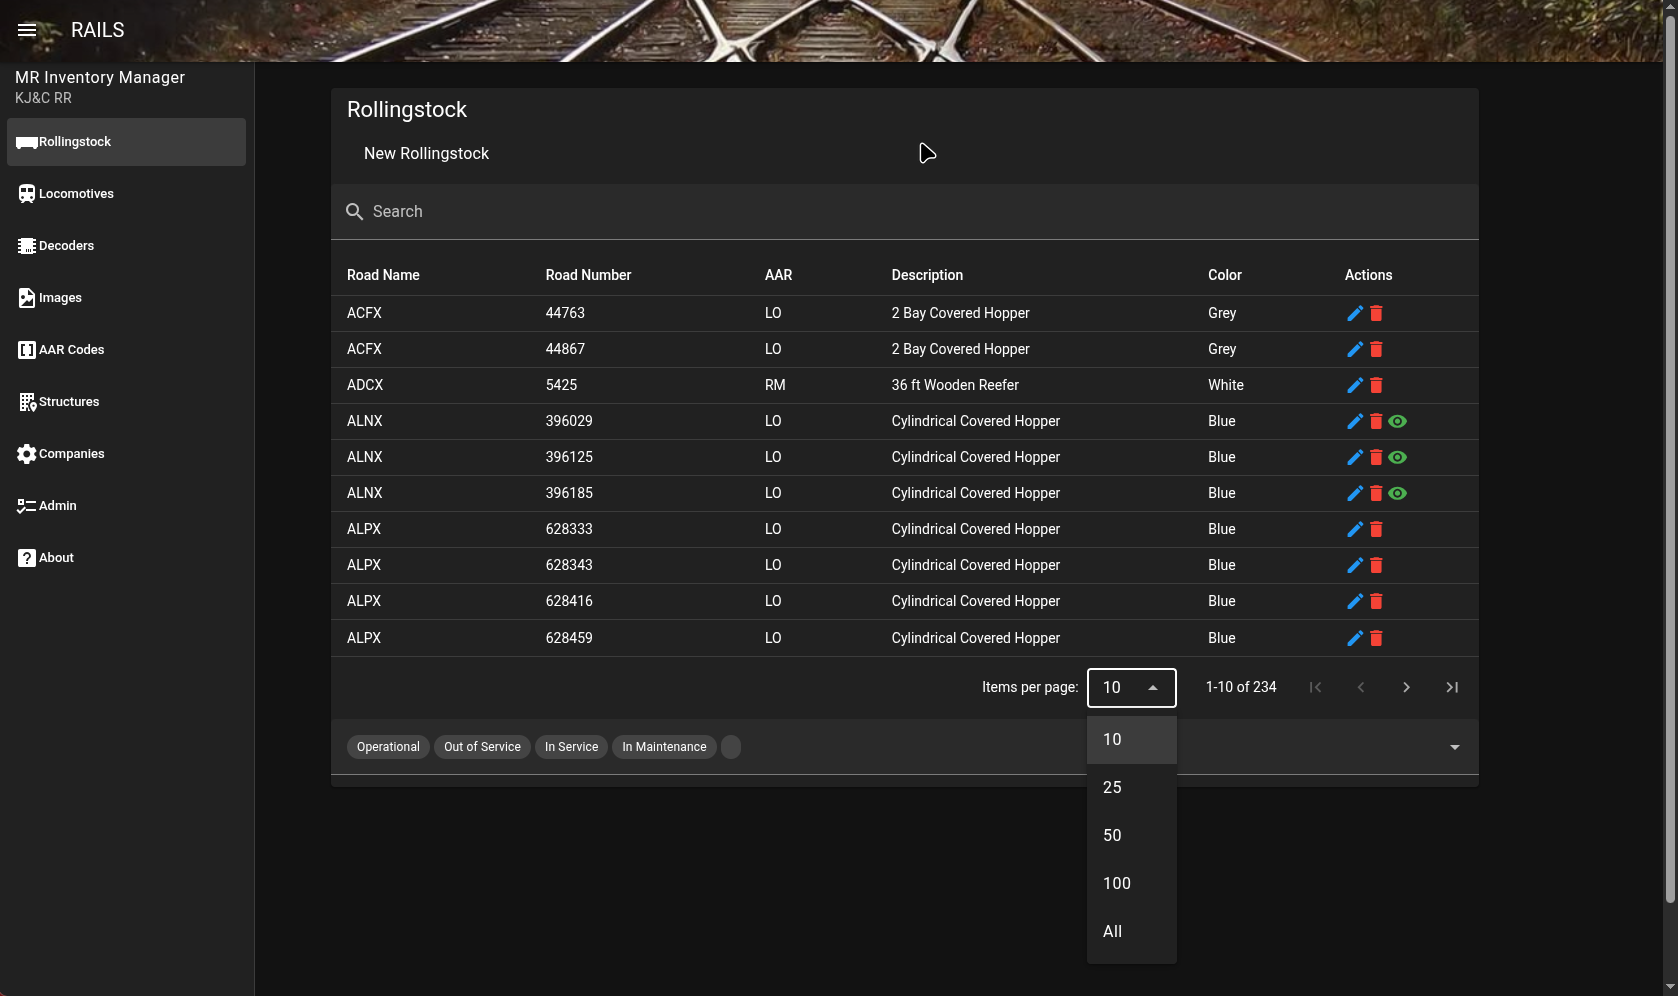
\includegraphics[width=0.85\textwidth]{./images/rs-pg-qty.png}
    \caption{Items Per Page Selection}
    \label{fig:rs-pg-qty}
\end{figure}

\subsection{Status Filtering}

Rolling stock entries can be filtered dynamically based on operational status. At the bottom of the view, status filter controls allow toggling visibility for items designated as Operational, Out of Service, In Service, or In Maintenance. Figure \ref{fig:rs-status} shows the operational status filtering interface open.

\begin{figure}[H]
    \centering
    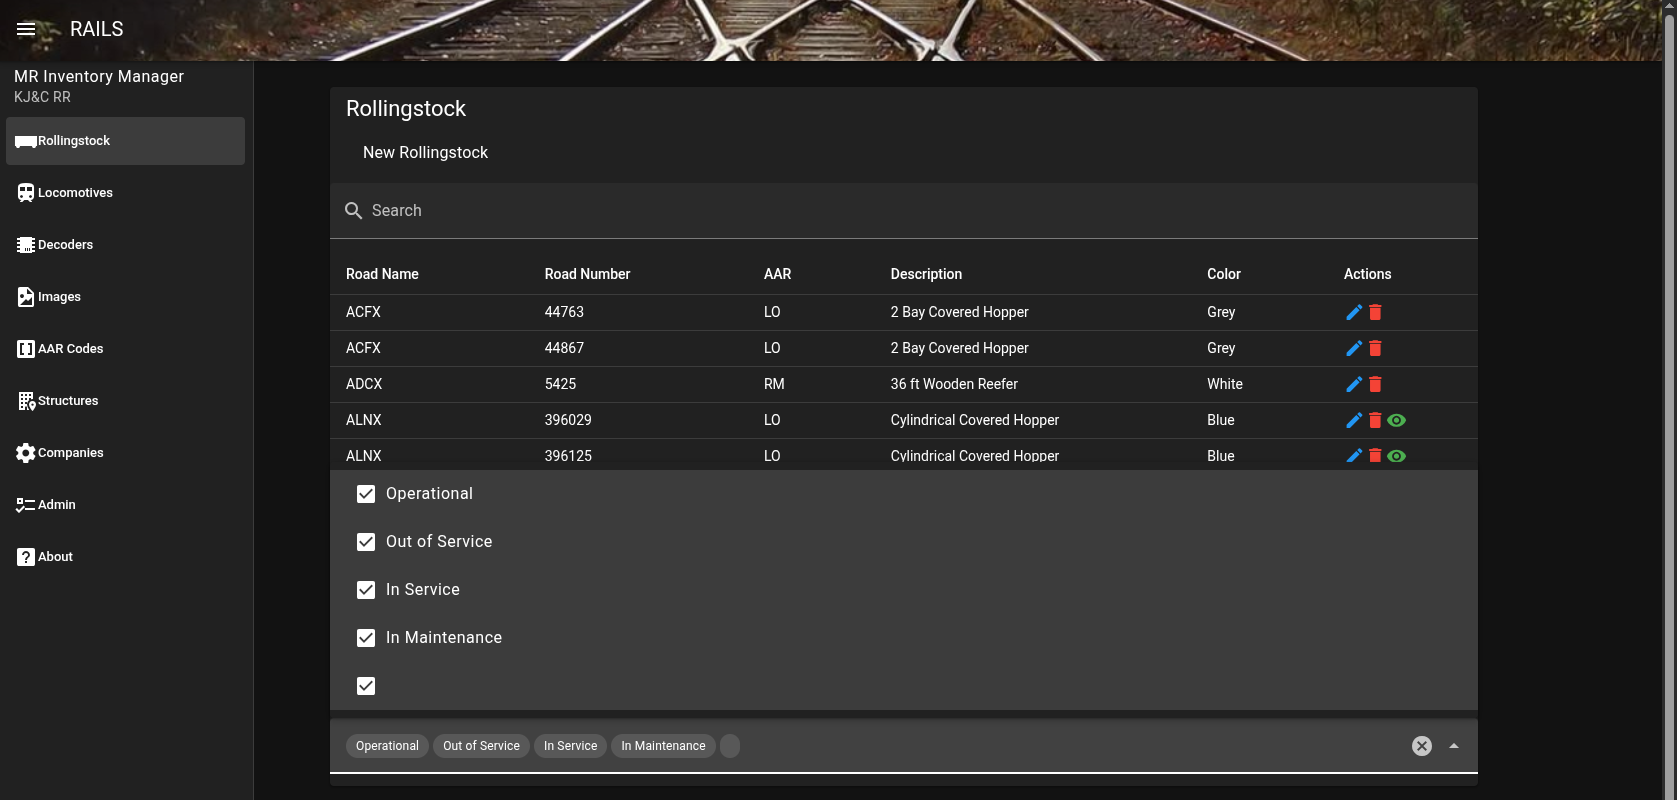
\includegraphics[width=0.85\textwidth]{./images/rs-status.png}
    \caption{Status Filter}
    \label{fig:rs-status}
\end{figure}

\subsection{Search Functionality}

A search bar located above the main table enables real-time filtering across rolling stock attributes. Typing search terms such as a road name (e.g., "cnw") instantly filters the list to show matching records. Figure \ref{fig:rs-search} shows filtered search results.

\begin{figure}[H]
    \centering
    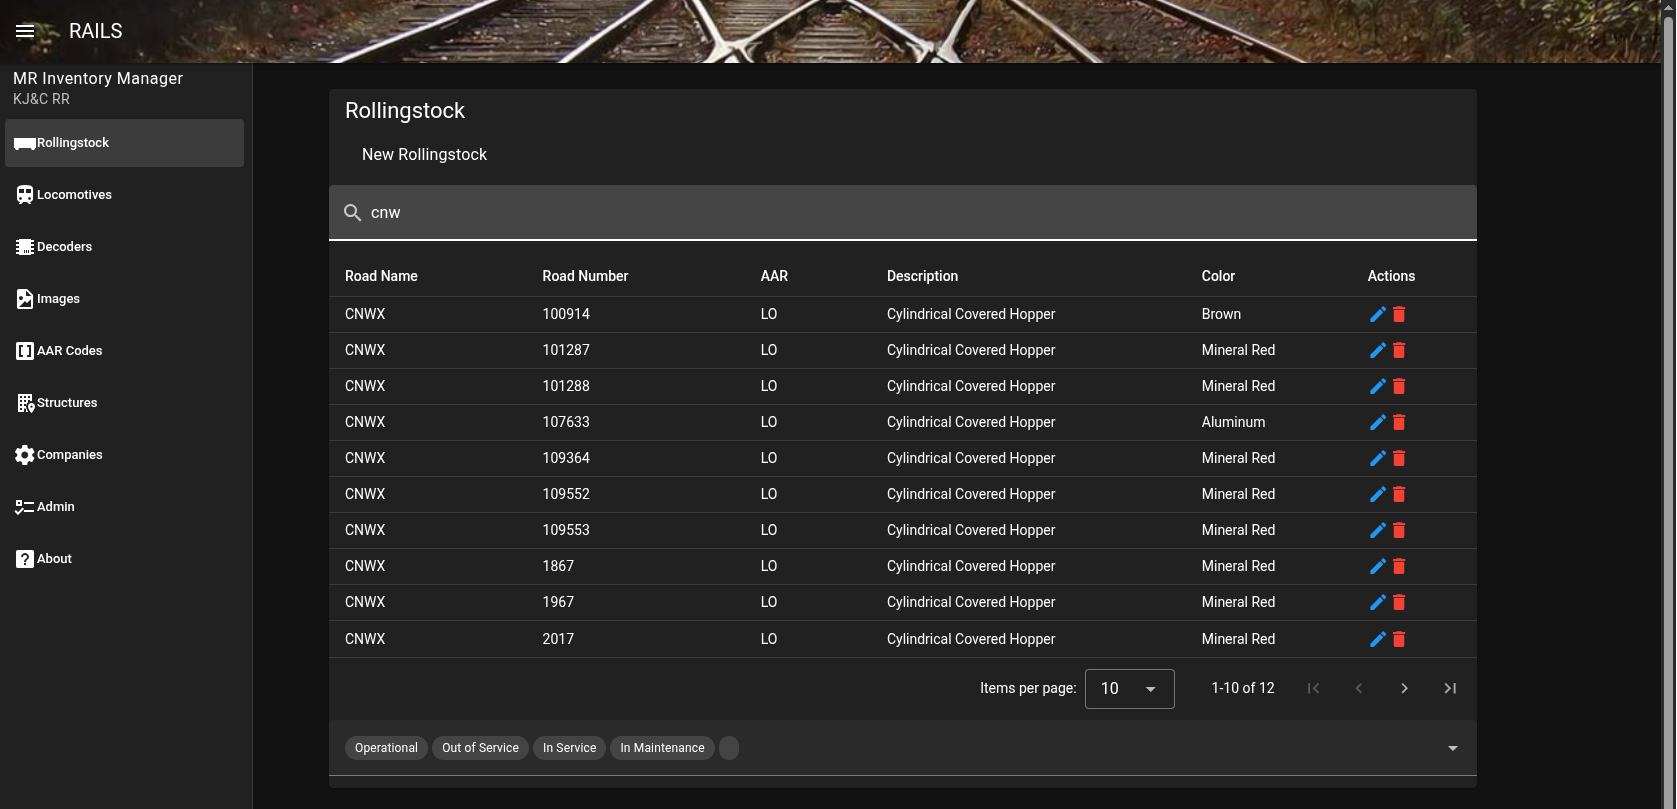
\includegraphics[width=0.85\textwidth]{./images/rs-search.png}
    \caption{Search Rollingstock}
    \label{fig:rs-search}
\end{figure}

\subsection{Viewing Rollingstock Details}

For entries configured with associated image files, an eye icon appears under the Actions column. Clicking this icon opens the Rollingstock Details dialog, displaying comprehensive prototype specifications, dimensions, status, and a photograph of the equipment. Figure \ref{fig:rs-view} shows the detailed view modal for a selected car.

\begin{figure}[H]
    \centering
    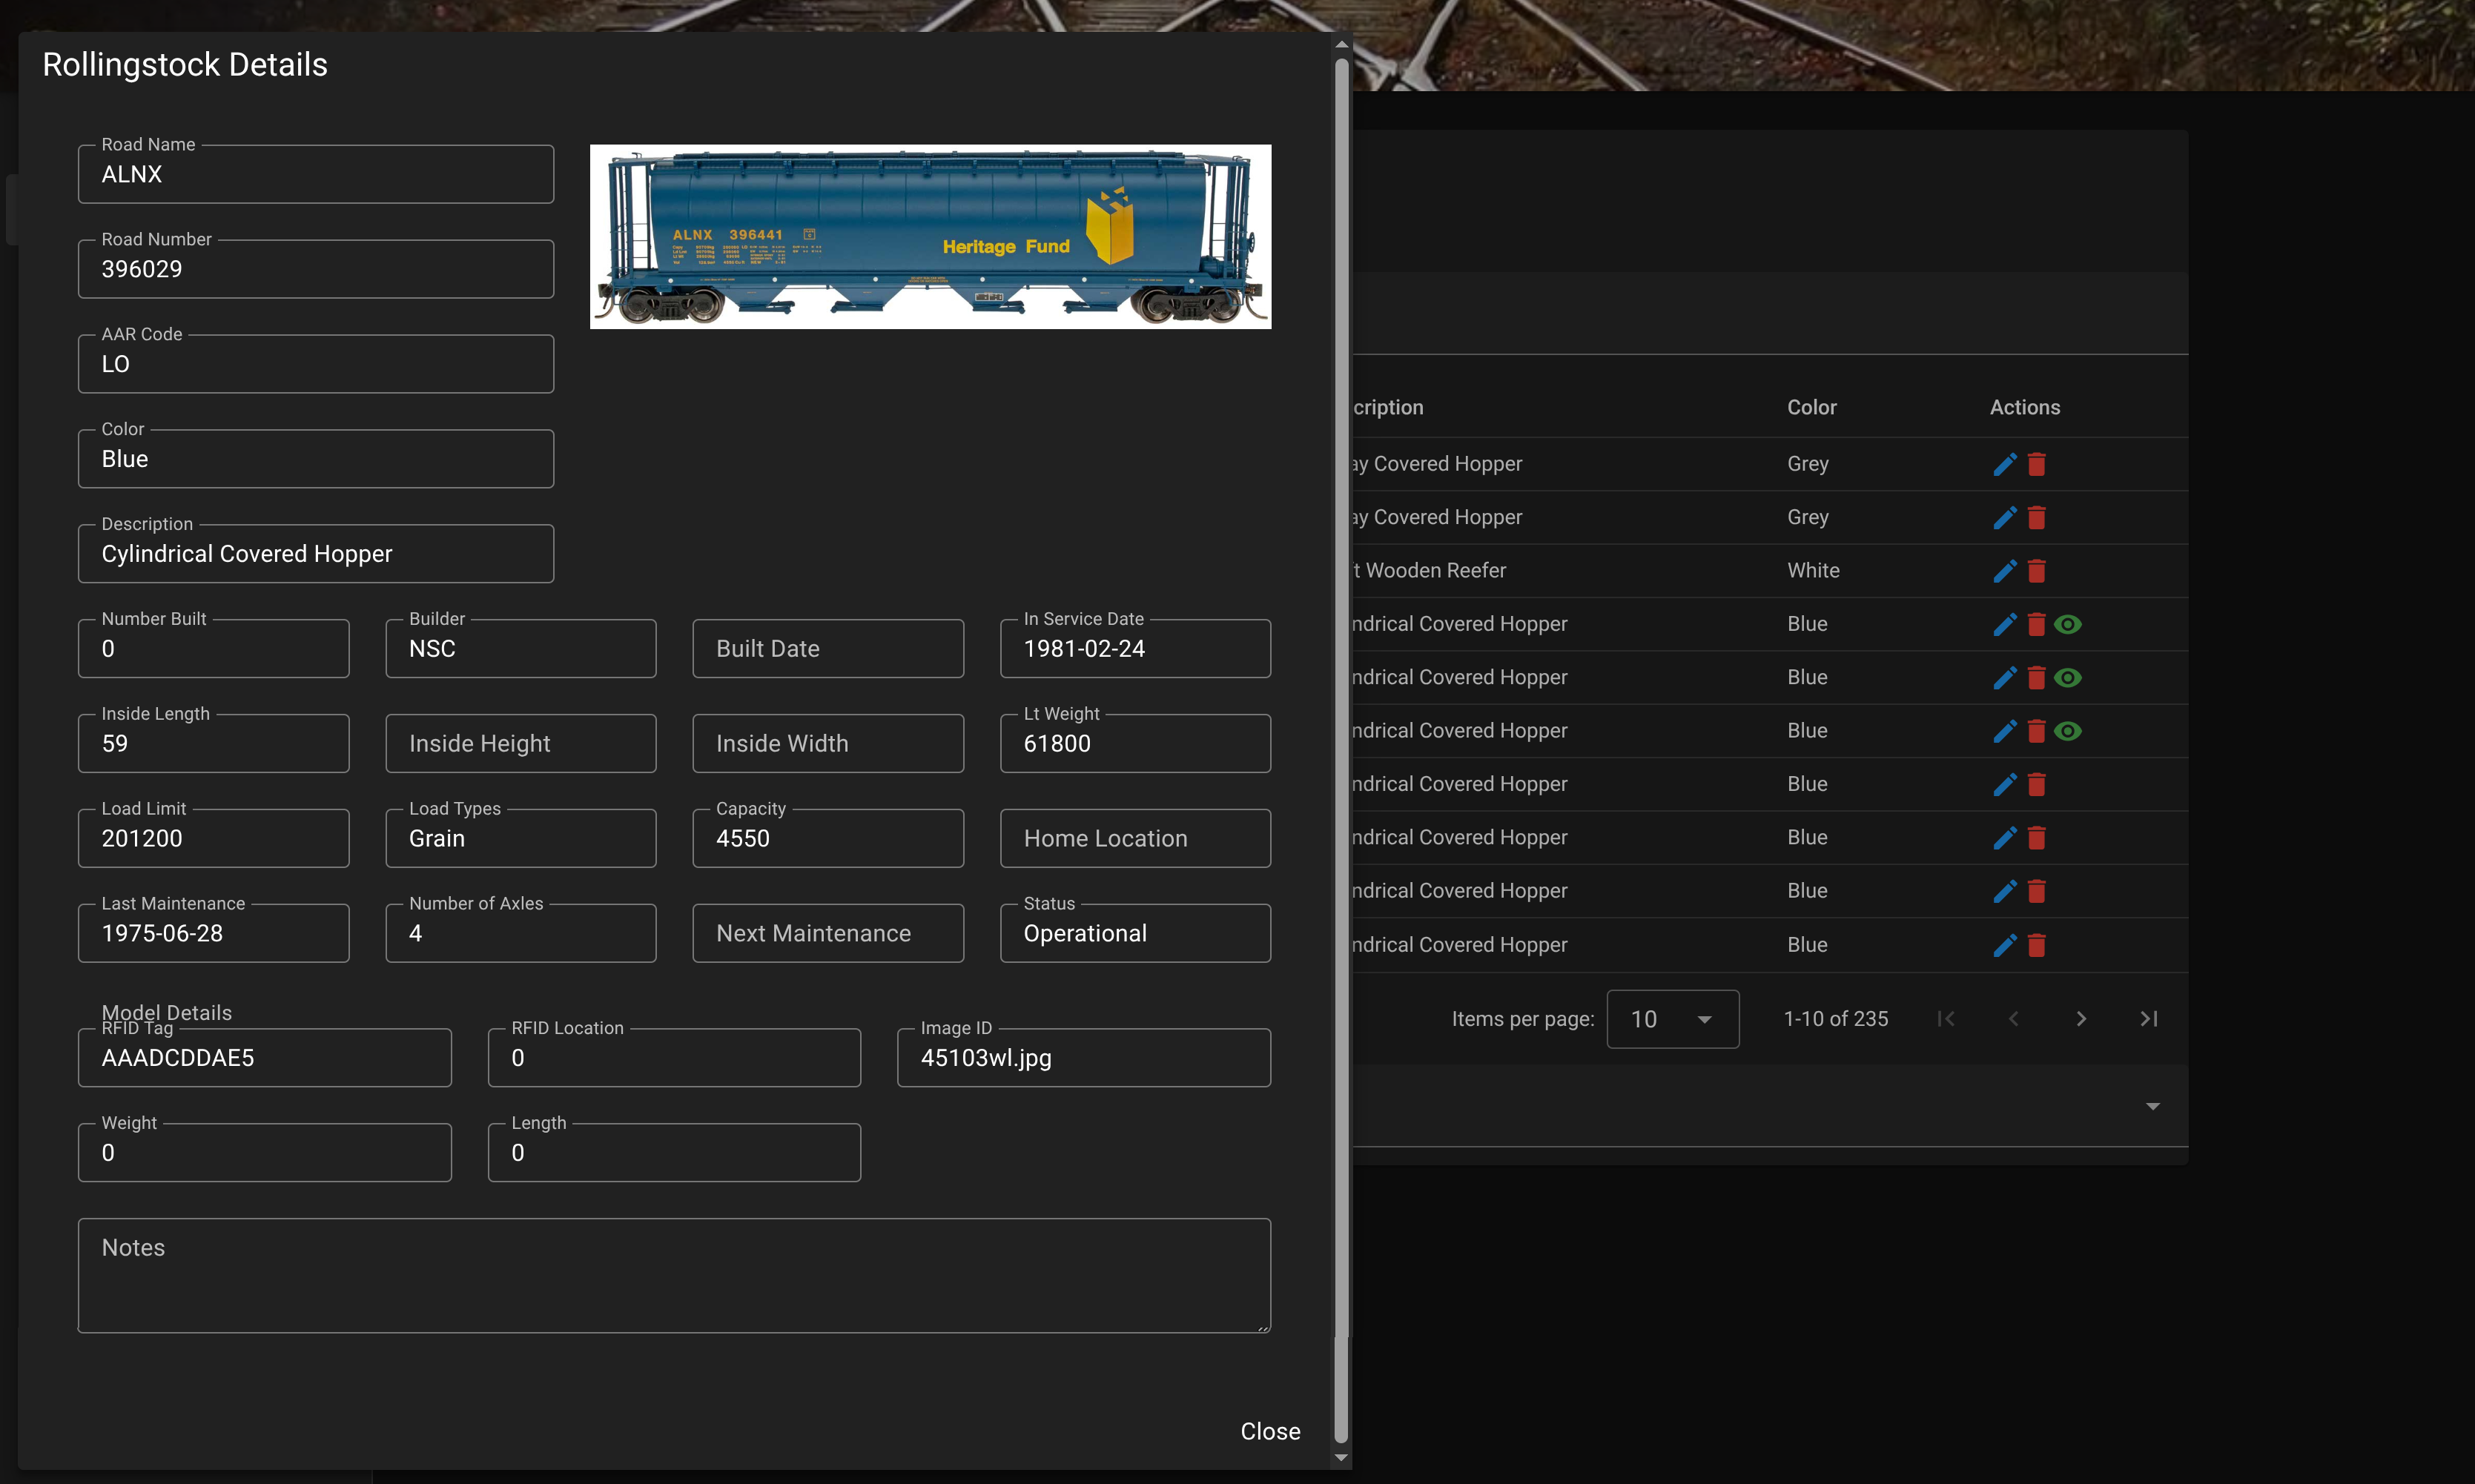
\includegraphics[width=0.85\textwidth]{./images/rs-view.png}
    \caption{View Rollingstock Details}
    \label{fig:rs-view}
\end{figure}

\subsection{Adding New Rollingstock}

Clicking the "New Rollingstock" button above the table opens a blank data entry form. Users can populate fields including road information, dimensions, load characteristics, model parameters, RFID tag associations, and linked image IDs. Figure \ref{fig:rs-new} shows the entry form for creating a new rolling stock item.

\begin{figure}[H]
    \centering
    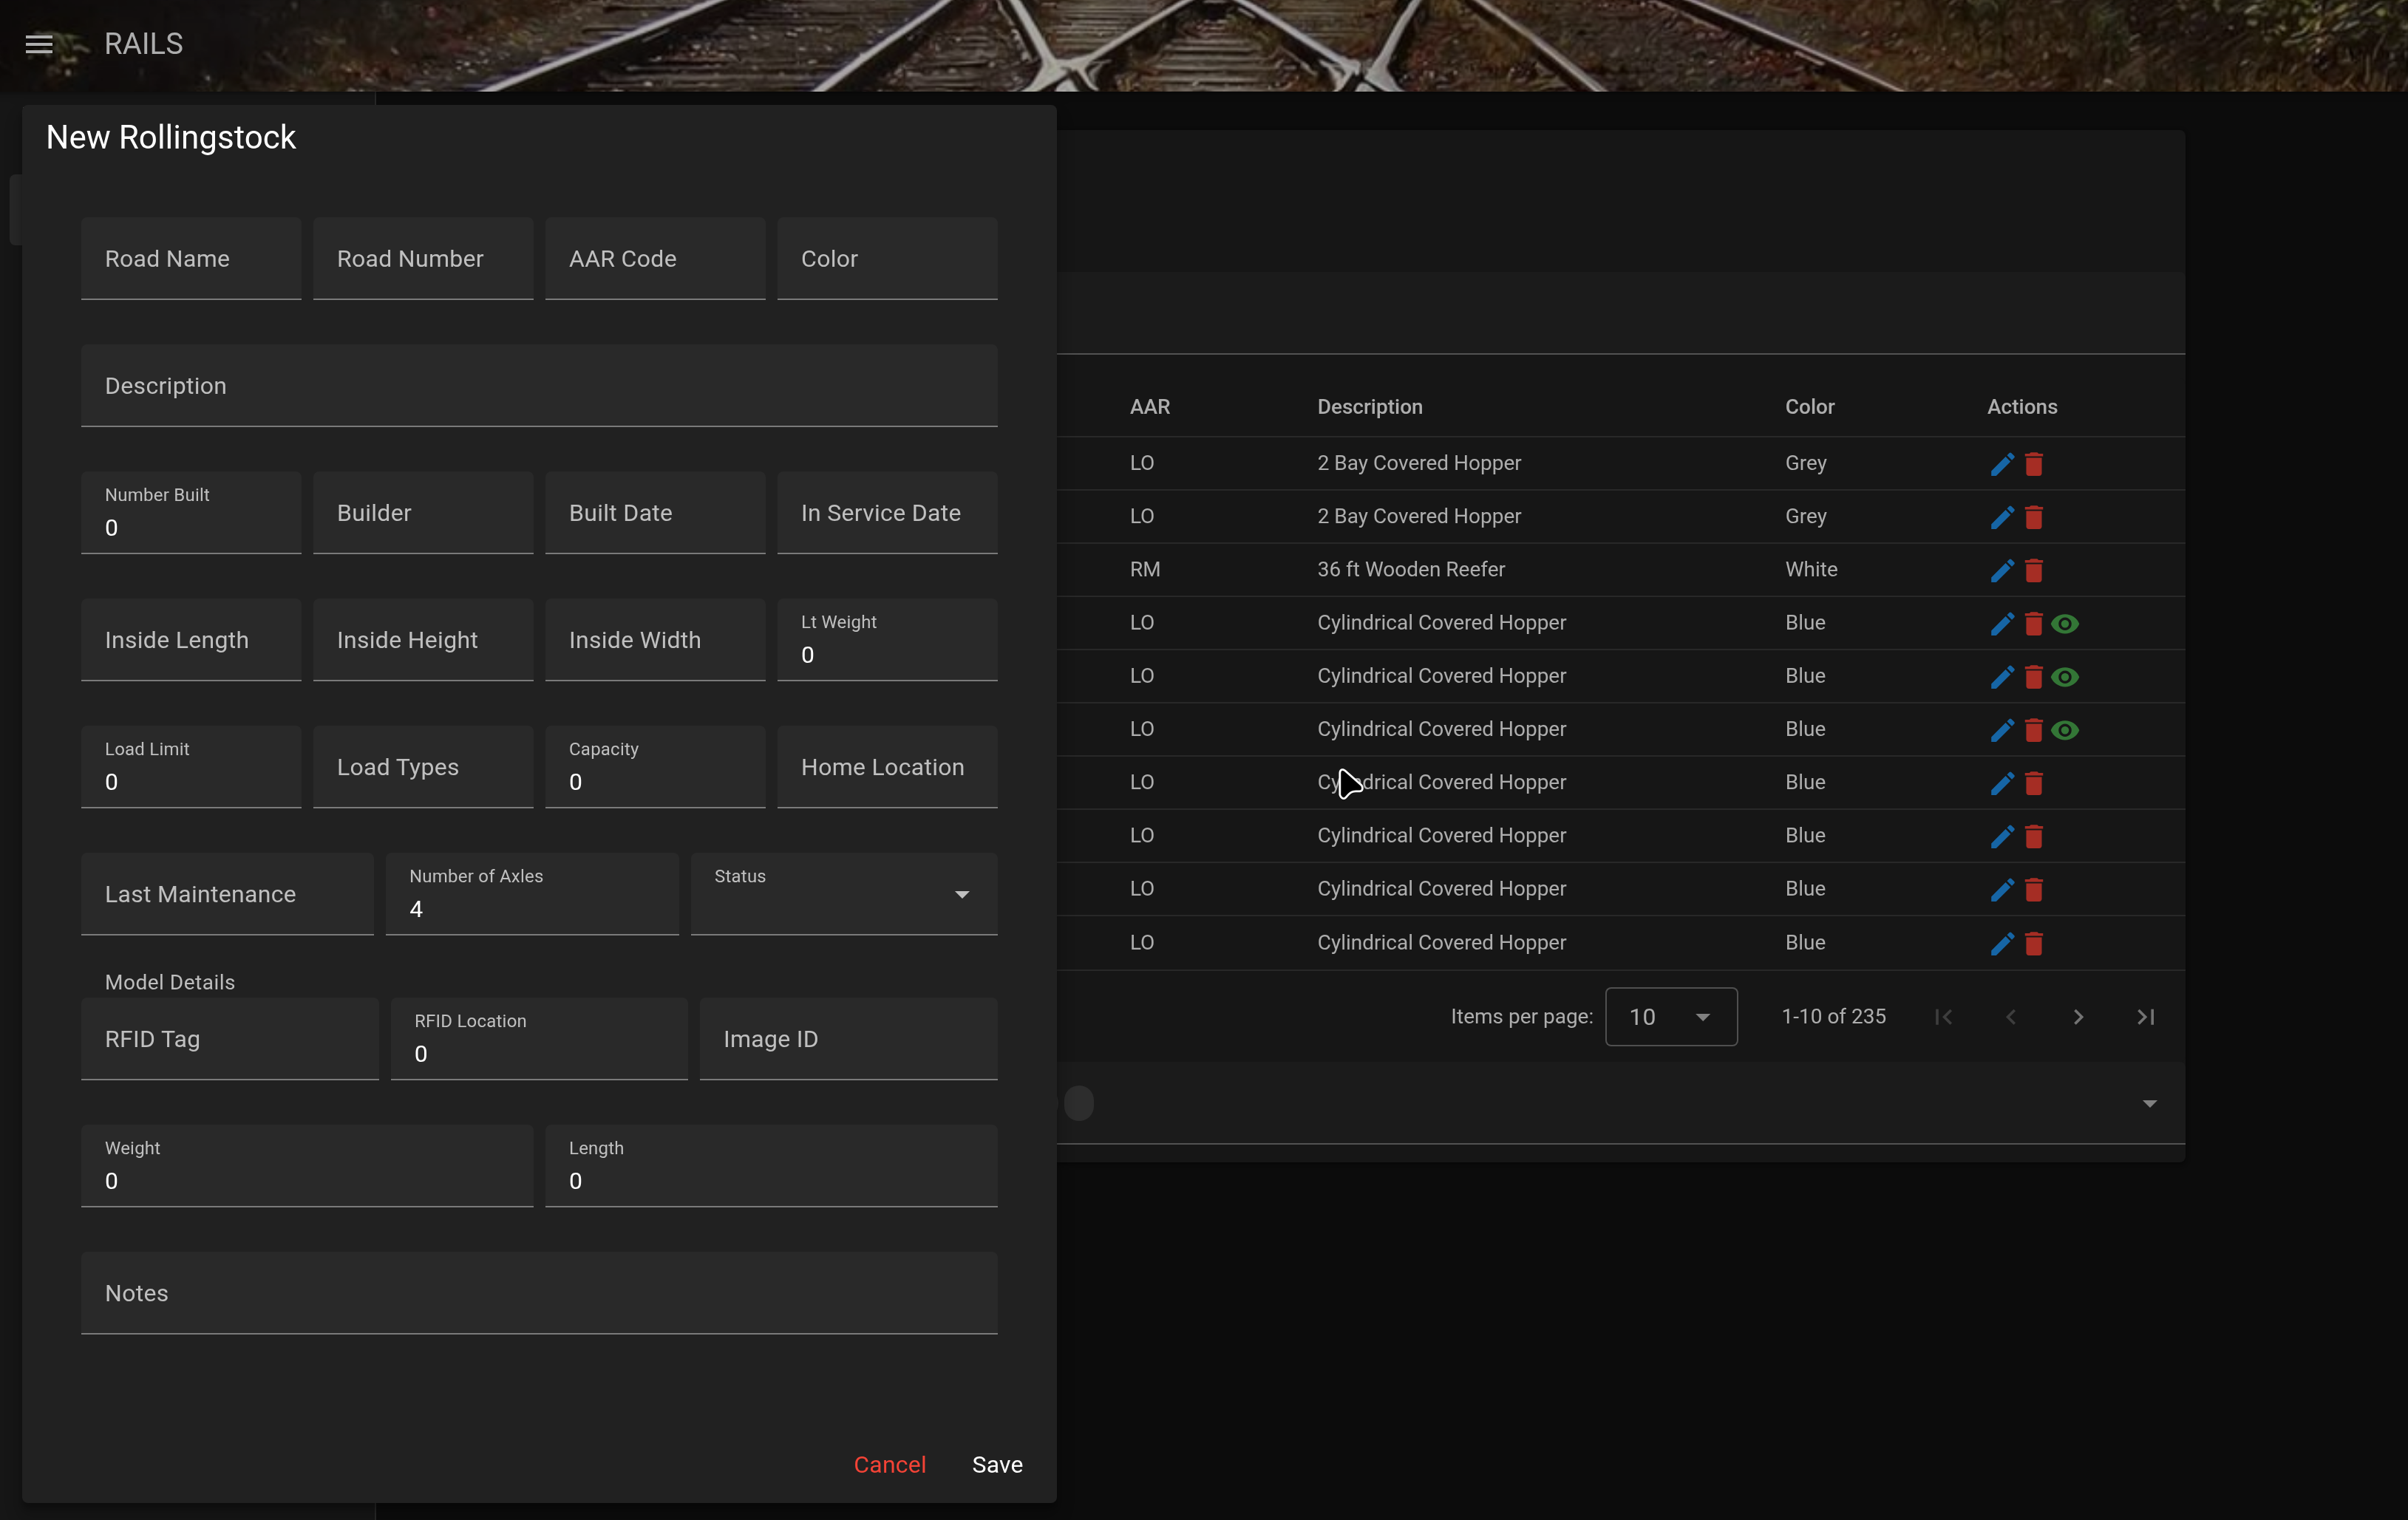
\includegraphics[width=0.85\textwidth]{./images/rs-new.png}
    \caption{New Rollingstock Entry}
    \label{fig:rs-new}
\end{figure}

\subsection{Editing Rollingstock Records}

To modify an existing entry, click the blue pencil icon in the Actions column for that row. This opens the details dialog in editable mode, populated with current record data for updating field values. Figure \ref{fig:rs-edit} illustrates editing an existing record.

\begin{figure}[H]
    \centering
    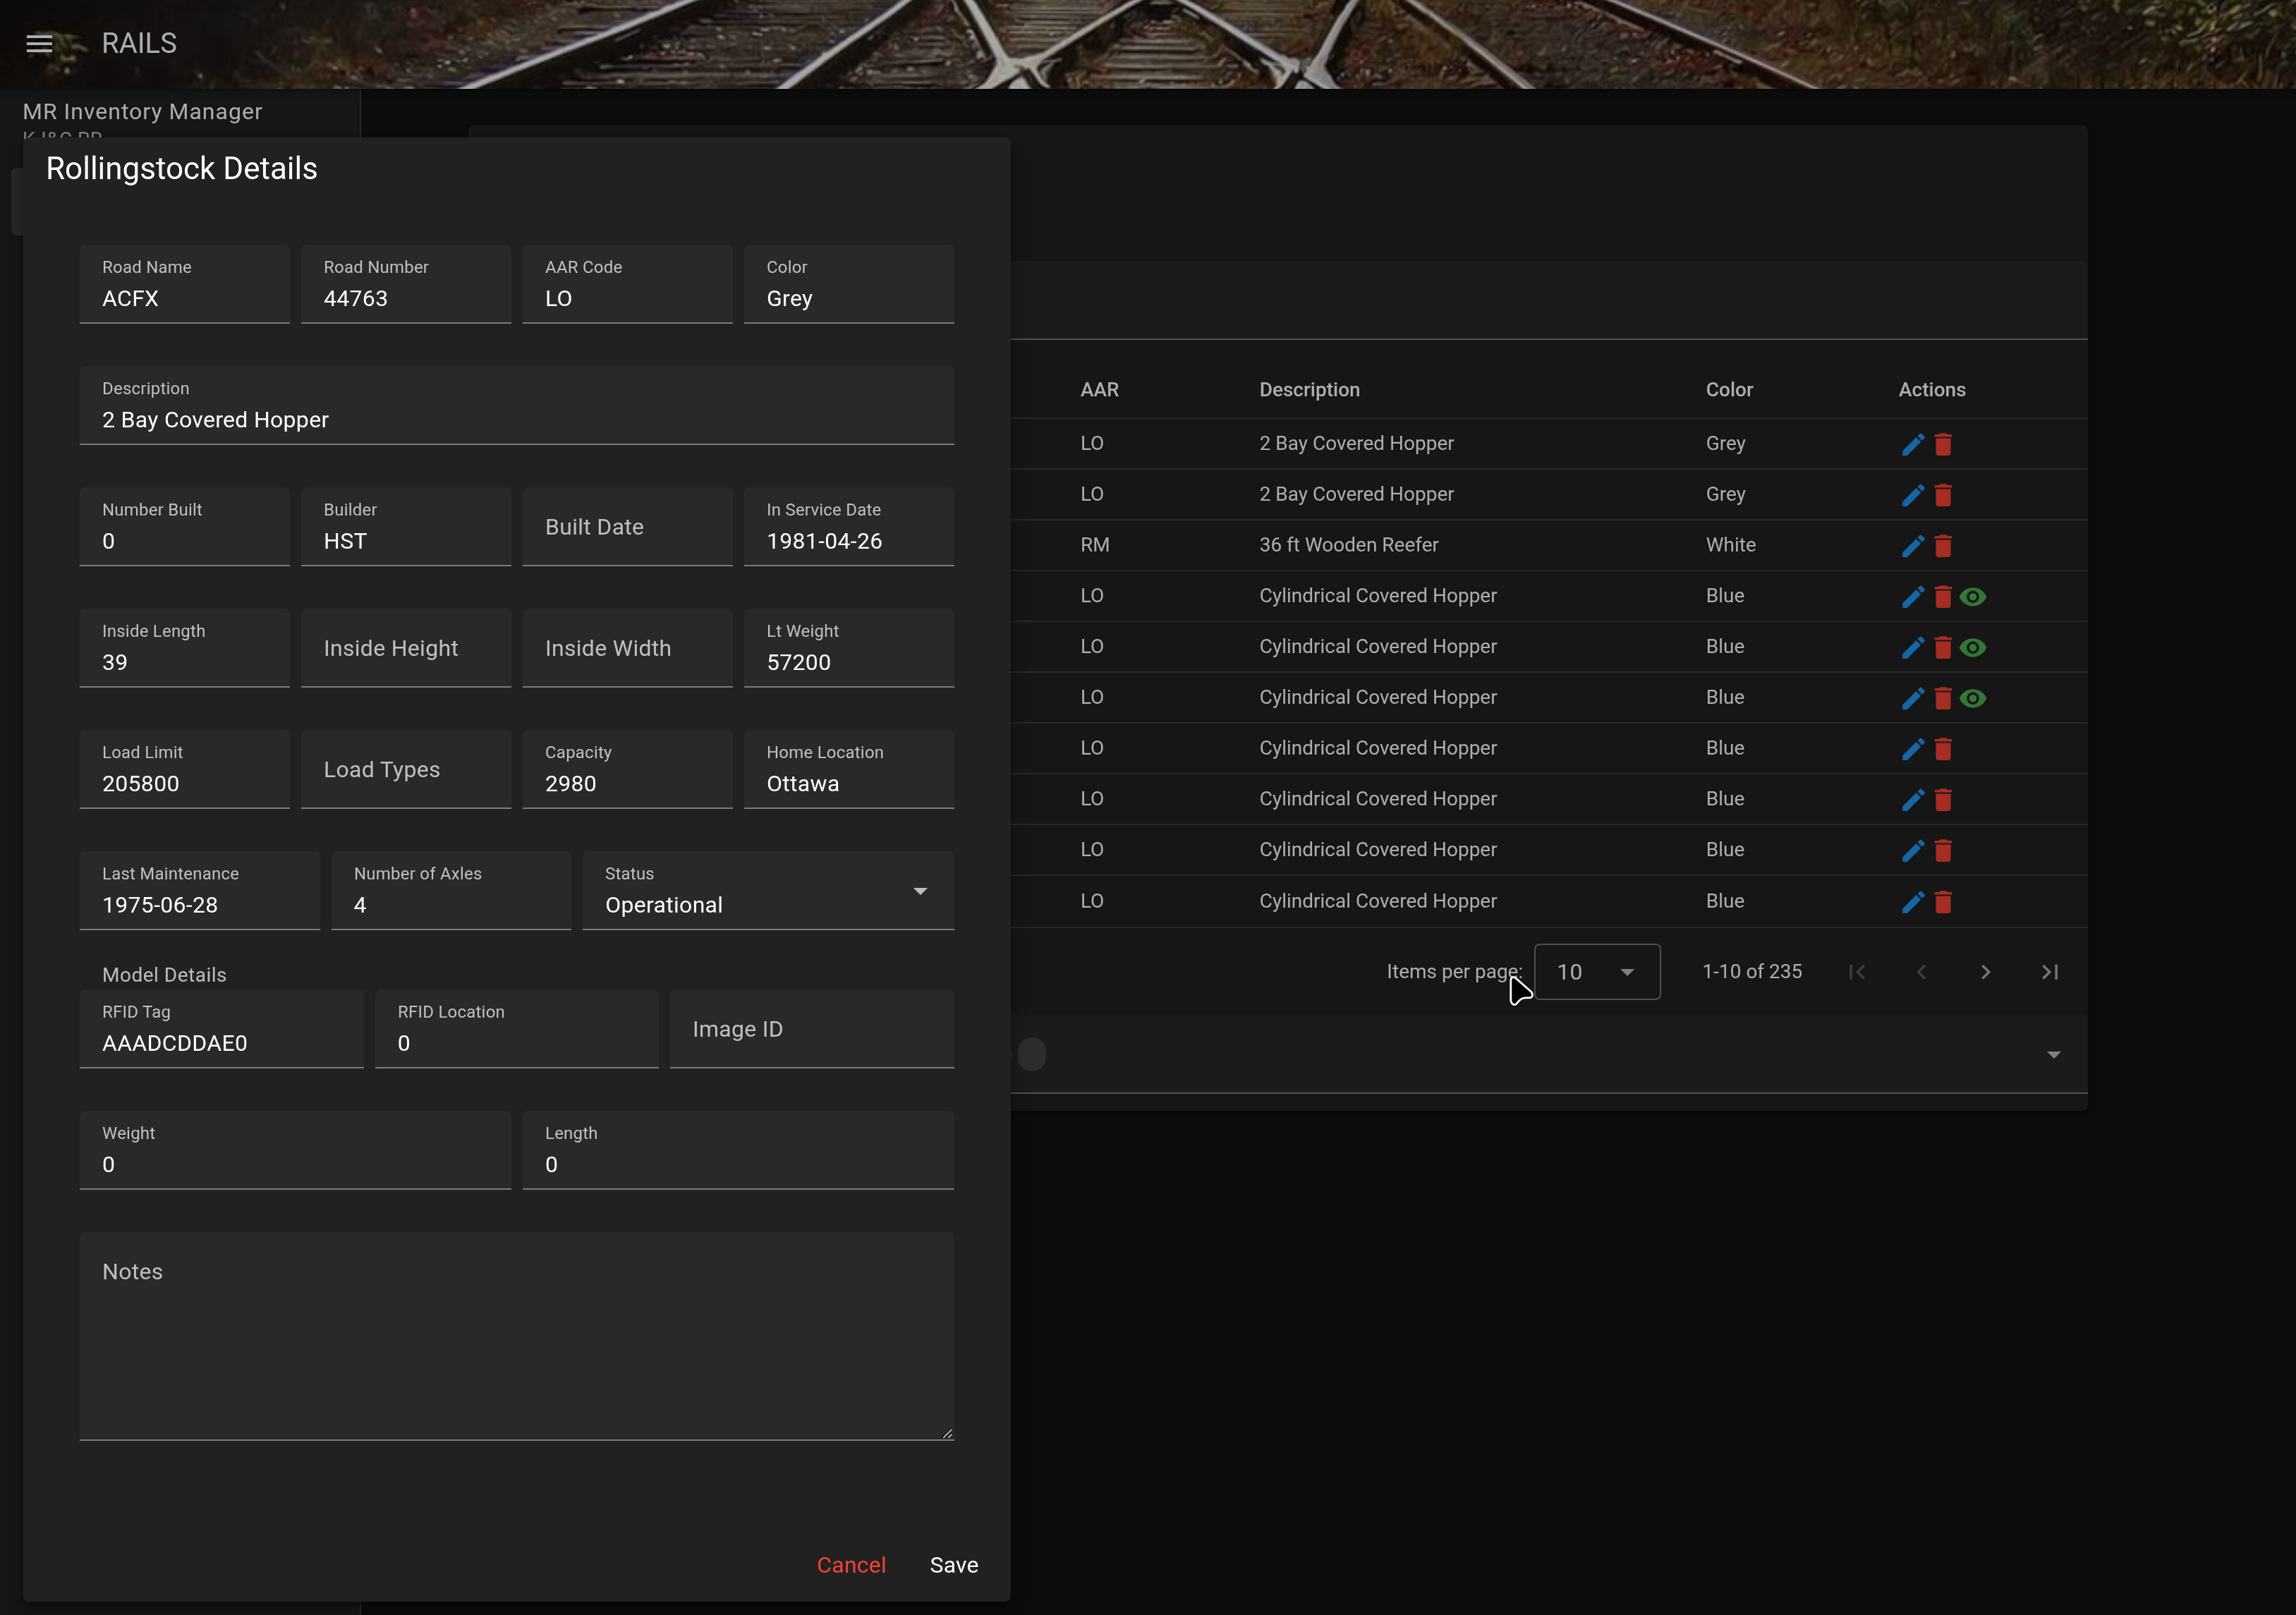
\includegraphics[width=0.85\textwidth]{./images/rs-edit.png}
    \caption{Edit Rollingstock}
    \label{fig:rs-edit}
\end{figure}

\subsection{Deleting Rollingstock Records}

To remove a record from the database, click the red trash bin icon in the Actions column. A confirmation dialog appears requesting confirmation before permanently removing the record. Figure \ref{fig:rs-delete} shows the deletion confirmation prompt.

\begin{figure}[H]
    \centering
    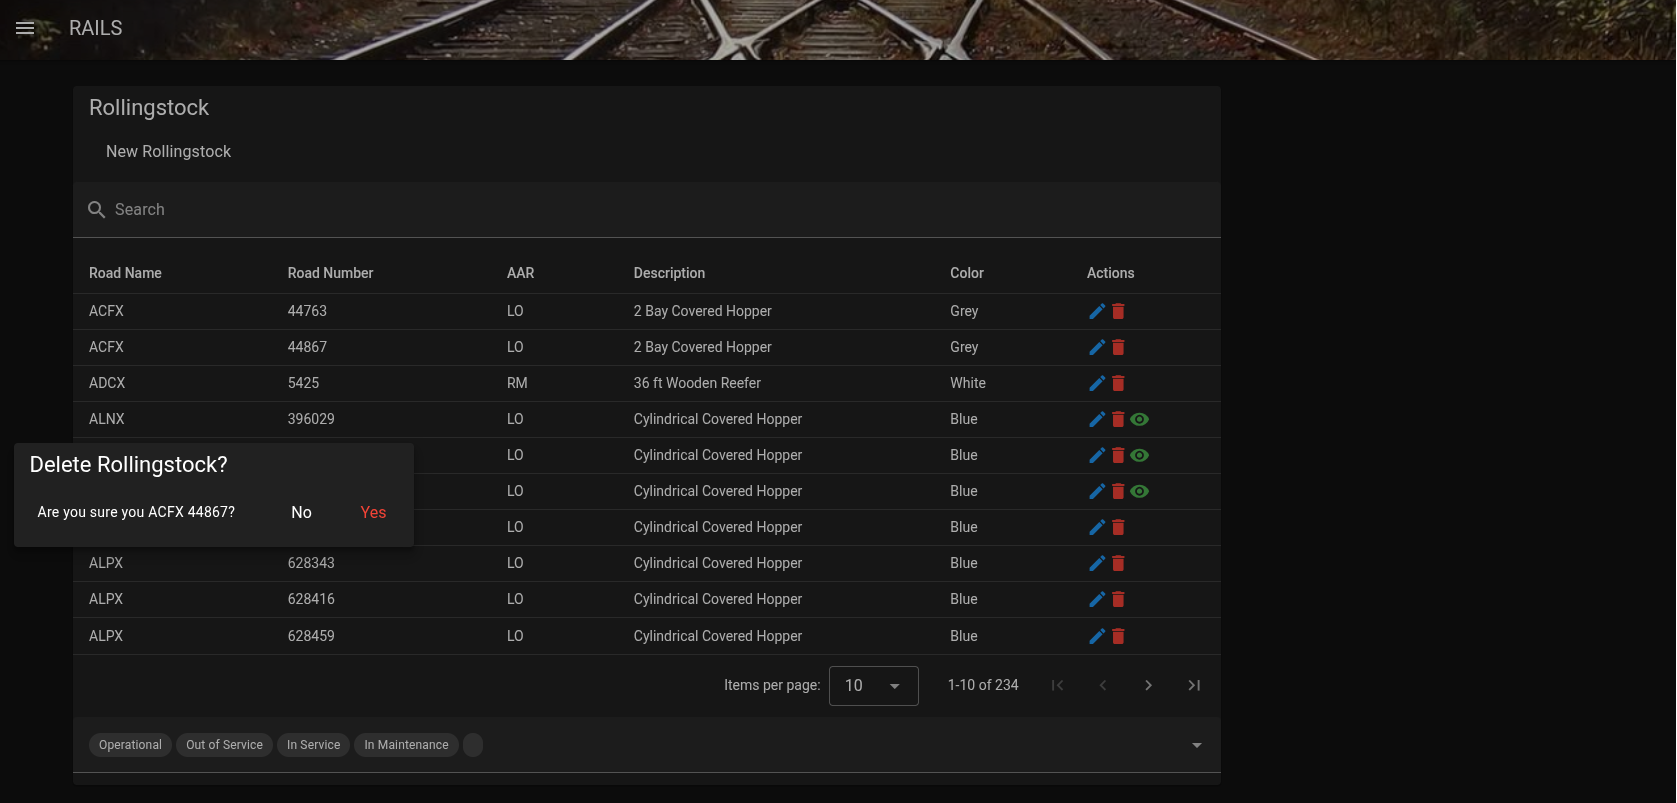
\includegraphics[width=0.85\textwidth]{./images/rs-delete.png}
    \caption{Delete Rollingstock Confirmation}
    \label{fig:rs-delete}
\end{figure}

\section{Locomotives Inventory}

Selecting "Locomotives" from the navigation drawer displays the Inventory of Locomotives view. This table presents a specialized subset of motive power entries from the inventory database, detailing primary attributes such as Road Name, Road Number, AAR designation code, Description, and Color scheme.

\begin{figure}[H]
    \centering
    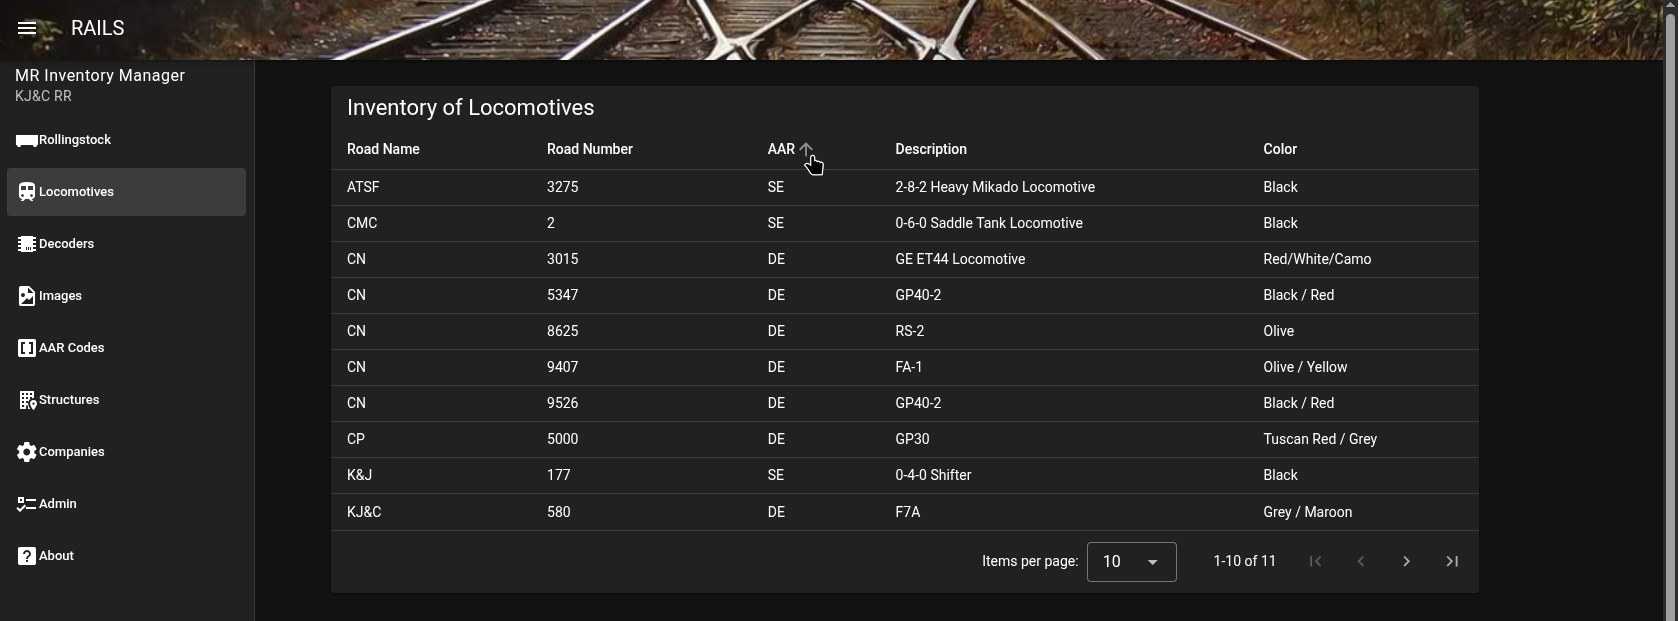
\includegraphics[width=0.85\textwidth]{./images/locos.png}
    \caption{Inventory of Locomotives}
    \label{fig:locos}
\end{figure}

The page incorporates interactive column sorting, as shown by the direction arrow next to the AAR header, allowing motive power records to be ordered by specific attributes. Standard table pagination controls located at the bottom right enable users to adjust the display limit per page and navigate through larger locomotive fleets.

\section{Decoders Management}

Selecting "Decoders" from the navigation drawer displays the main Decoders management view. This page displays a tabular listing of all Digital Command Control (DCC) decoders installed in inventory locomotives, summarizing information such as Road Name, Road Number, Manufacturer, Family, Model, active DCC Address, and available action controls. Figure \ref{fig:decoders} shows the main Decoders table page.

\begin{figure}[H]
    \centering
    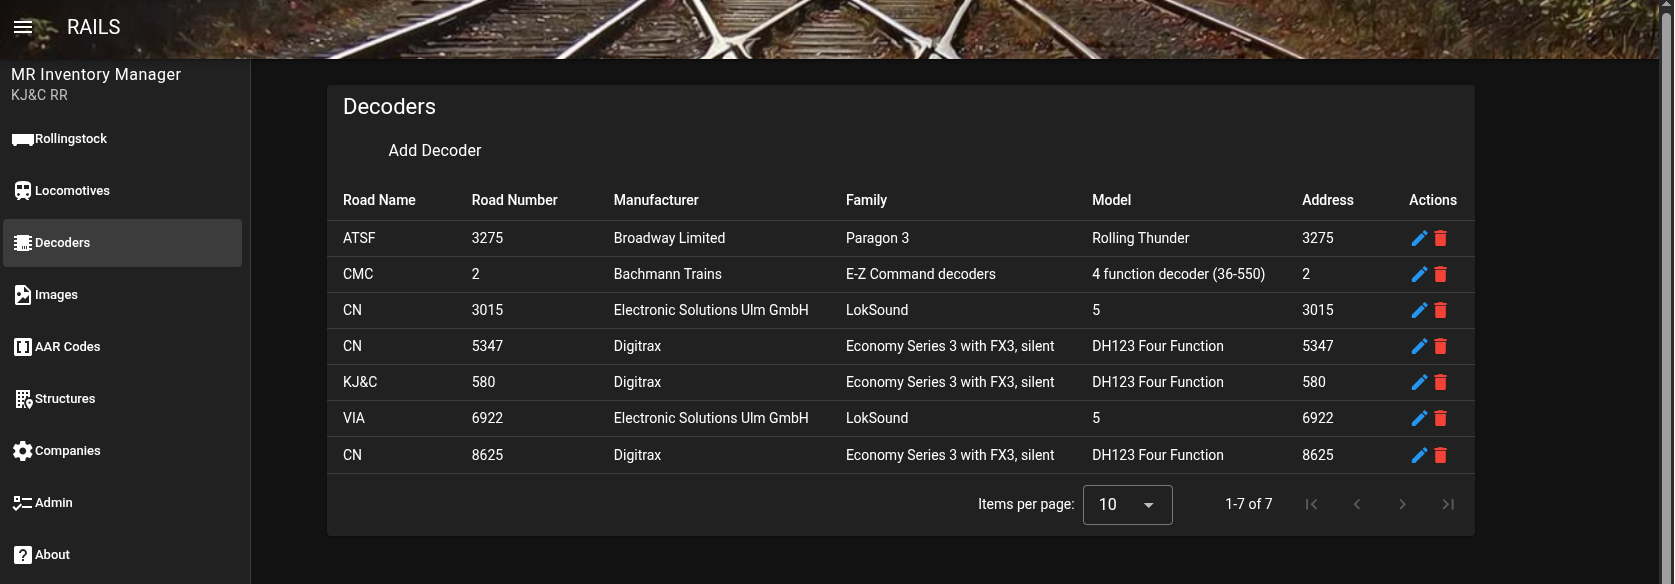
\includegraphics[width=0.85\textwidth]{./images/decoders.png}
    \caption{Decoders Page}
    \label{fig:decoders}
\end{figure}

\subsection{Adding a New Decoder}

Clicking the "Add Decoder" button above the table opens a modal dialog for registering a new decoder entry. The form includes fields for Road Name, Road Number, Manufacturer, Family, Model, and DCC Address. Figure \ref{fig:decoders-new} shows the new decoder entry dialog.

\begin{figure}[H]
    \centering
    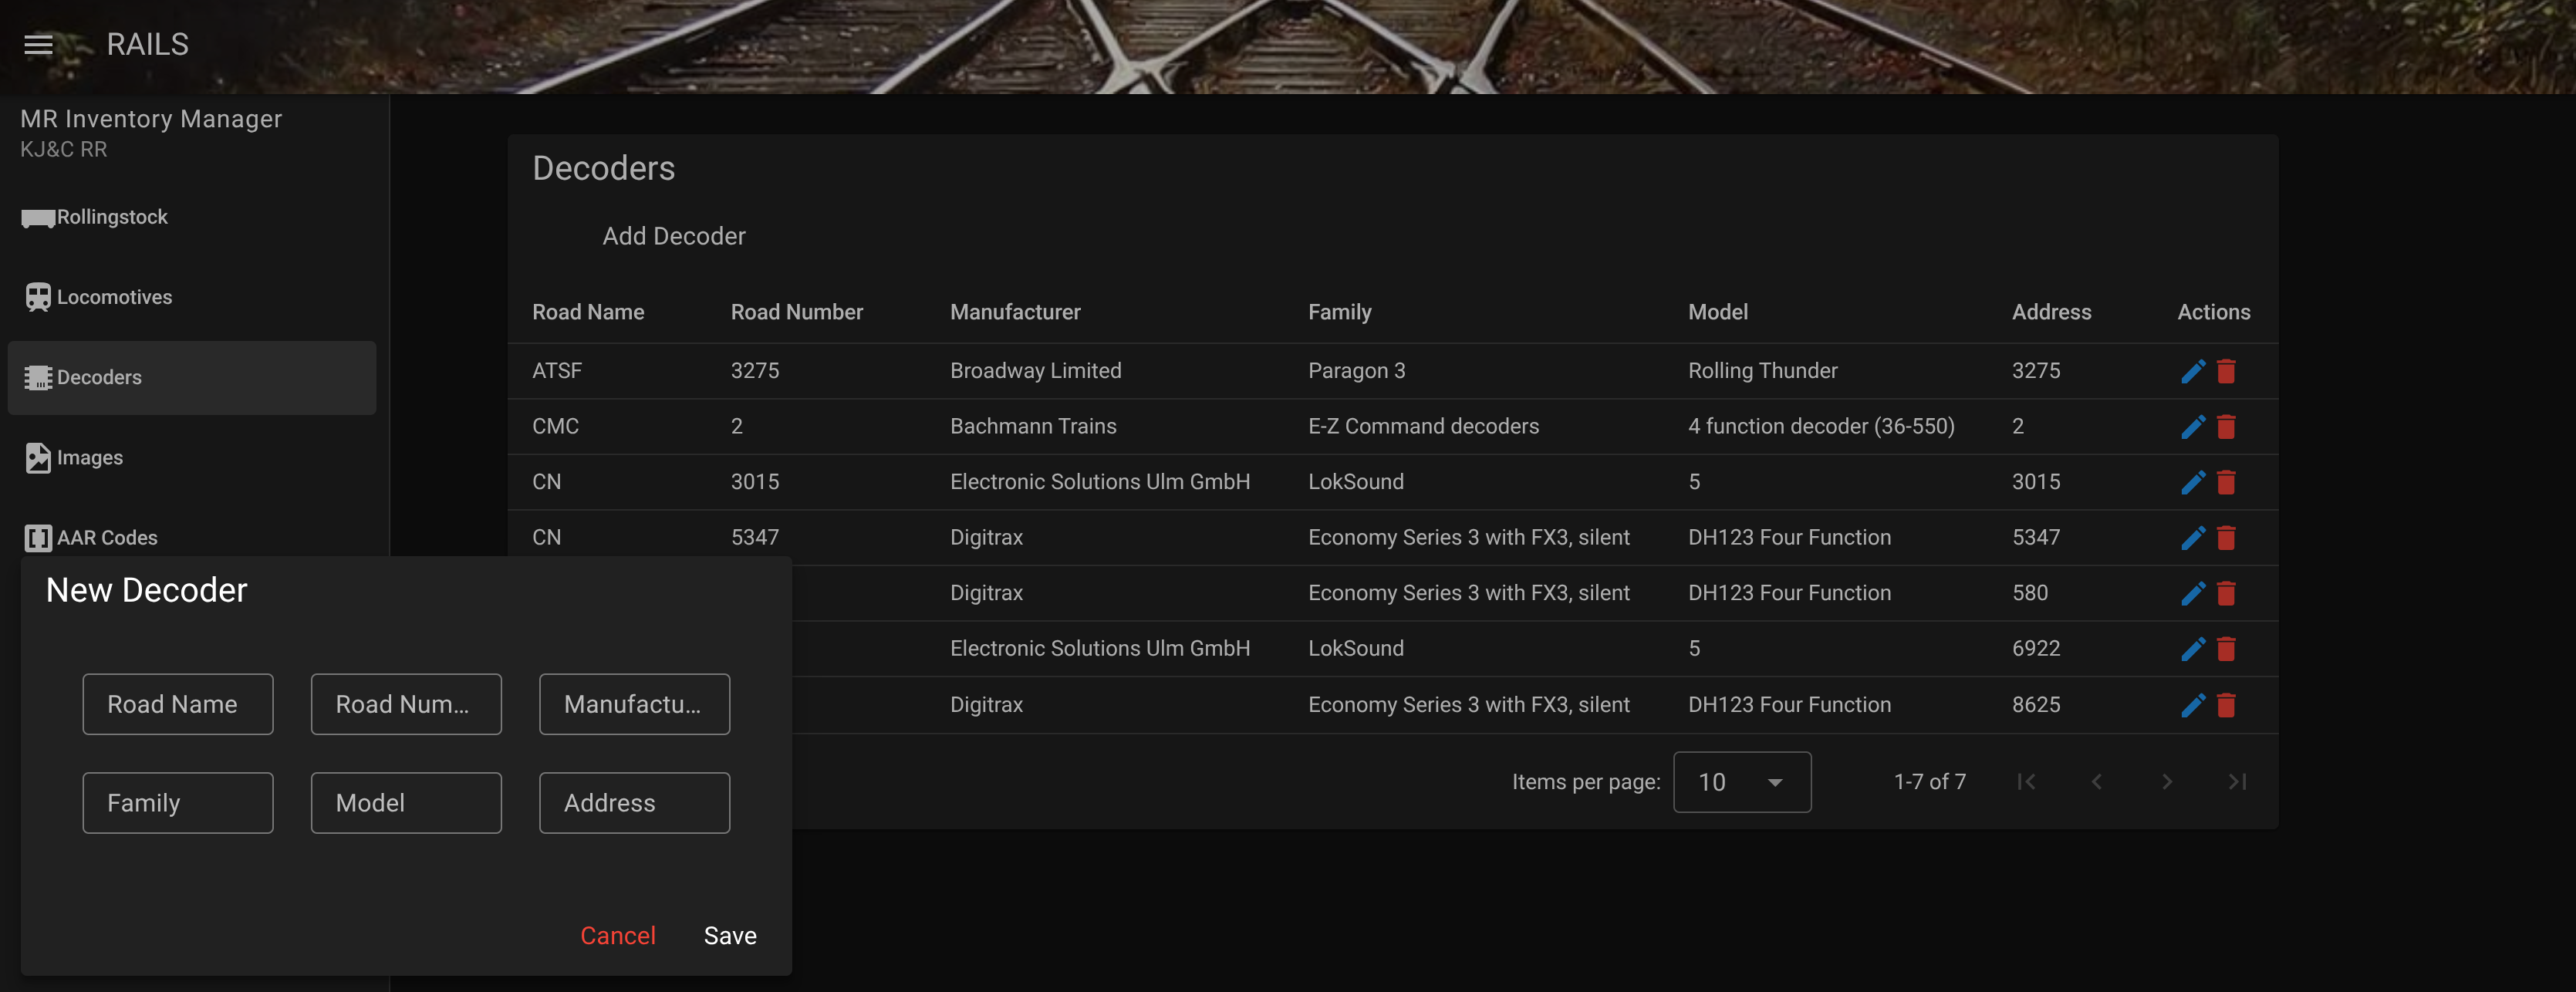
\includegraphics[width=0.85\textwidth]{./images/decoders-new.png}
    \caption{Add Decoder}
    \label{fig:decoders-new}
\end{figure}

\subsection{Editing Decoder Records}

To modify an existing decoder entry, click the blue pencil icon under the Actions column. This opens the decoder configuration form pre-populated with current settings, allowing updates to hardware details or DCC address assignments. Figure \ref{fig:decoders-edit} displays the edit decoder interface.

\begin{figure}[H]
    \centering
    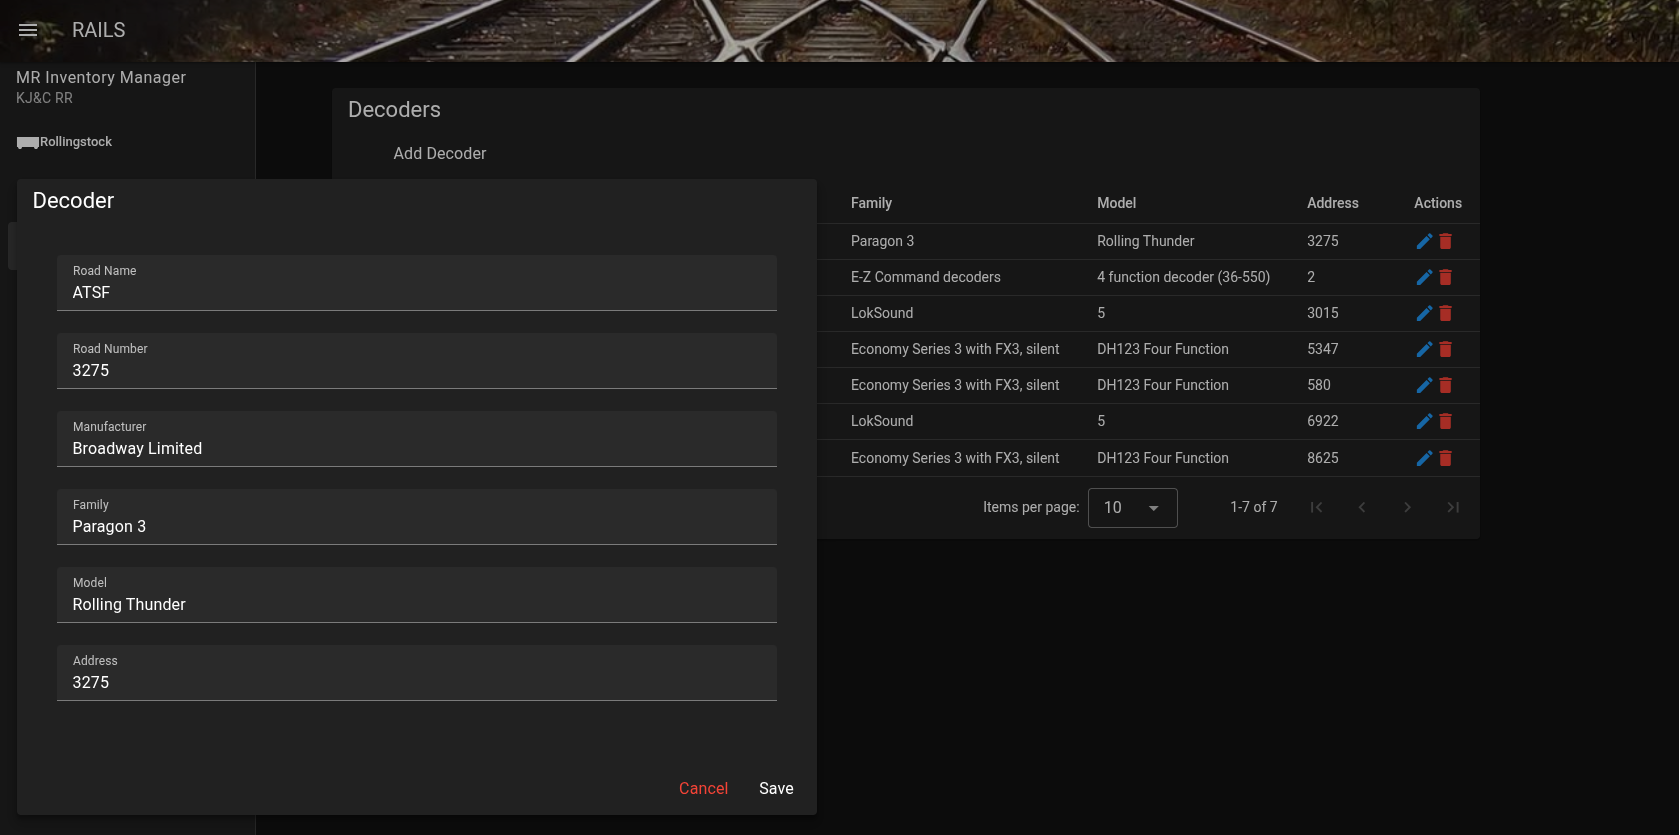
\includegraphics[width=0.85\textwidth]{./images/decoders-edit.png}
    \caption{Edit Decoder}
    \label{fig:decoders-edit}
\end{figure}

\subsection{Deleting Decoder Records}

To delete a decoder entry, click the red trash bin icon in the Actions column. A modal confirmation prompt appears requesting verification before the record is permanently removed from the database. Figure \ref{fig:decoders-delete} illustrates the deletion confirmation dialog.

\begin{figure}[H]
    \centering
    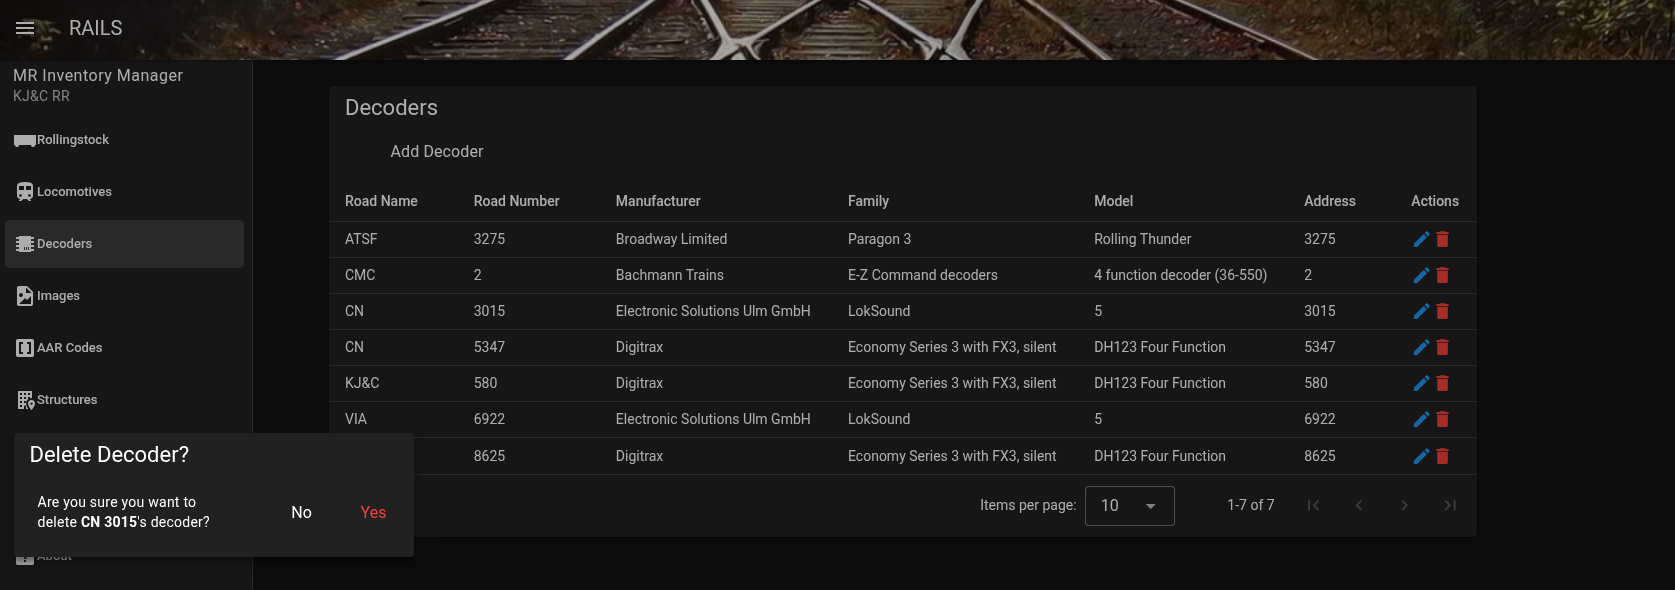
\includegraphics[width=0.85\textwidth]{./images/decoders-delete.png}
    \caption{Delete Decoder Confirmation}
    \label{fig:decoders-delete}
\end{figure}

\section{Image Management}

Selecting "Images" from the navigation drawer displays the Images management viewimages. This page displays a tabular repository of all uploaded graphic assets stored in the Model Railroad File Manager (MRFM) microserviceimages, detailing each item's Title, File Name, assigned Category (e.g., Rollingstock or Structure), and Action buttonsimages. Figure \ref{fig:images} shows the main Images view.

\begin{figure}[H]
    \centering
    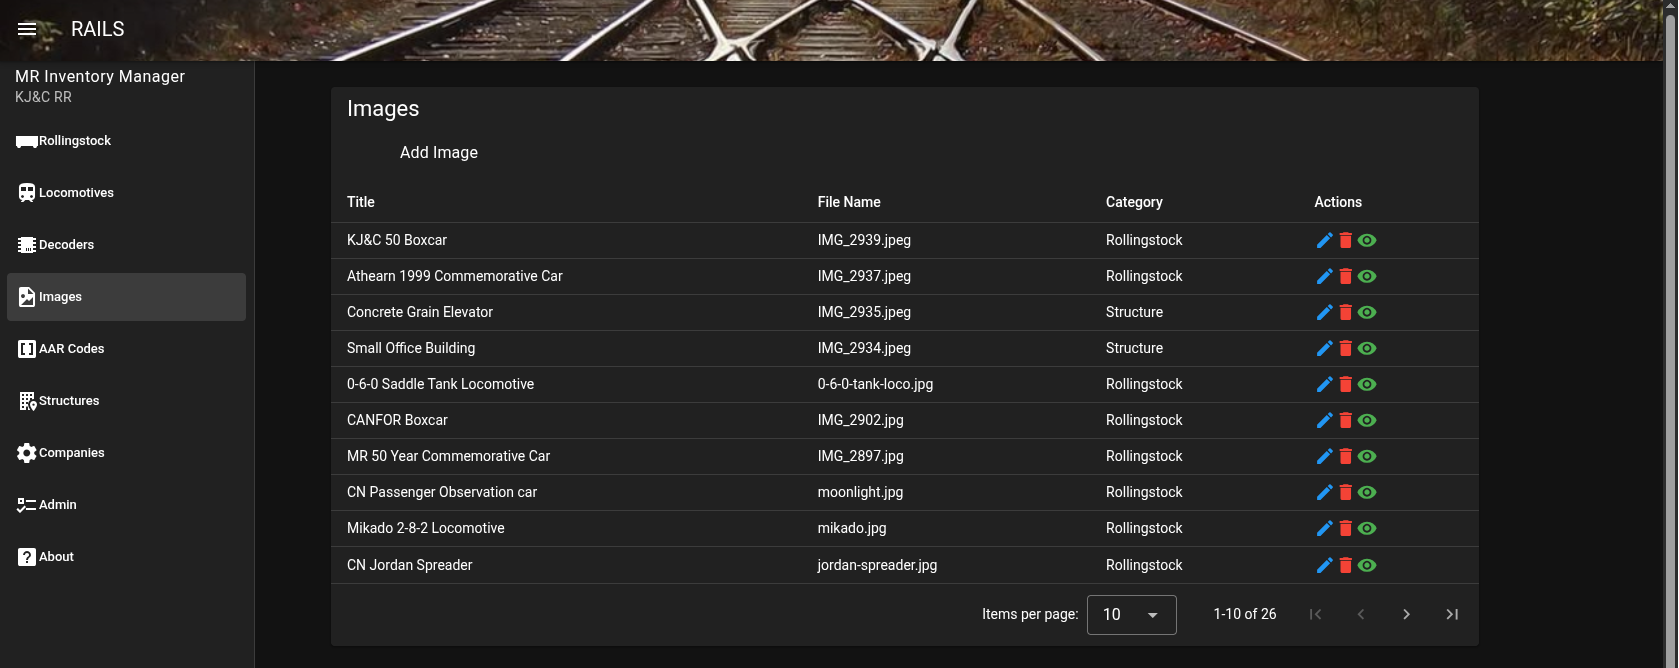
\includegraphics[width=0.85\textwidth]{./images/images.png}
    \caption{Images Page}
    \label{fig:images}
\end{figure}

\subsection{Viewing Image Details}

Clicking the green eye icon under the Actions column opens a modal dialog showing full metadata and a visual preview of the selected assetimages. The dialog presents the Title, File Name, Category, optional Notes, and an embedded image preview. Figure \ref{fig:images-view} shows the image viewer dialog.

\begin{figure}[H]
    \centering
    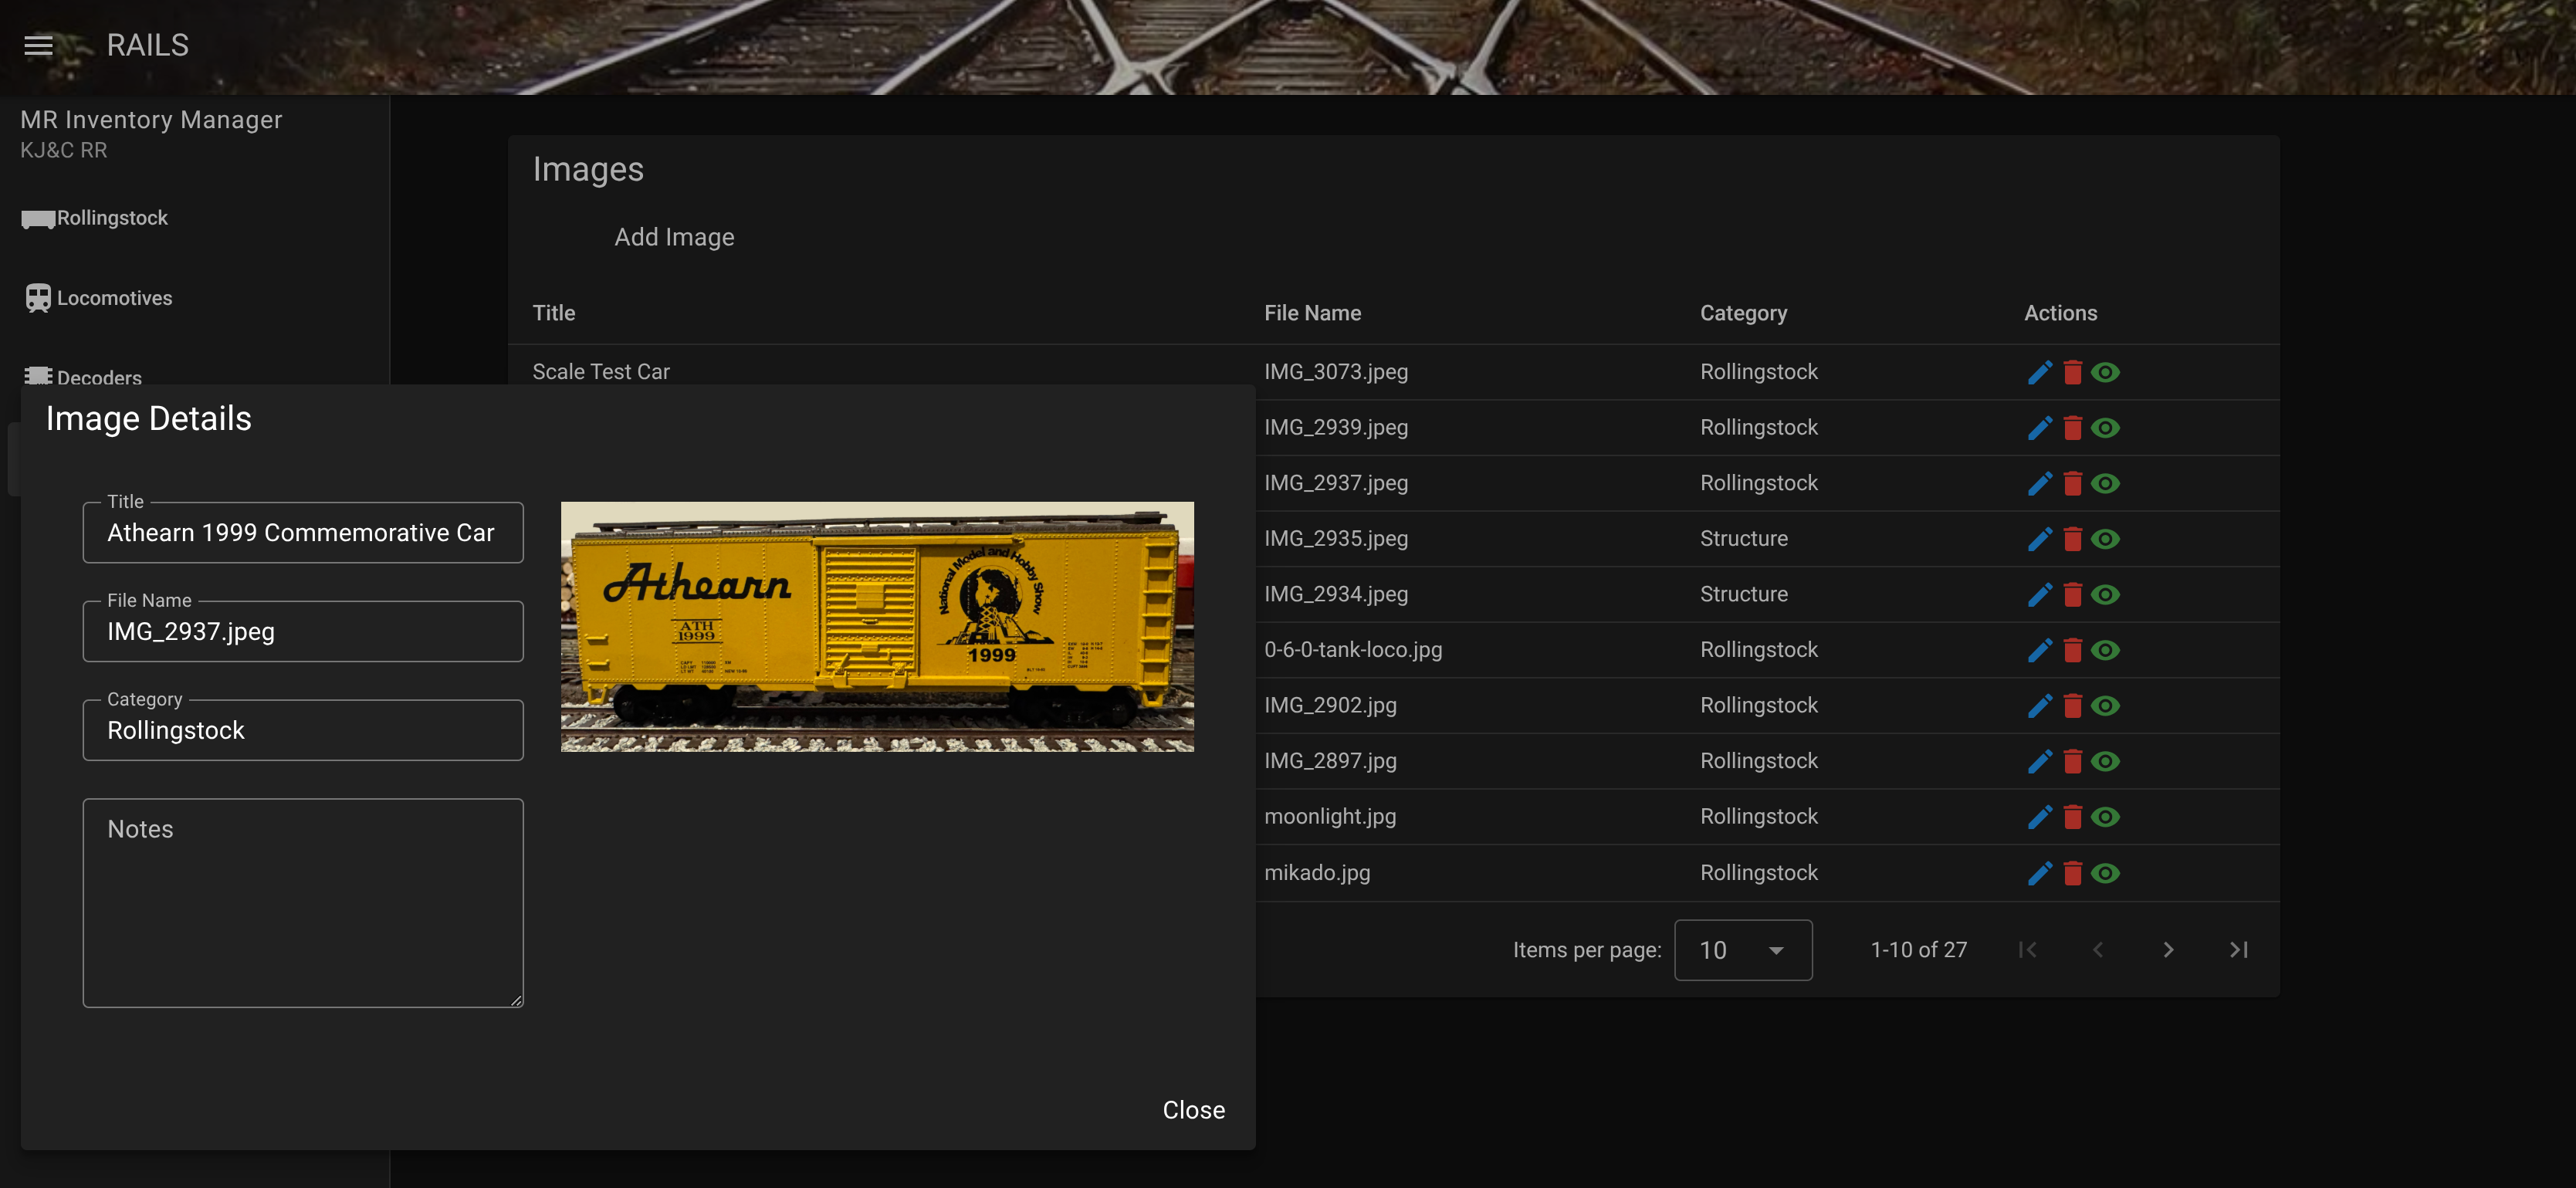
\includegraphics[width=0.85\textwidth]{./images/images-view.png}
    \caption{View Image Details}
    \label{fig:images-view}
\end{figure}

\subsection{Adding a New Image}

Clicking the "Add Image" button above the table opens a modal form for registering and uploading new graphic filesimages. The form prompts for a Title, a local File input path, a Category assignment, and optional Notes. Figure \ref{fig:images-new} illustrates the upload modal.

\begin{figure}[H]
    \centering
    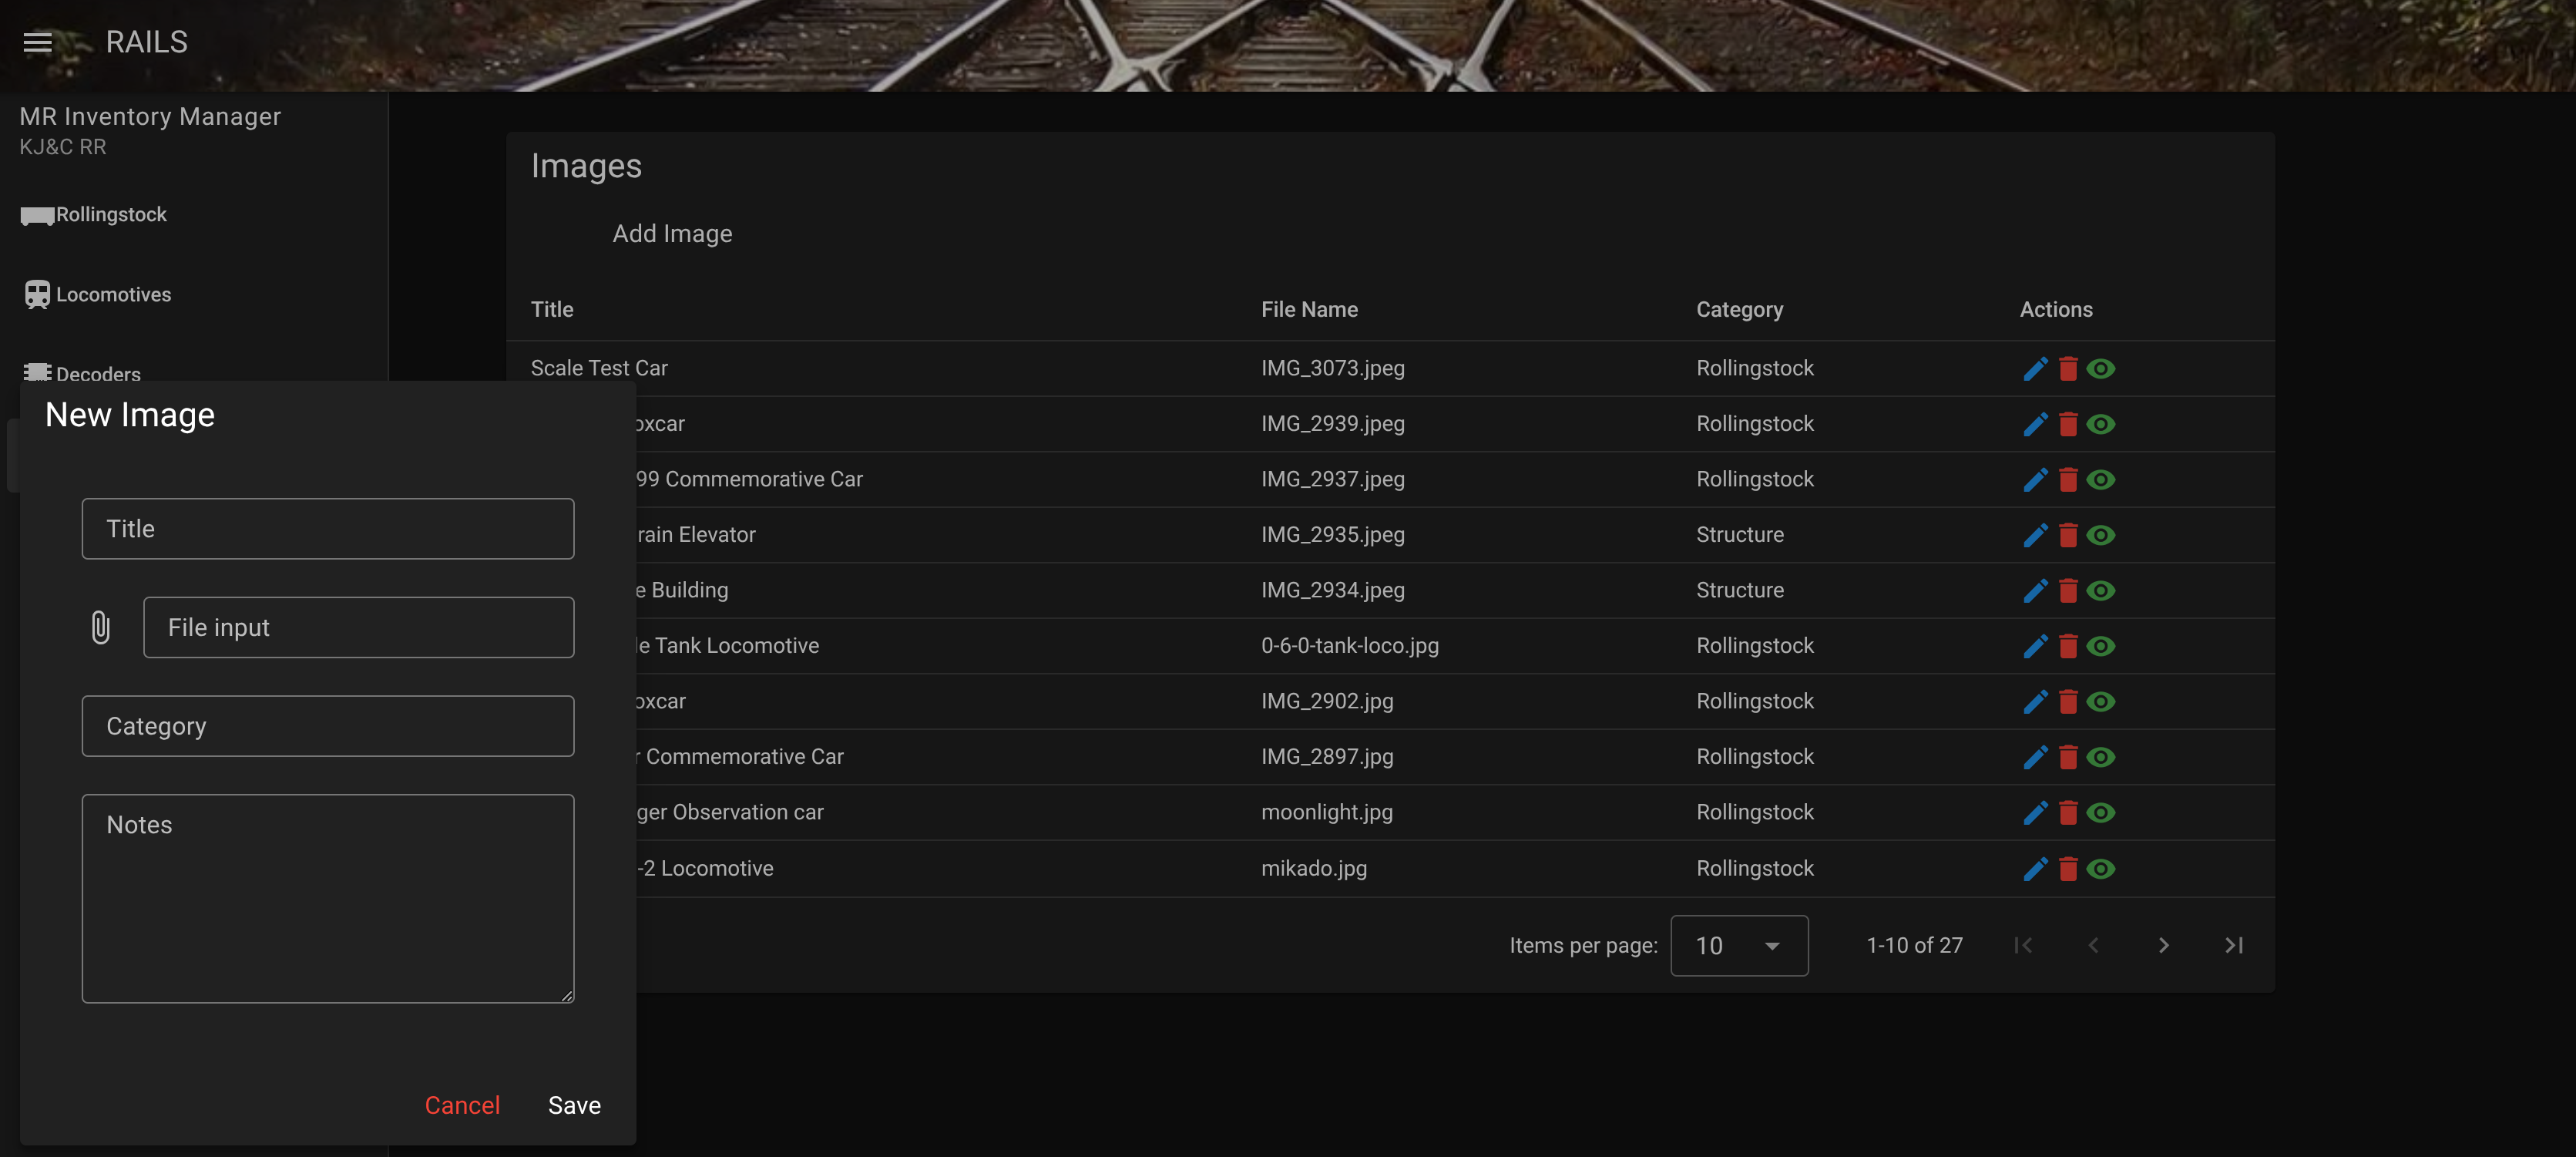
\includegraphics[width=0.85\textwidth]{./images/images-new.png}
    \caption{Add Image Dialog}
    \label{fig:images-new}
\end{figure}

\subsection{Editing Image Metadata}

To modify an existing image entry's descriptive metadata, click the blue pencil icon in the Actions columnimages. This opens the image dialog pre-populated with current values, allowing edits to the Title, File Name, Category, and Notes. Figure \ref{fig:images-edit} shows the edit dialog.

\begin{figure}[H]
    \centering
    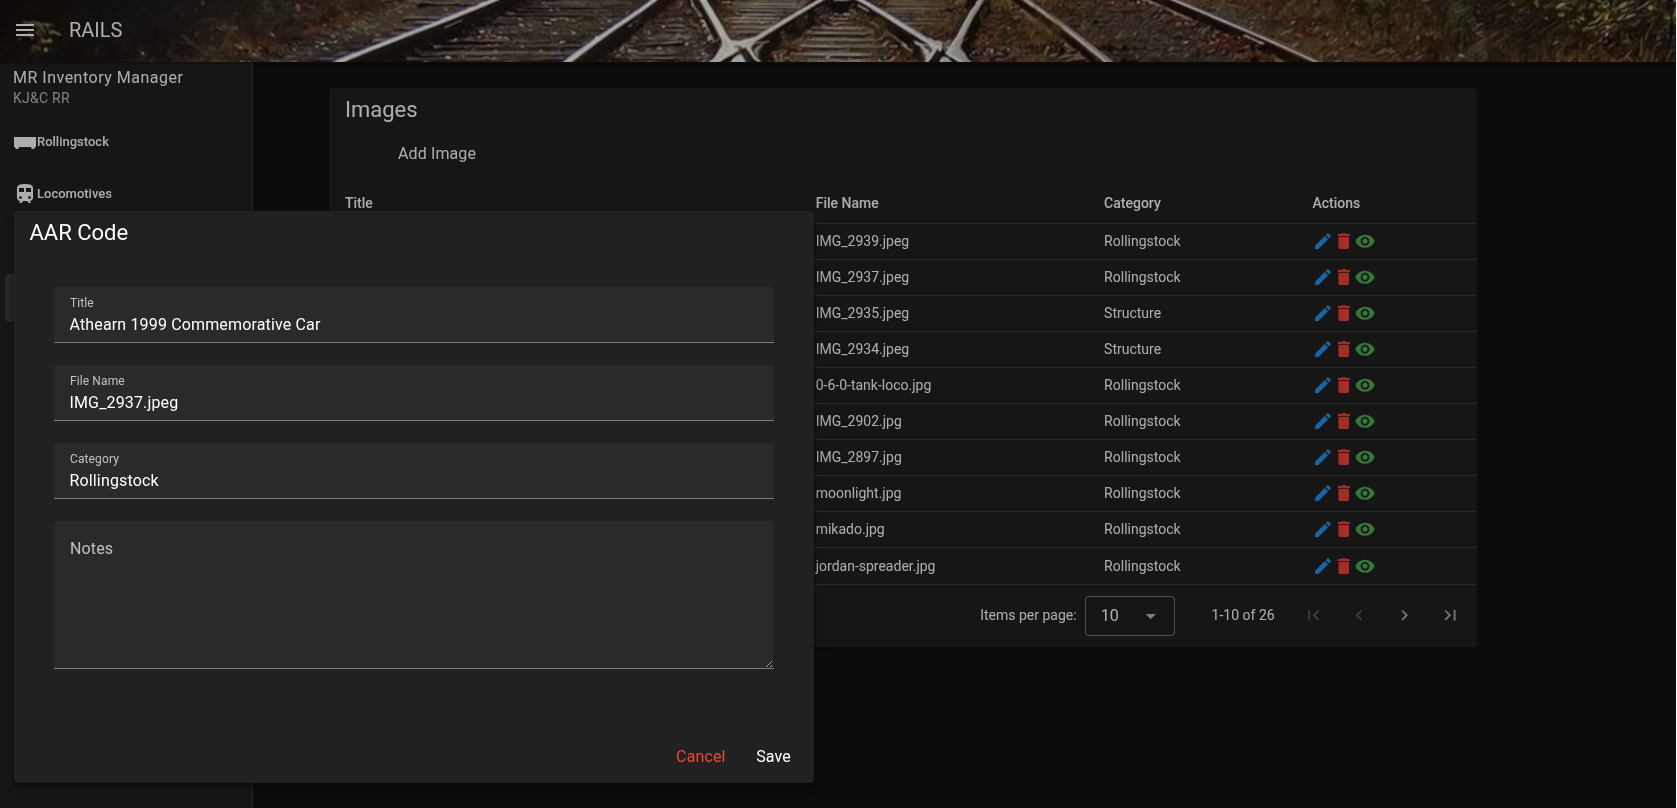
\includegraphics[width=0.85\textwidth]{./images/images-edit.png}
    \caption{Edit Image Metadata}
    \label{fig:images-edit}
\end{figure}

\subsection{Deleting Image Records}

To remove an image from the database repository, click the red trash bin icon under the Actions columnimages. A modal confirmation prompt appears requesting verification before the image asset record is deleted. Figure \ref{fig:images-delete} displays the deletion confirmation prompt.

\begin{figure}[H]
    \centering
    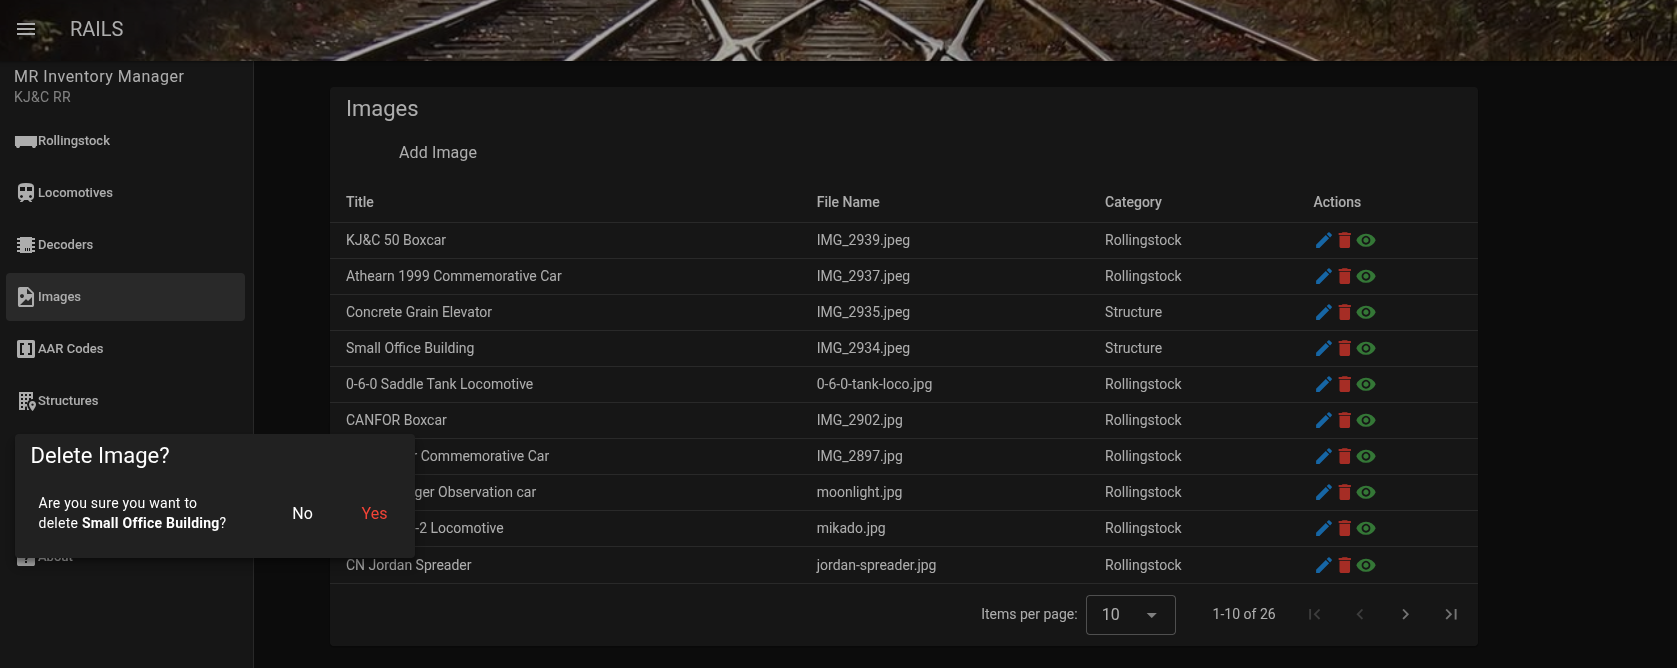
\includegraphics[width=0.85\textwidth]{./images/images-delete.png}
    \caption{Delete Image Confirmation}
    \label{fig:images-delete}
\end{figure}

\section{AAR Code Reference}

Selecting "AAR Codes" from the navigation drawer opens the Association of American Railroads (AAR) designation reference view. This page provides a standardized lookup table for rolling stock classification codes used throughout the inventory system, displaying the AAR Code, Rollingstock Type (RS Type), standard Description, and Action controls. Figure \ref{fig:aar} illustrates the main AAR Codes reference table.

\begin{figure}[H]
    \centering
    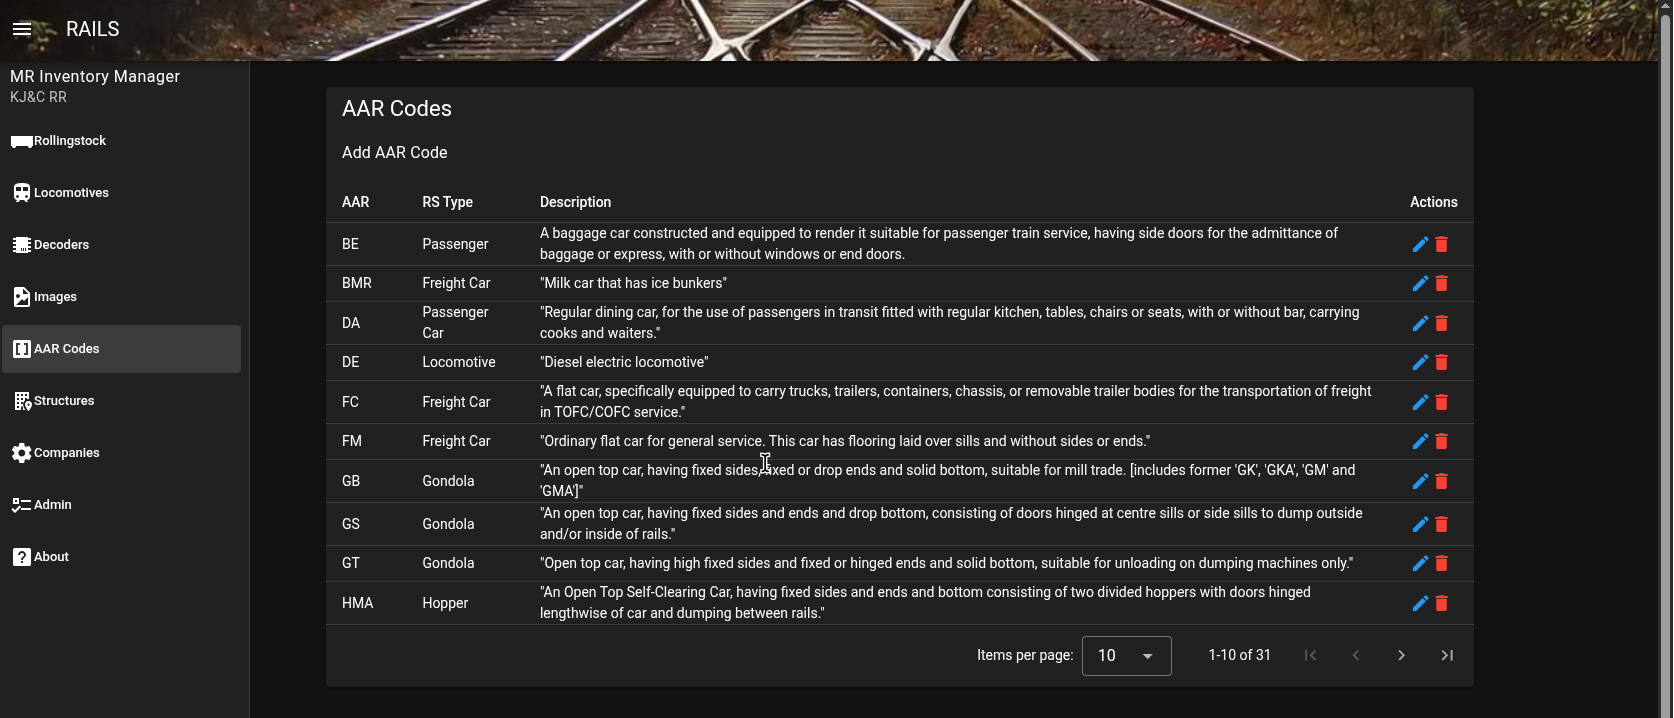
\includegraphics[width=0.85\textwidth]{./images/aar.png}
    \caption{AAR Codes Page}
    \label{fig:aar}
\end{figure}

\subsection{Adding an AAR Code}

Clicking the "Add AAR Code" button above the table opens a modal dialog to define a new equipment classification code. The form requires an AAR Code abbreviation, the associated RS Type, and a comprehensive Description detailing prototype car characteristics. Figure \ref{fig:aar-new} shows the entry modal.

\begin{figure}[H]
    \centering
    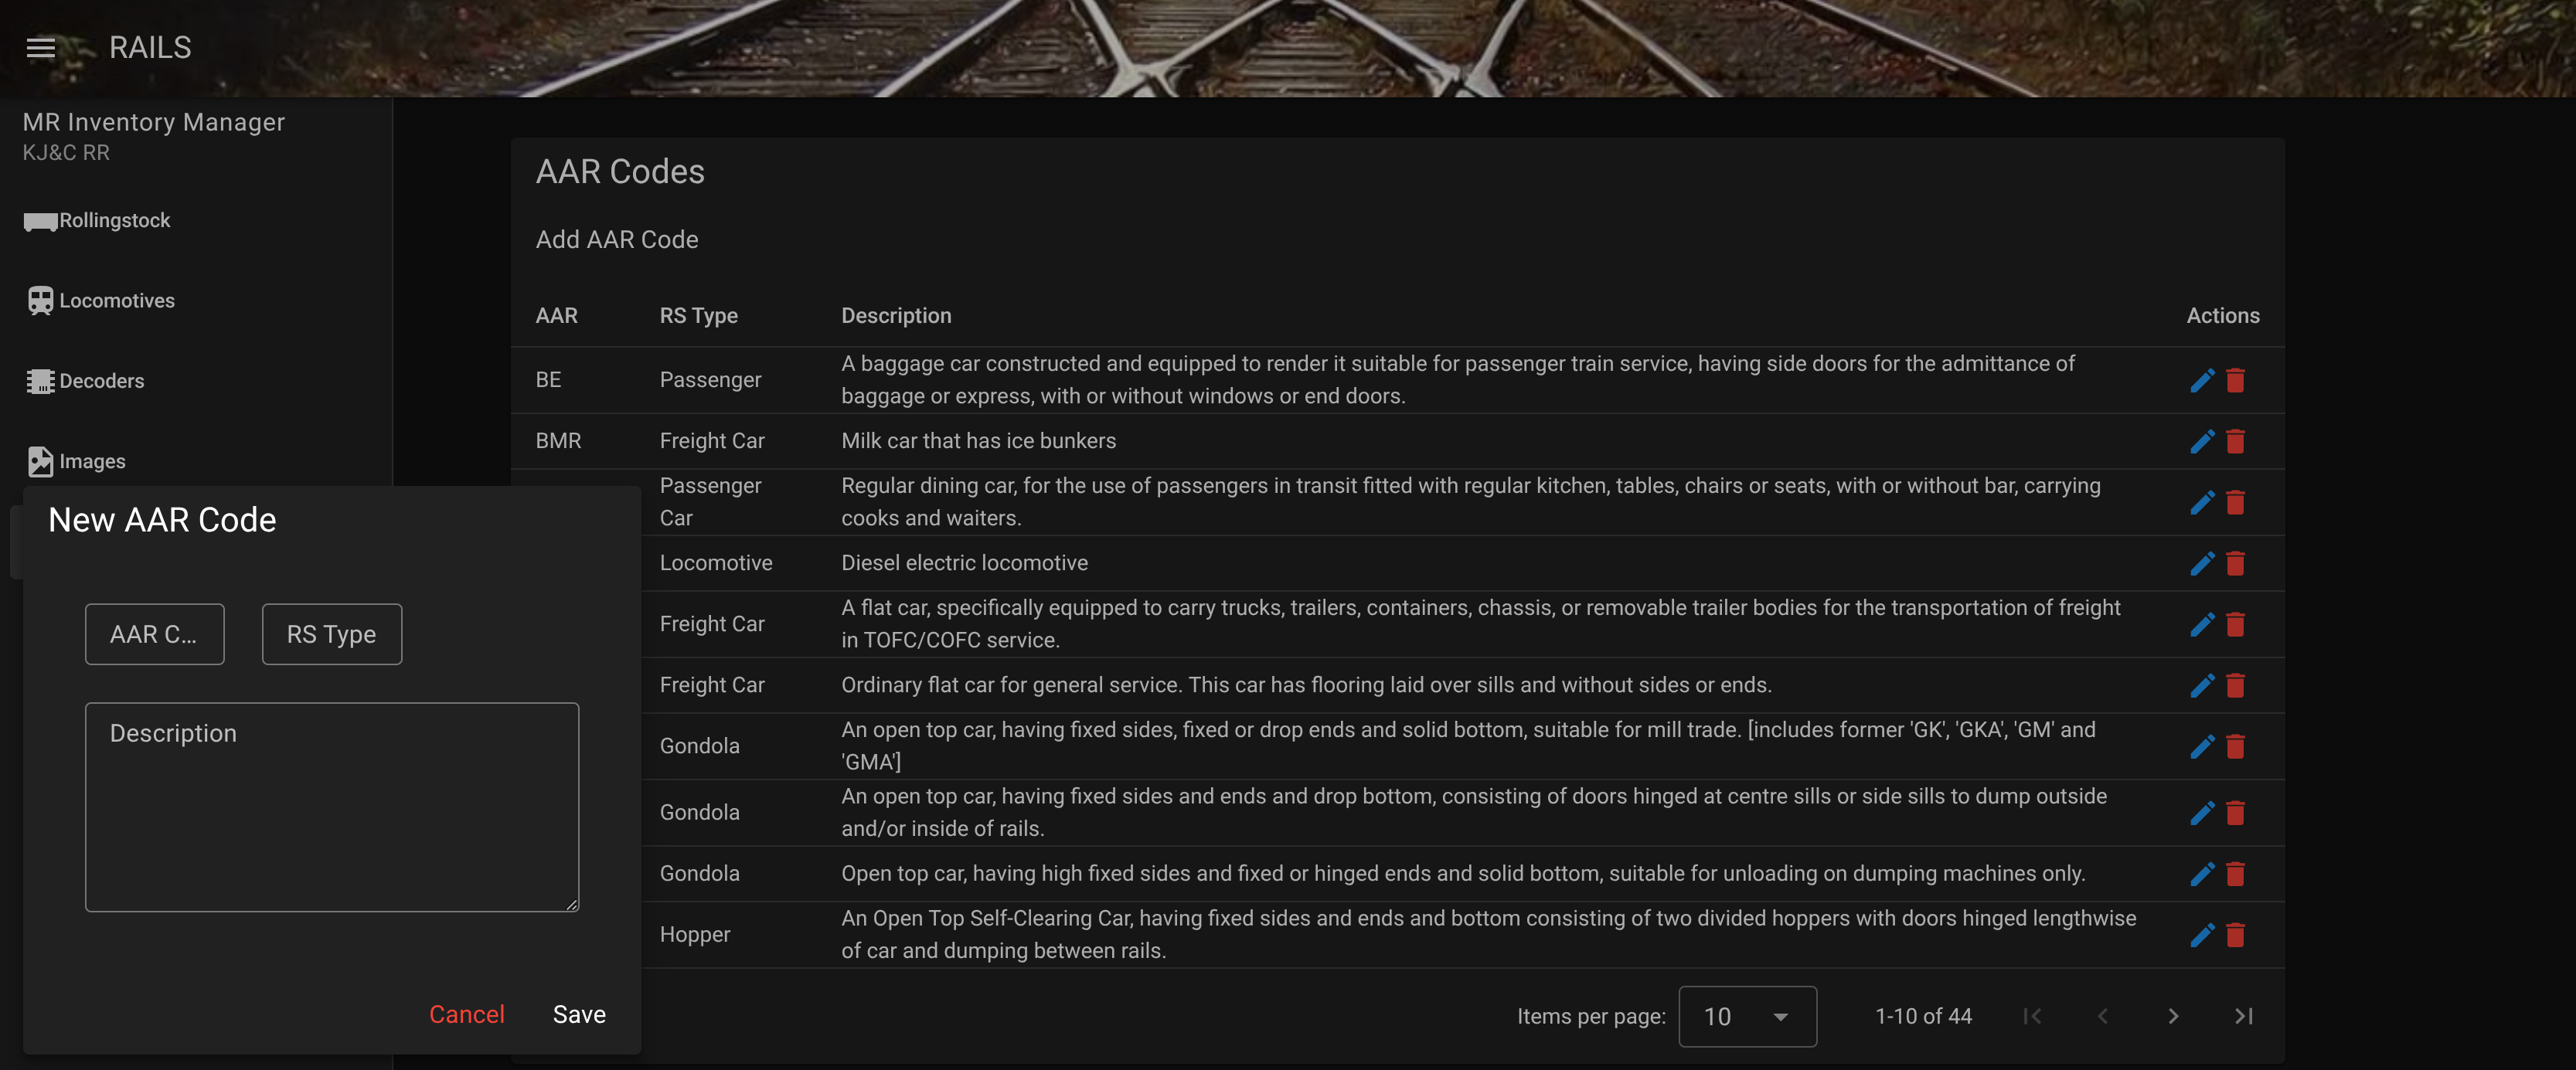
\includegraphics[width=0.85\textwidth]{./images/aar-new.png}
    \caption{Add AAR Code Dialog}
    \label{fig:aar-new}
\end{figure}

\subsection{Editing AAR Codes}

To modify an existing classification entry or update its prototype definition, click the blue pencil icon under the Actions column. This displays the AAR Code form with populated values for editing. Figure \ref{fig:aar-edit} shows the edit dialog interface.

\begin{figure}[H]
    \centering
    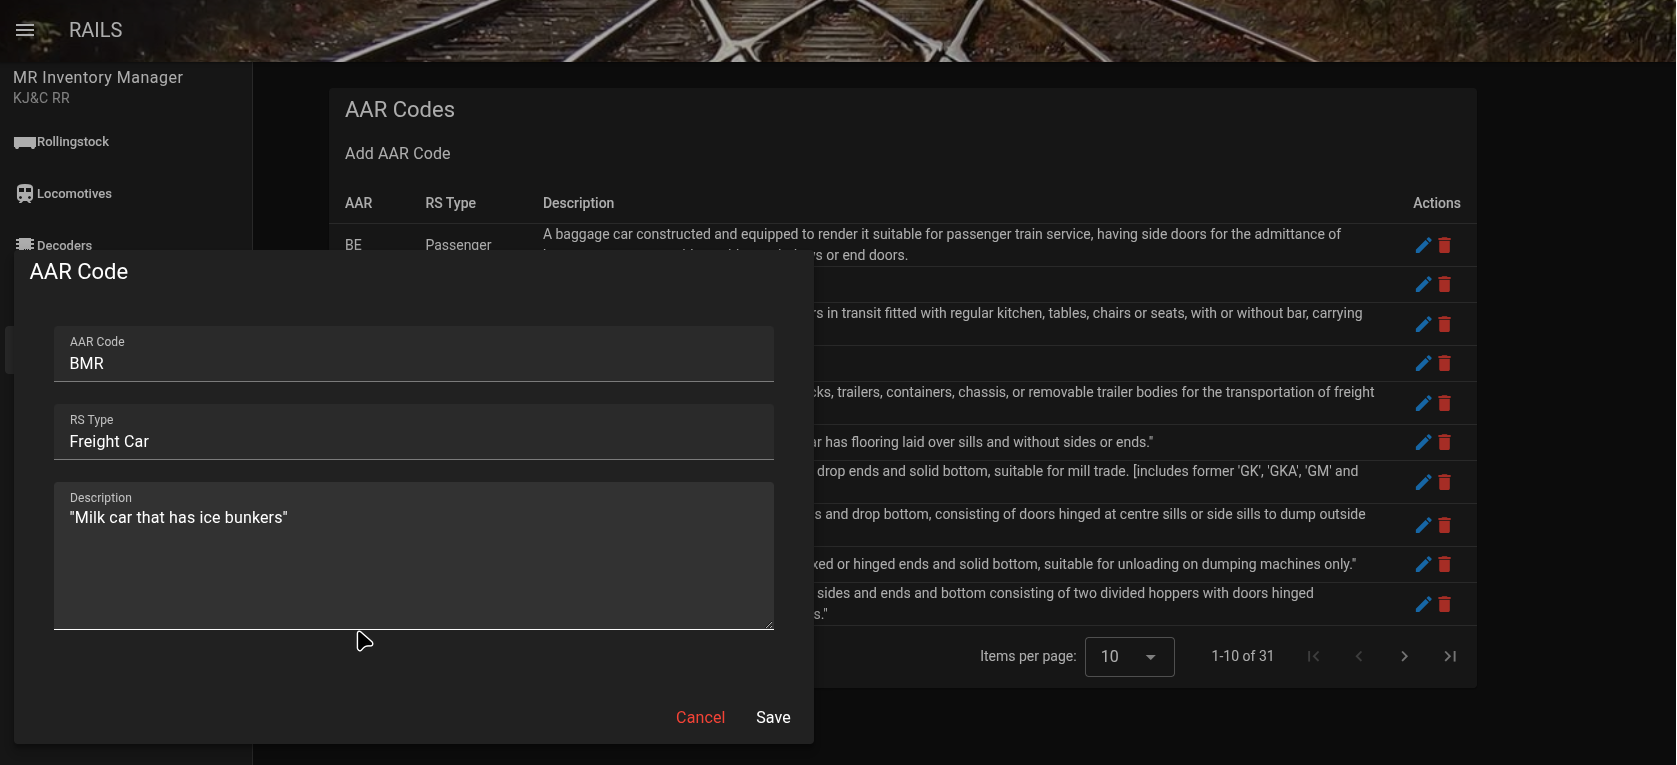
\includegraphics[width=0.85\textwidth]{./images/aar-edit.png}
    \caption{Edit AAR Code}
    \label{fig:aar-edit}
\end{figure}

\subsection{Deleting AAR Codes}

To remove a classification code from the system lookup table, click the red trash bin icon in the Actions column. A confirmation modal prompt appears requiring verification before the AAR code entry is permanently deleted. Figure \ref{fig:aar-delete} shows the deletion confirmation prompt.

\begin{figure}[H]
    \centering
    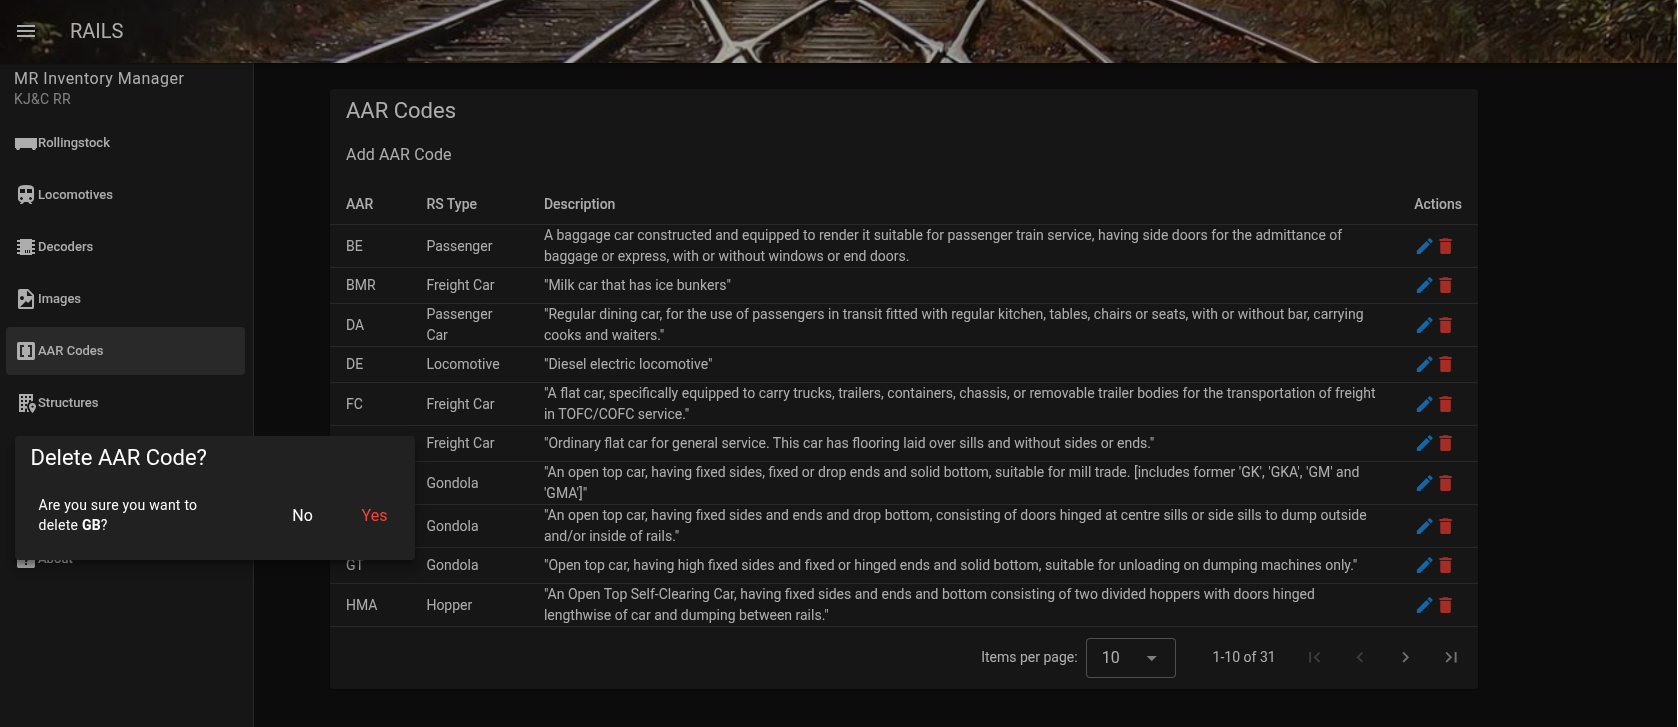
\includegraphics[width=0.85\textwidth]{./images/aar-delete.png}
    \caption{Delete AAR Code Confirmation}
    \label{fig:aar-delete}
\end{figure}

\section{Structures Management}

Selecting "Structures" from the navigation drawer displays the Structures management view. This page presents a tabular inventory of layout buildings and trackside structures, summarizing attributes such as Title, Use, Owner, layout Location, Year Built, and Action controls. Figure \ref{fig:structures} shows the main Structures table page.

\begin{figure}[H]
    \centering
    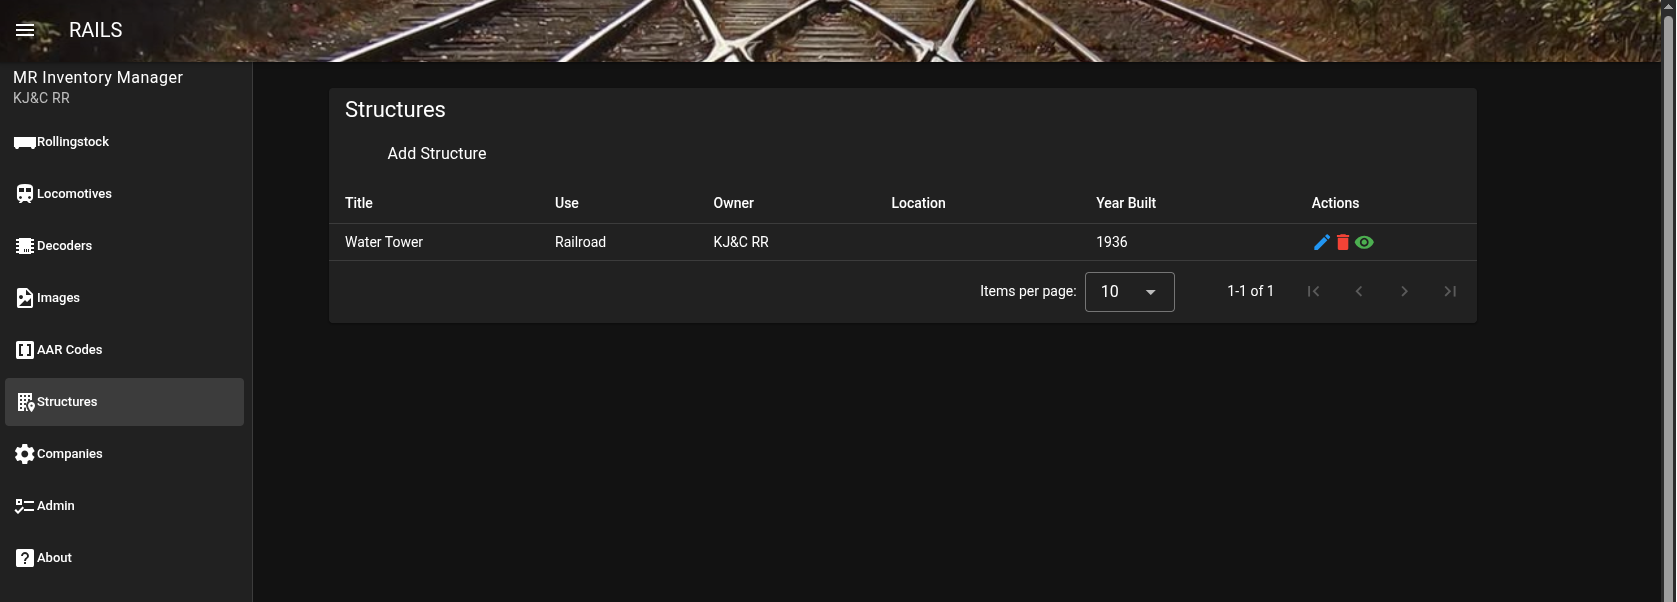
\includegraphics[width=0.85\textwidth]{./images/structures.png}
    \caption{Structures Page}
    \label{fig:structures}
\end{figure}

\subsection{Viewing Structure Details}

Clicking the green eye icon in the Actions column opens a detail view modal. This dialog presents recorded attributes alongside an embedded photo preview of the modeled structure. Figure \ref{fig:structures-view} displays the structure inspection dialog.

\begin{figure}[H]
    \centering
    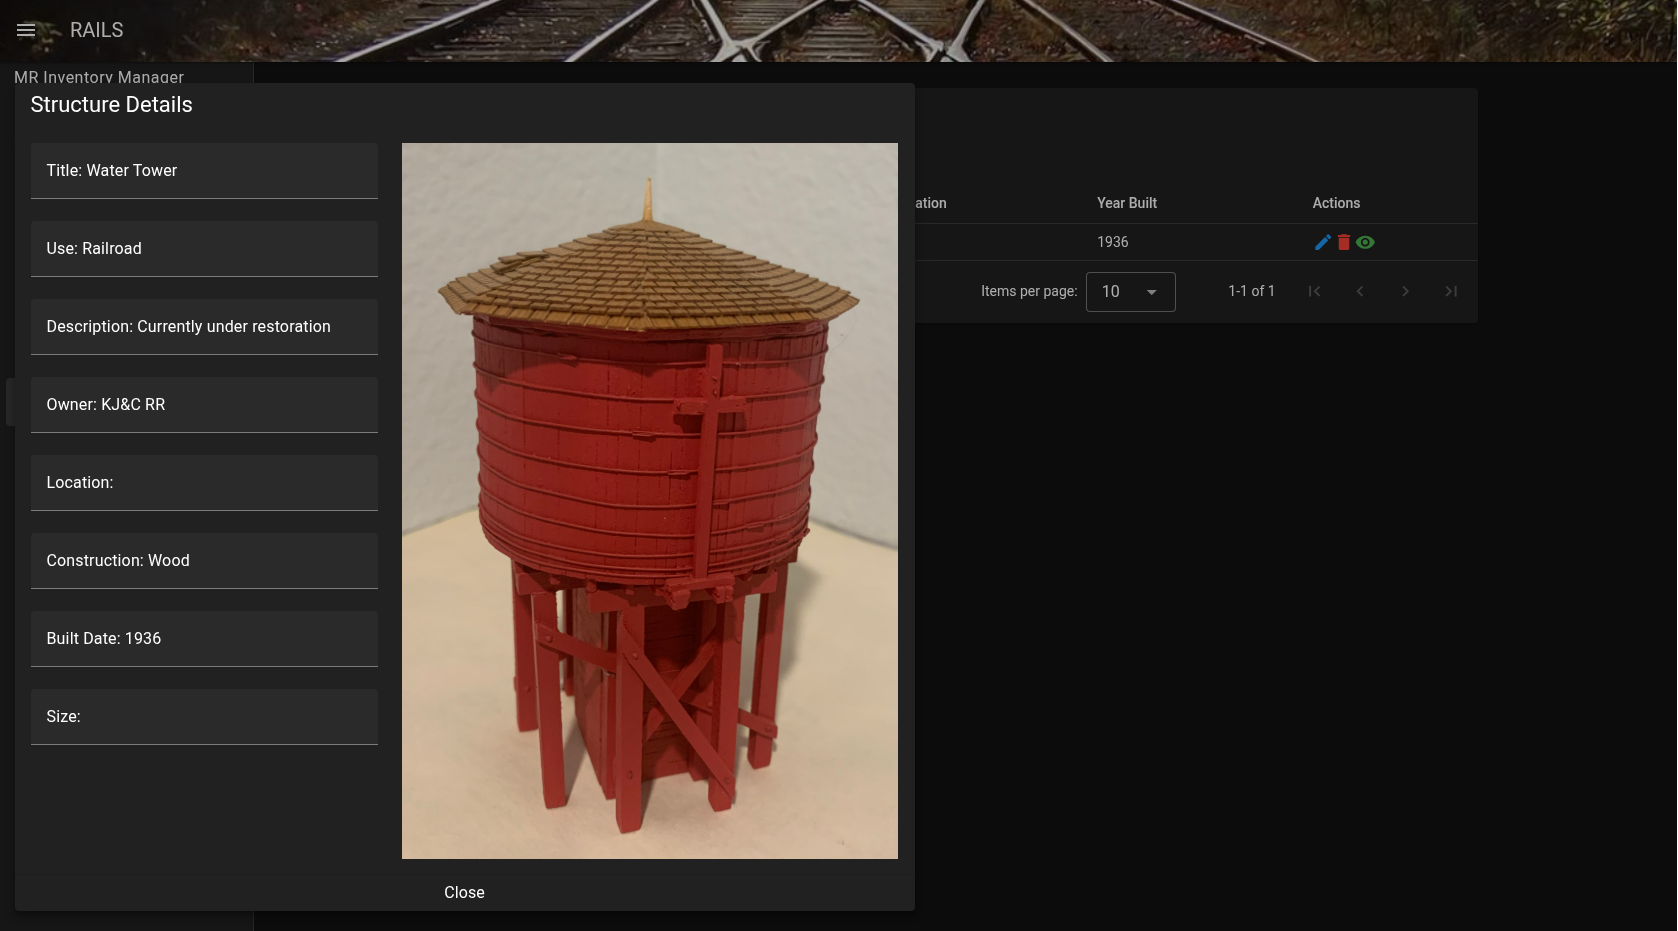
\includegraphics[width=0.85\textwidth]{./images/structures-view.png}
    \caption{View Structure Details}
    \label{fig:structures-view}
\end{figure}

\subsection{Adding a New Structure}

Clicking the "Add Structure" button above the table opens a modal dialog for adding a new building or facility to the database. The form includes comprehensive fields for general metadata (Title, Use, Owner, Location, Construction, Built Date, Size, Image) and operational parameters (Industrial classification, Type, Raw Materials, Capacities, Production Rates, Priority, AAR Codes In/Out, Load/Unload Durations, Siding Capacity, and Notes). Figure \ref{fig:structures-new} illustrates the structure creation modal.

\begin{figure}[H]
    \centering
    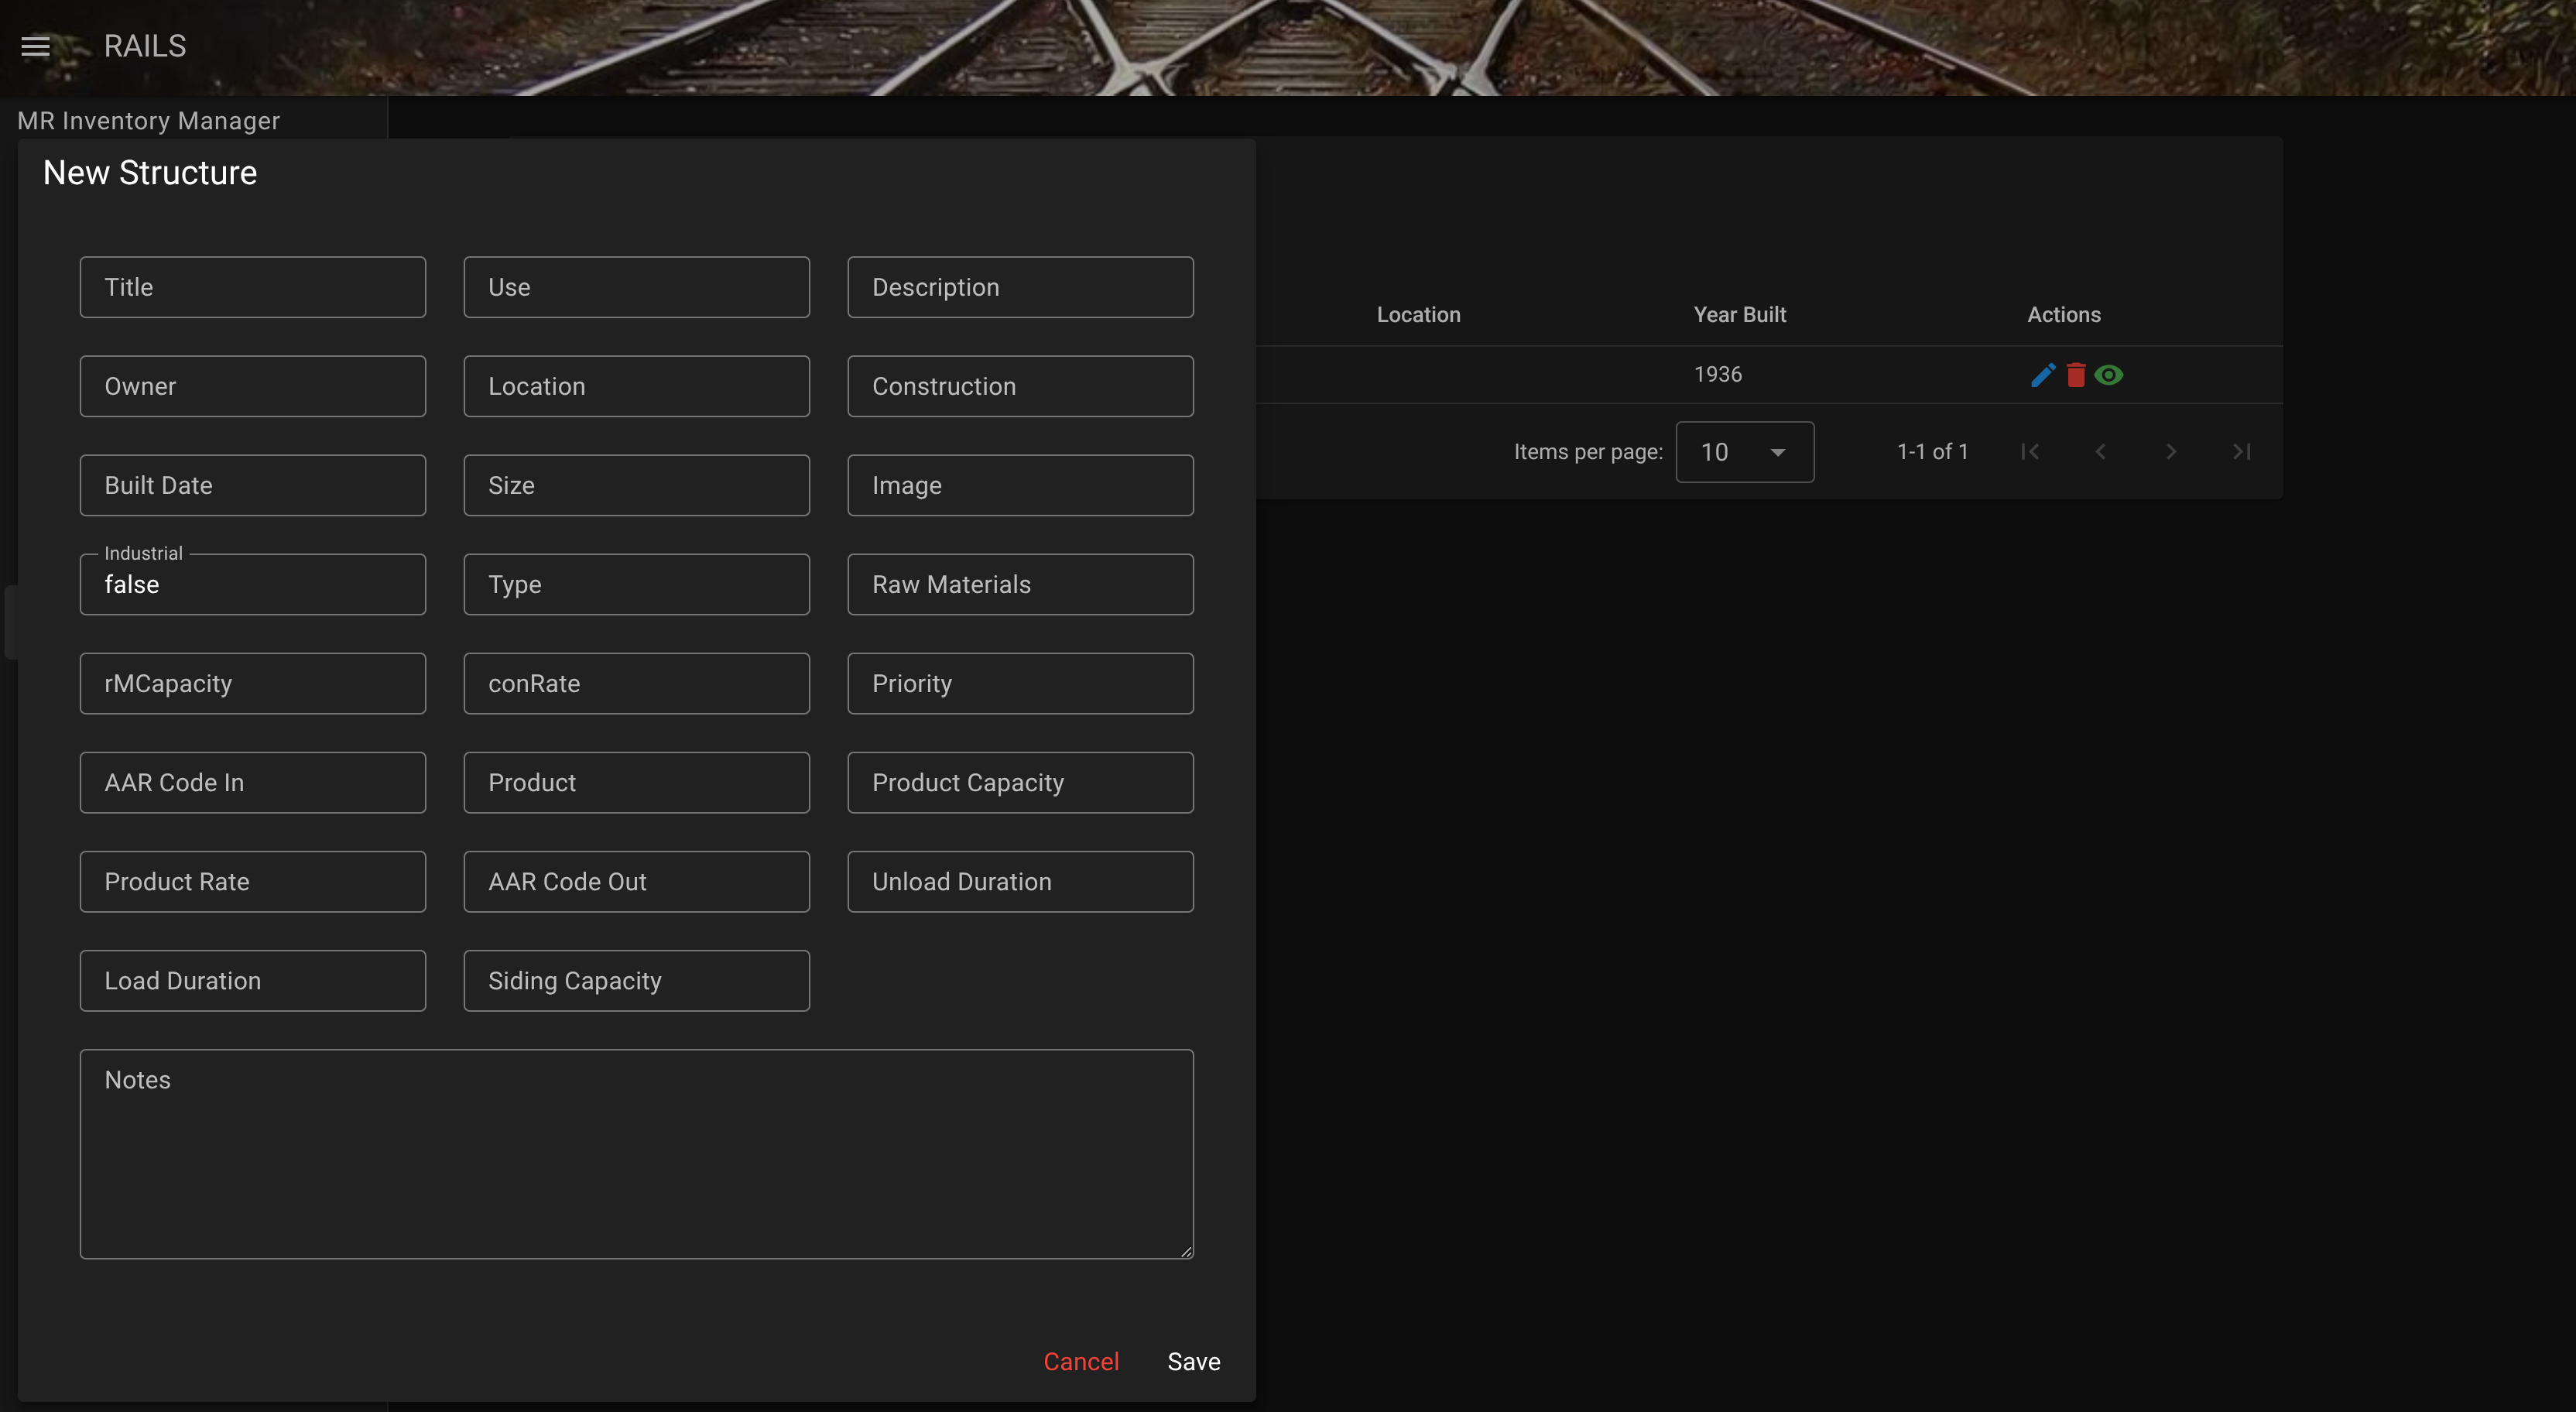
\includegraphics[width=0.85\textwidth]{./images/structures-new.png}
    \caption{Add Structure Dialog}
    \label{fig:structures-new}
\end{figure}

\subsection{Editing Structure Records}

To update an existing entry, click the blue pencil icon under the Actions column. This opens the structure form populated with current records, allowing edits to physical attributes, image references, or industrial operational data. Figure \ref{fig:structures-edit} shows the edit structure dialog.

\begin{figure}[H]
    \centering
    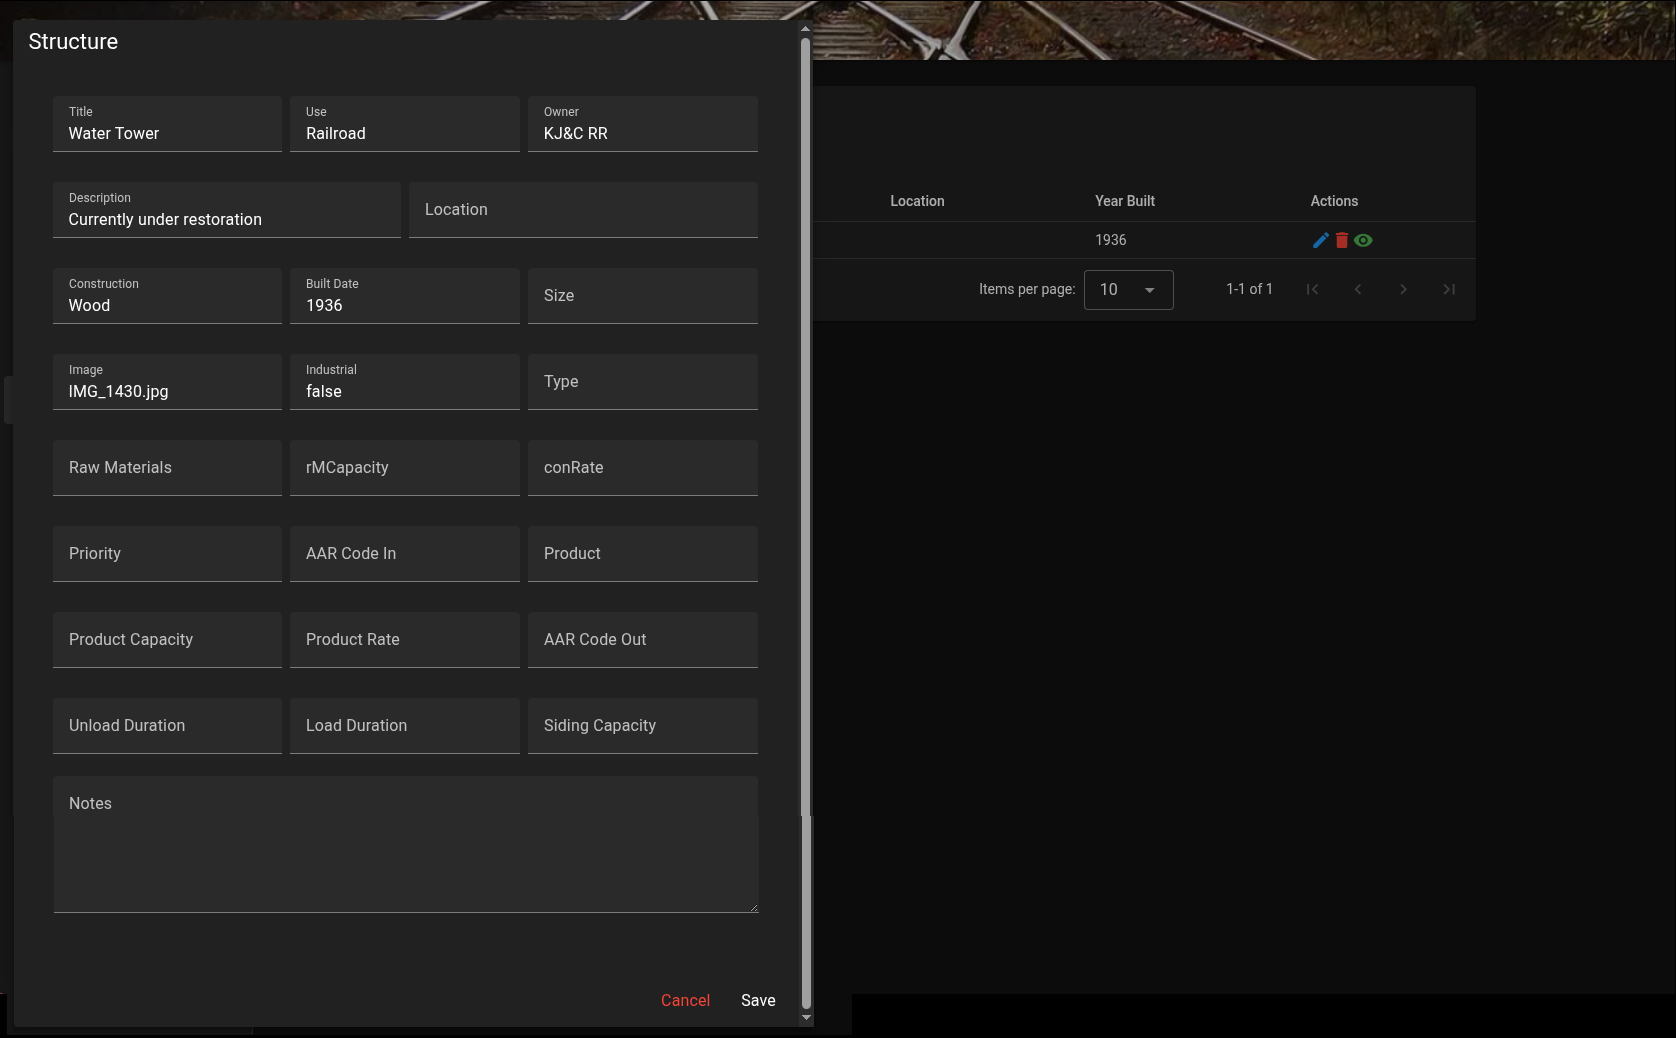
\includegraphics[width=0.85\textwidth]{./images/structures-edit.png}
    \caption{Edit Structure}
    \label{fig:structures-edit}
\end{figure}

\subsection{Deleting Structure Records}

To remove a structure entry from the inventory, click the red trash bin icon in the Actions column. A confirmation prompt appears requiring verification before the record is deleted from the system database. Figure \ref{fig:structures-delete} illustrates the deletion modal dialog.

\begin{figure}[H]
    \centering
    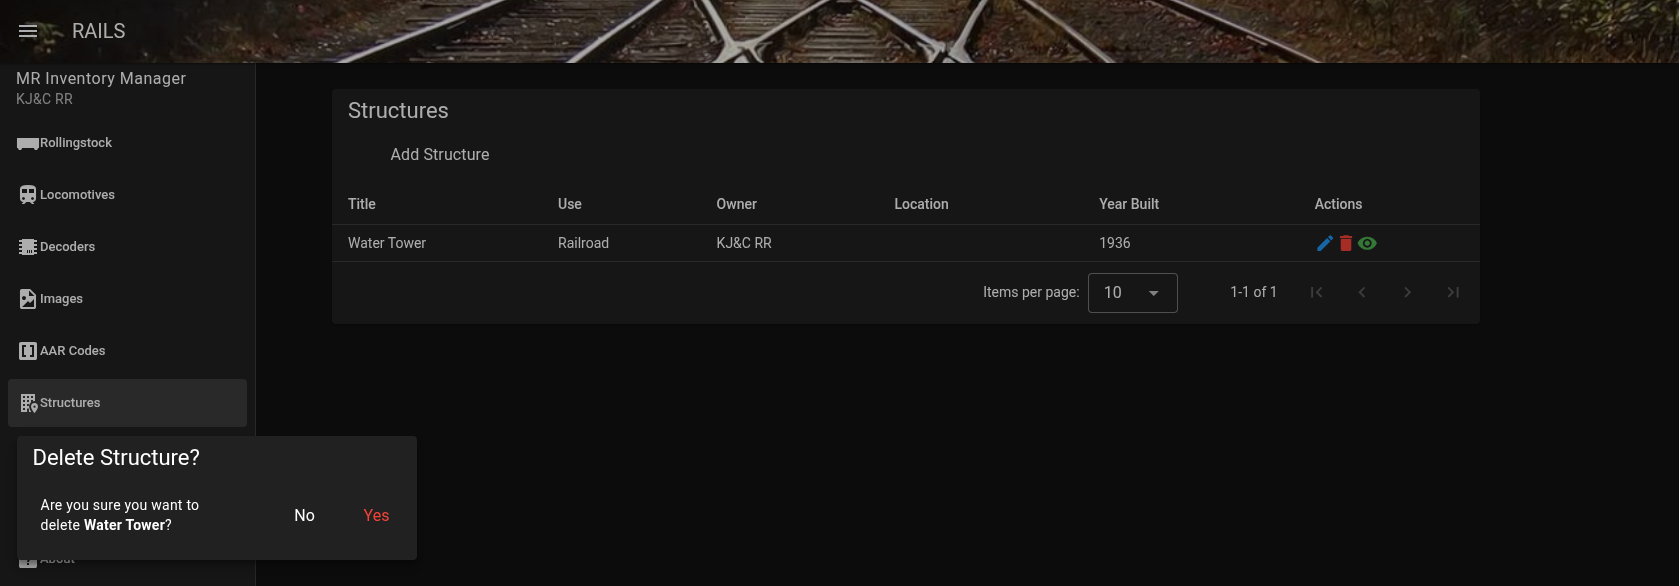
\includegraphics[width=0.85\textwidth]{./images/structures-delete.png}
    \caption{Delete Structure Confirmation}
    \label{fig:structures-delete}
\end{figure}

\section{Companies Reference}

Selecting "Companies" from the navigation drawer opens the Companies management view. This page serves as a central reference table for railroad equipment manufacturers, locomotive builders, and operating railway companies. It displays the company short Name (abbreviation), Full Name, Type classification (e.g., Builder, Railway), Location, and Action controls. Figure \ref{fig:companies} illustrates the main Companies page interface.

\begin{figure}[H]
    \centering
    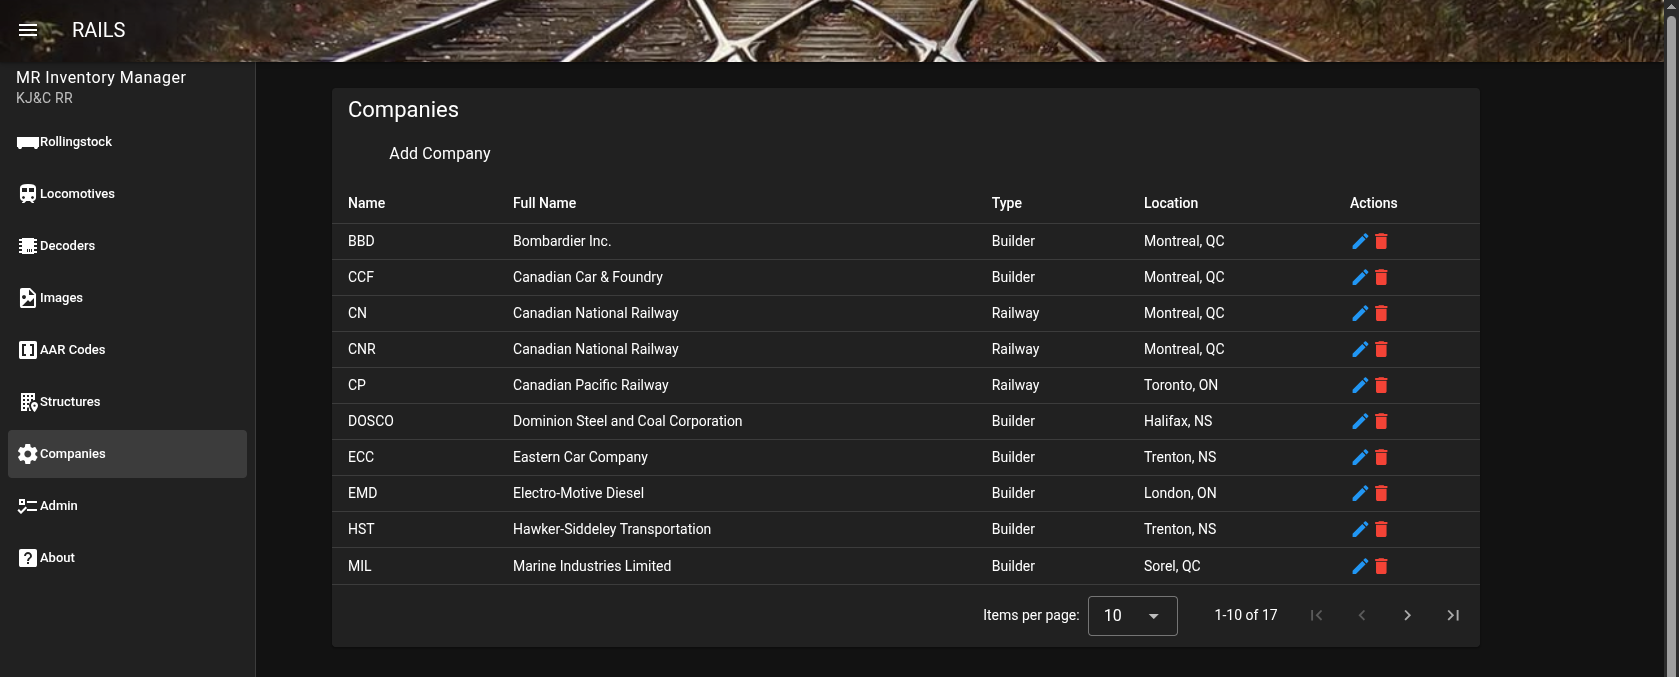
\includegraphics[width=0.85\textwidth]{./images/companies.png}
    \caption{Companies Page}
    \label{fig:companies}
\end{figure}

\subsection{Adding a Company}

Clicking the "Add Company" button above the table opens a modal dialog to define a new corporate entry. The form prompts for the company's short Name, Long Name, Type (such as Builder or Railway), and headquarters Location. Figure \ref{fig:companies-new} shows the company entry modal.

\begin{figure}[H]
    \centering
    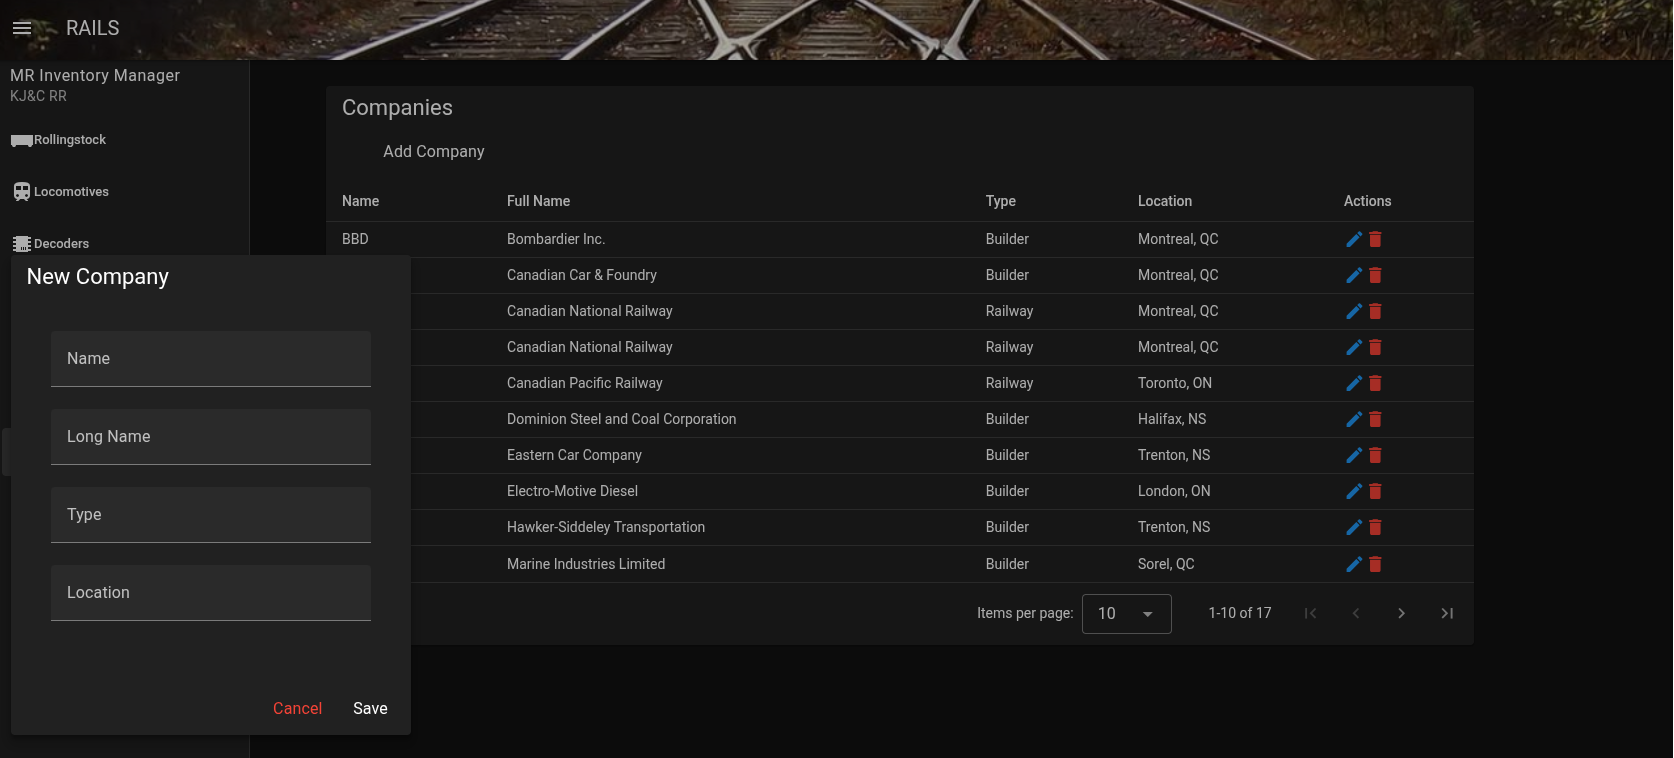
\includegraphics[width=0.85\textwidth]{./images/companies-new.png}
    \caption{Add Company Dialog}
    \label{fig:companies-new}
\end{figure}

\subsection{Editing Company Records}

To modify an existing company entry, click the blue pencil icon under the Actions column. This opens the edit dialog populated with current information, allowing adjustments to reporting marks, full corporate titles, or location details. Figure \ref{fig:companies-edit} displays the edit company interface.

\begin{figure}[H]
    \centering
    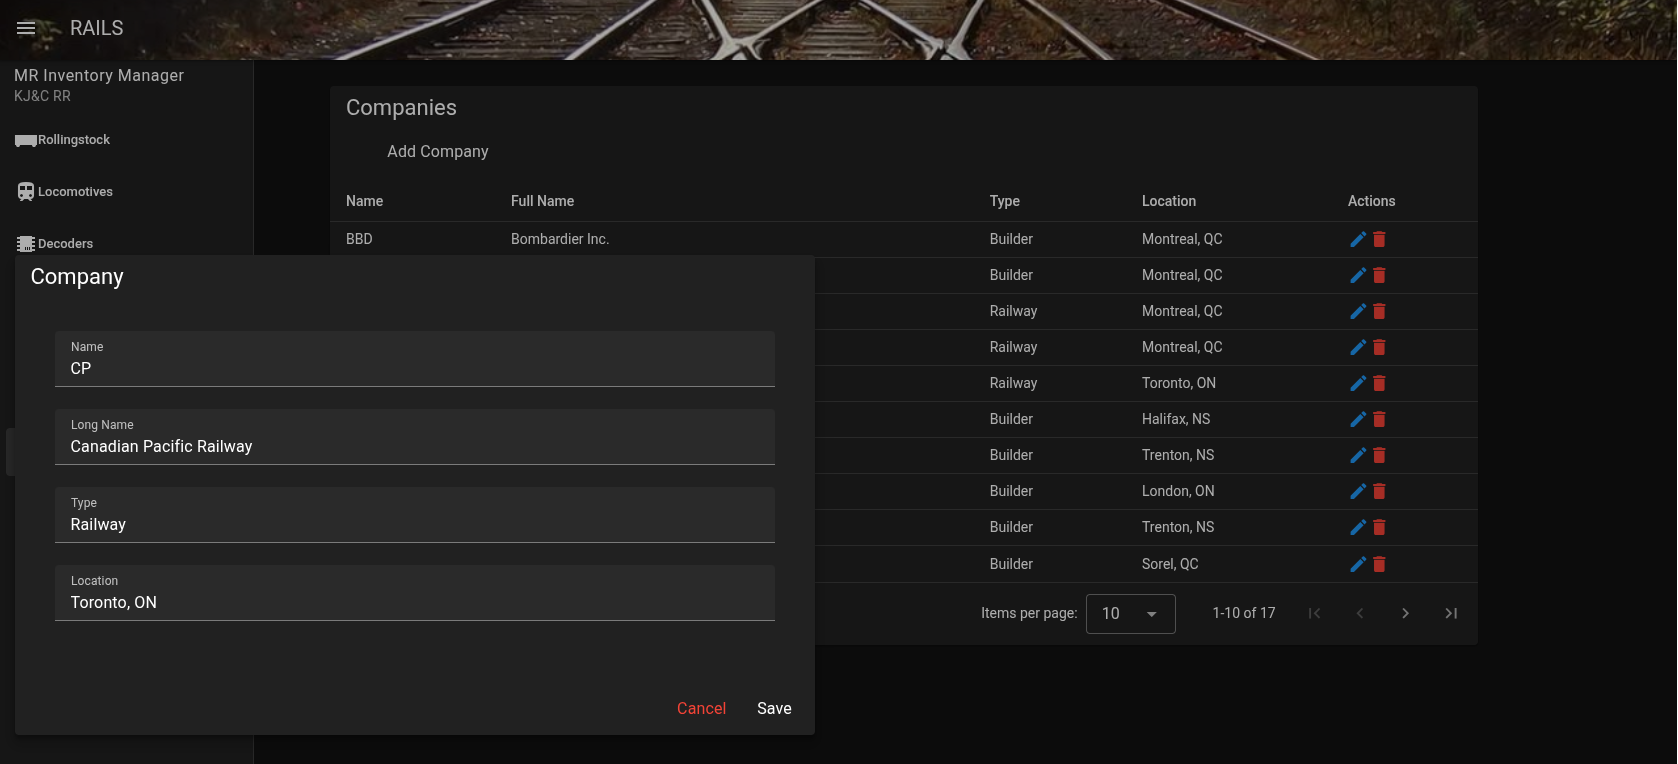
\includegraphics[width=0.85\textwidth]{./images/companies-edit.png}
    \caption{Edit Company}
    \label{fig:companies-edit}
\end{figure}

\subsection{Deleting Company Records}

To remove a corporate entity from the system reference table, click the red trash bin icon in the Actions column. A confirmation prompt appears asking for verification before removing the company entry. Figure \ref{fig:companies-delete} shows the deletion confirmation prompt dialog.

\begin{figure}[H]
    \centering
    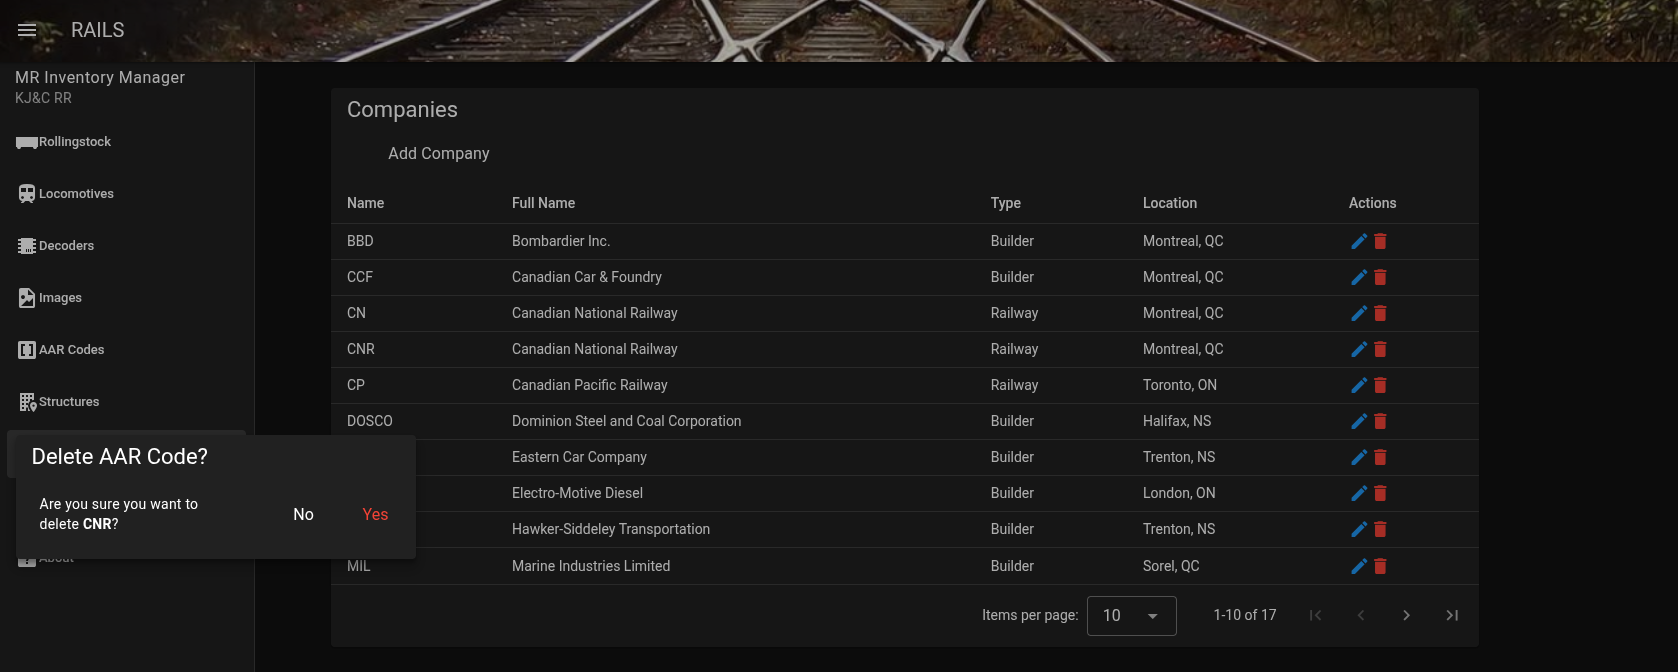
\includegraphics[width=0.85\textwidth]{./images/companies-delete.png}
    \caption{Delete Company Confirmation}
    \label{fig:companies-delete}
\end{figure}

\section{Admin Dashboard}

Selecting "Admin" from the navigation drawer opens the Admin dashboard view. This page provides centralized controls for system data management, including database collection exports, imports, report generation, and car card printing. Figure \ref{fig:admin} shows the main Admin page interface.

\begin{figure}[H]
    \centering
    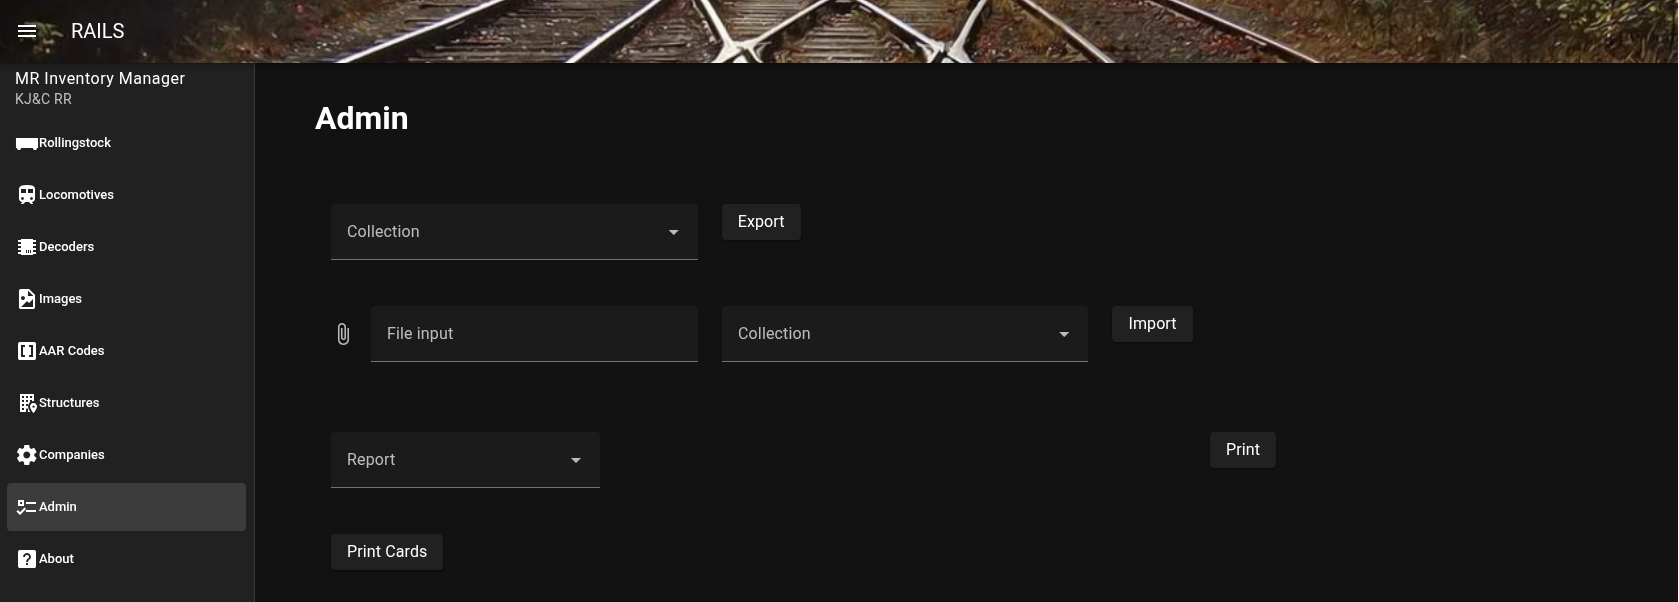
\includegraphics[width=0.85\textwidth]{./images/admin.png}
    \caption{Admin Page}
    \label{fig:admin}
\end{figure}

\subsection{Exporting Data Collections}

The Export control allows backup or data extraction of individual system collections. Selecting the "Collection" dropdown opens a list of available data sets, including AAR Codes, Companies, Images, Rolling Stock, Decoders, and Structures. Figure \ref{fig:admin-ex-collection} illustrates the collection selection menu for data export.

\begin{figure}[H]
    \centering
    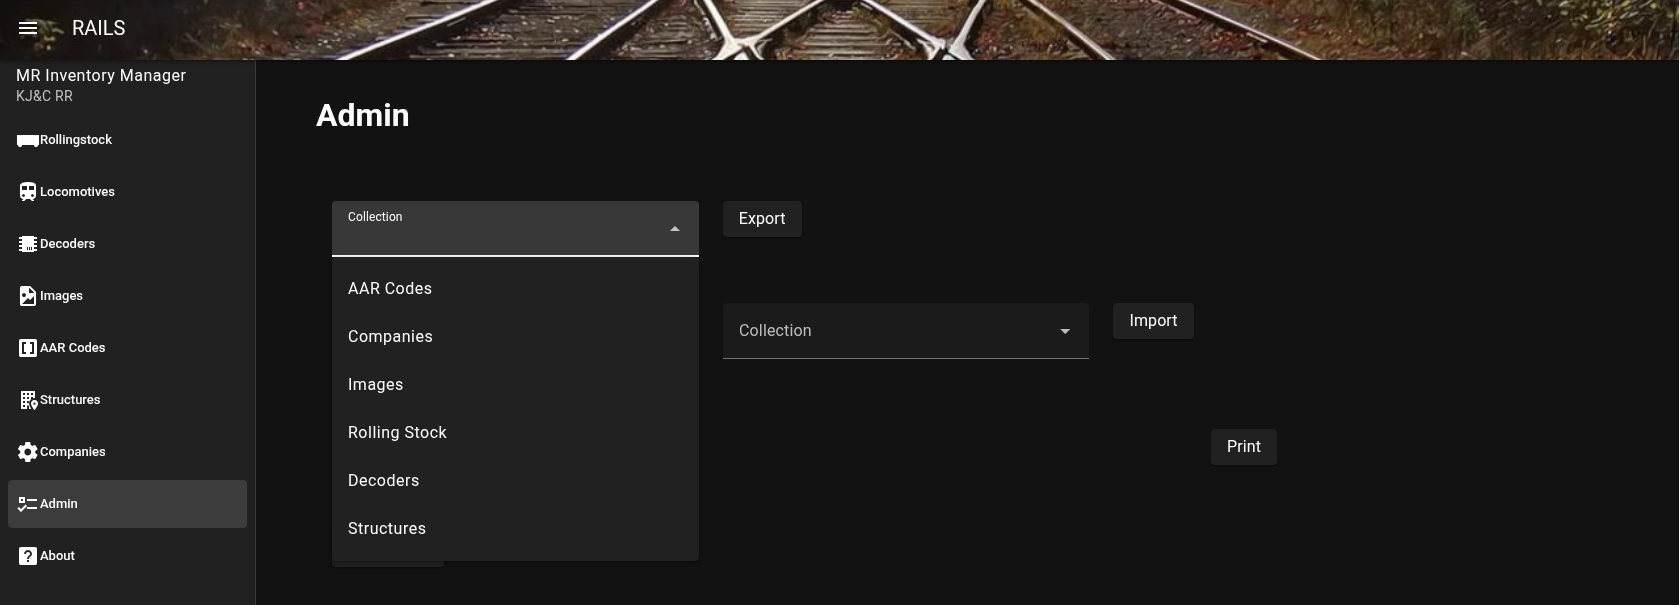
\includegraphics[width=0.85\textwidth]{./images/admin-ex-collection.png}
    \caption{Select Export Collection}
    \label{fig:admin-ex-collection}
\end{figure}

\subsection{Importing Data Collections}

To restore or bulk-load records, click the paperclip icon or file input field to launch the system file browser and select a local source file. Figure \ref{fig:admin-in-file} shows the native file chooser selection dialog.

\begin{figure}[H]
    \centering
    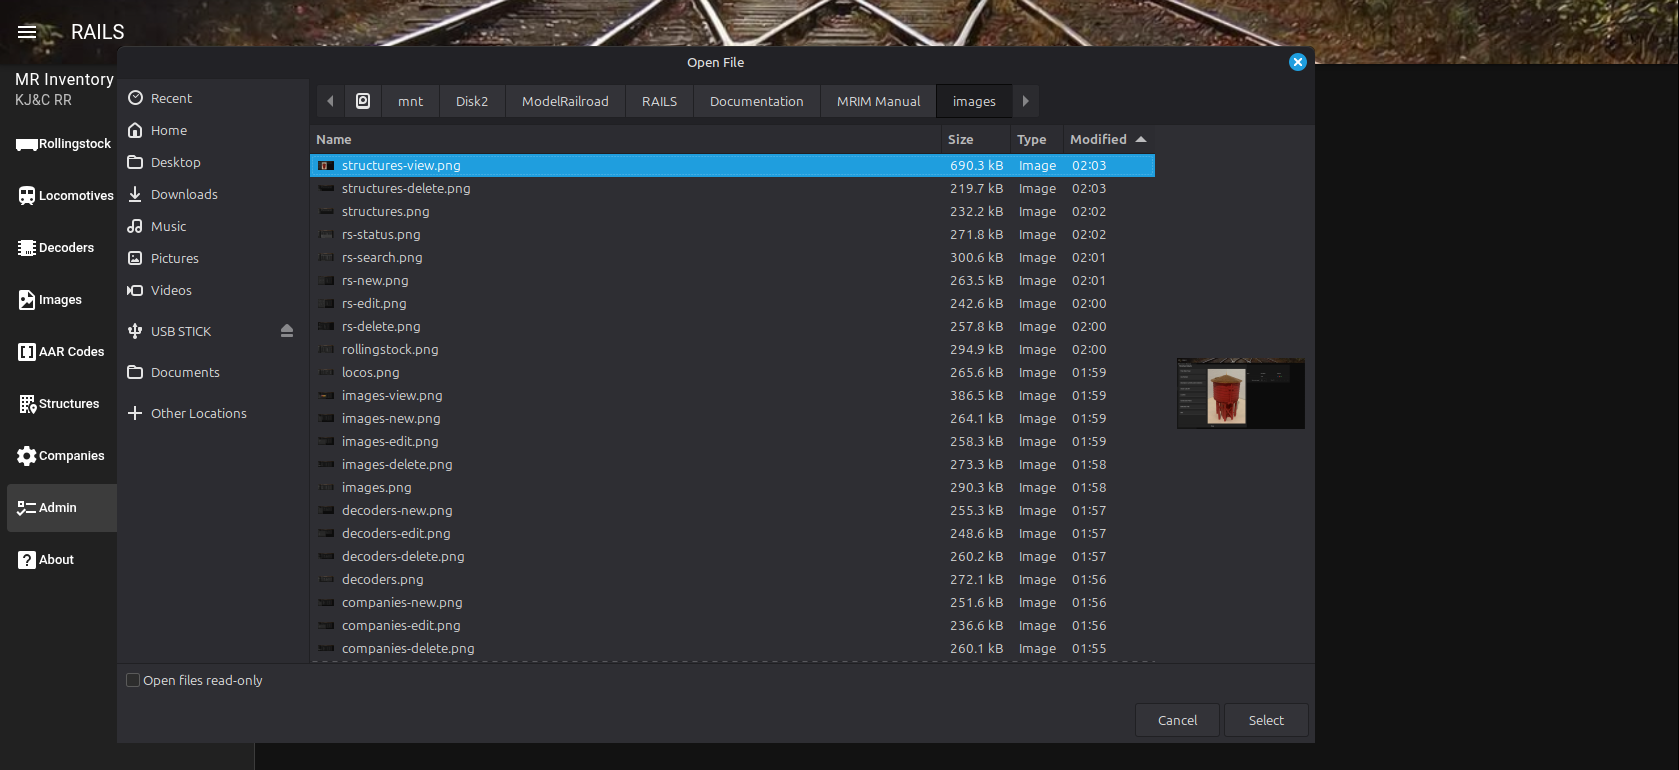
\includegraphics[width=0.85\textwidth]{./images/admin-in-file.png}
    \caption{Select Import Source File}
    \label{fig:admin-in-file}
\end{figure}

After specifying a source file, select the target database destination using the "Collection" dropdown menu. Options include AAR Codes, Companies, Images, Rolling Stock, Decoders, and Structures. Figure \ref{fig:admin-in-collection} illustrates selecting the target import collection before clicking "Import".

\begin{figure}[H]
    \centering
    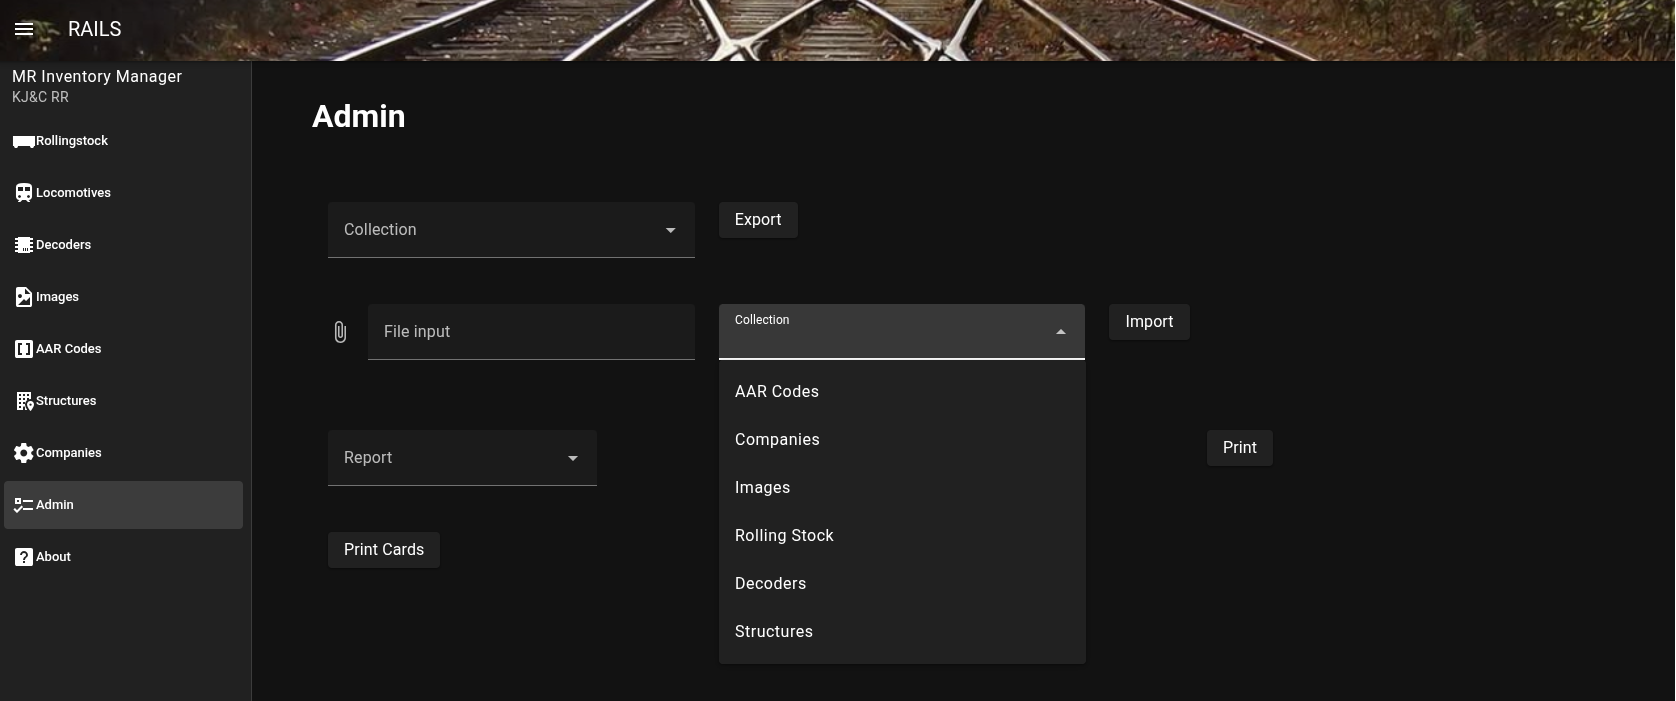
\includegraphics[width=0.85\textwidth]{./images/admin-in-collection.png}
    \caption{Select Target Import Collection}
    \label{fig:admin-in-collection}
\end{figure}

\subsection{Generating System Reports}

The Report section generates formatted system documentation and operational materials as a \gls{pdf} format. Selecting the "Report" dropdown displays available system inventories and assets for export, such as Rolling Stock, AAR Codes, Companies, Images, RFID, and Structures. Figure \ref{fig:admin-report} shows the report type selection menu.

\begin{figure}[H]
    \centering
    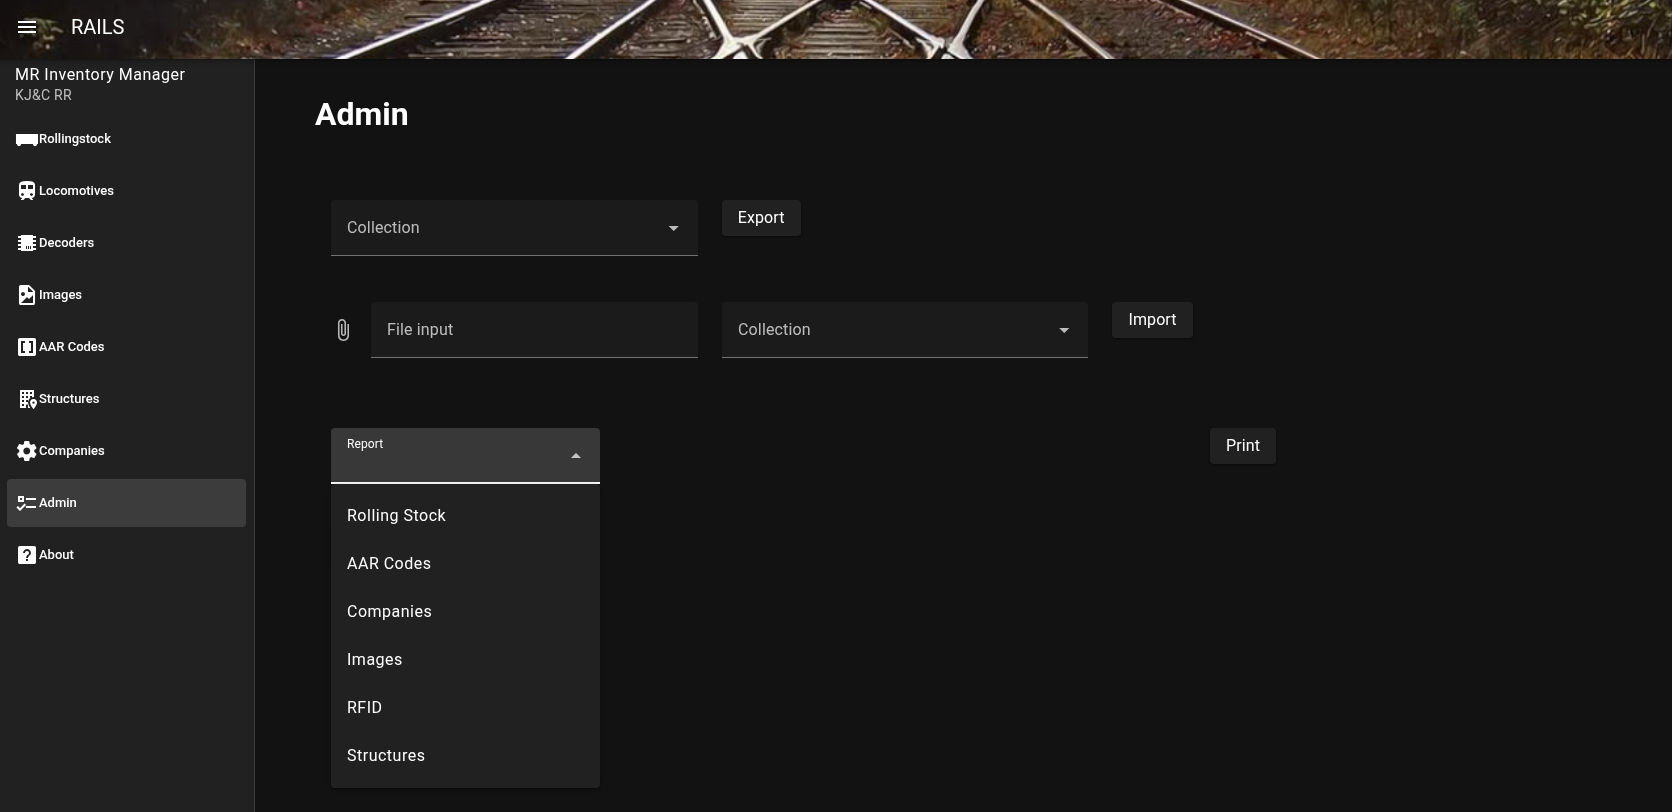
\includegraphics[width=0.85\textwidth]{./images/admin-report.png}
    \caption{Select Report Category}
    \label{fig:admin-report}
\end{figure}

When a specific report category like Rolling Stock is selected, additional sorting options appear. Clicking the "Sorted By" dropdown allows records to be ordered by parameters such as Road Names, AAR Codes, or Status. Figure \ref{fig:admin-rpt-rs-sort} illustrates the sorting criteria options.

\begin{figure}[H]
    \centering
    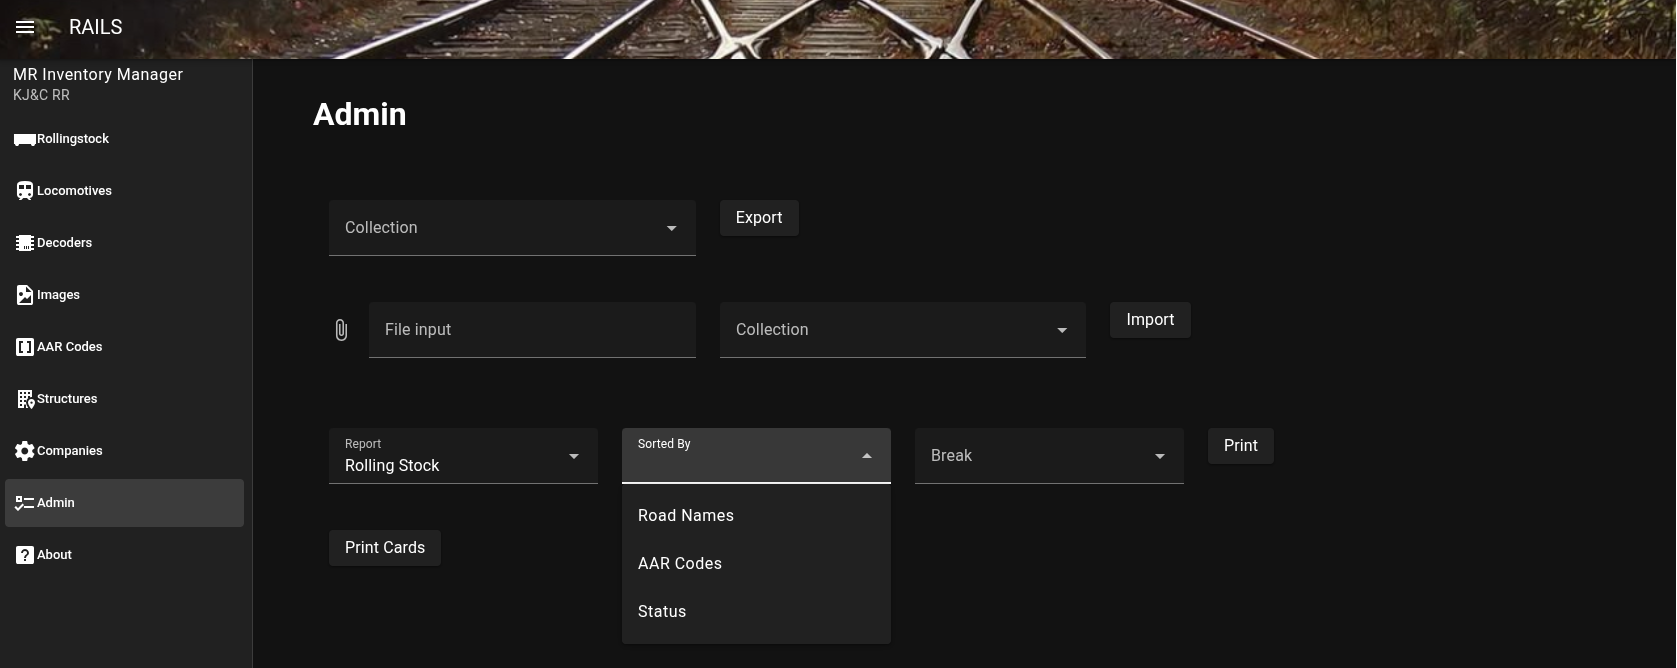
\includegraphics[width=0.85\textwidth]{./images/admin-rpt-rs-sort.png}
    \caption{Report Sort Options}
    \label{fig:admin-rpt-rs-sort}
\end{figure}

Reports can also be structured using page breaks or formatting style options. Selecting the "Break" dropdown provides options for Continuous formatting, Table views, or explicit Page breaks between sections. Figure \ref{fig:admin-rpt-rs-breaki} shows the report page break selection menu.

\begin{figure}[H]
    \centering
    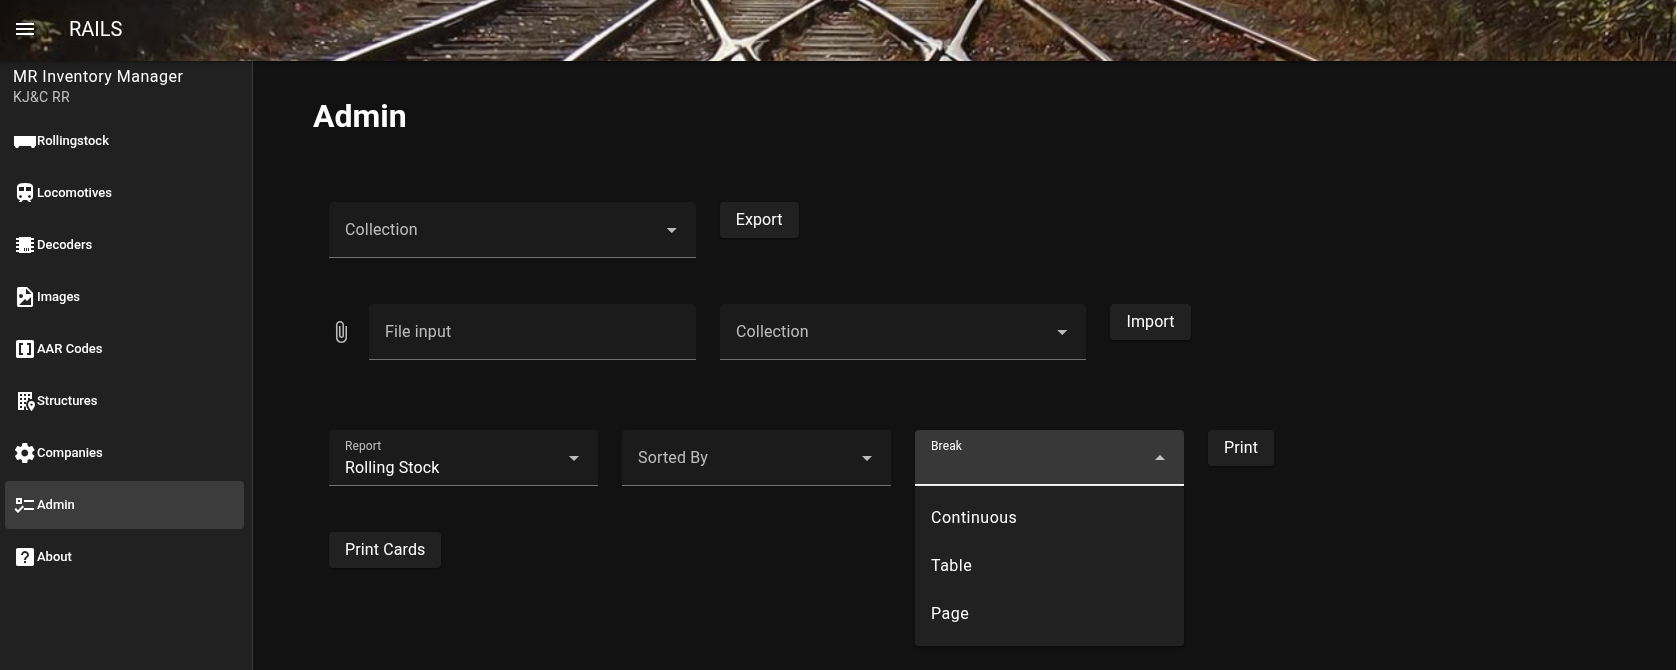
\includegraphics[width=0.85\textwidth]{./images/admin-rpt-rs-breaki.png}
    \caption{Report Page Break Formatting}
    \label{fig:admin-rpt-rs-breaki}
\end{figure}

Clicking on the "Print Cards" creates a set of pages that canbe cut into car cards used as a two-part system to track freight cars and simulate real-world cargo movements across a layout.

%%========================================================================
\backmatter

\printnoidxglossary[type=\acronymtype, sort=letter, title={Acronyms}, style=list]

\end{document}
